\documentclass[twoside]{article}
%-------------------------------------------------------
% Do not change anything between these "------"
% However, please contact the managing editor if you need
% any of the packages referenced here.

\pagestyle{myheadings}
\setlength{\oddsidemargin}{44pt}
\setlength{\evensidemargin}{44pt}
\setcounter{page}{1}

\usepackage{url,intmacros,graphicx}
\usepackage{amssymb,amsmath}
\usepackage{capt-of}


\def\BibTeX{{\rm B\kern-.05em{\sc i\kern-.025em b}\kern-.08em
    T\kern-.1667em\lower.7ex\hbox{E}\kern-.125emX}}

\numberwithin{equation}{section}

\newcommand{\email}[1]{\\ \small{\url{#1}} \\}
\newcommand{\institution}[1]{\\ \parbox{3.0in}{\small{#1}}}
\newcommand{\keywords}[1]{\small\textbf{Keywords: }#1}
\newcommand{\AMSsubj}[1]{\noindent\textbf{AMS subject classifications: }#1}
\newcommand\whenaccepted{}
\newcommand{\tilt}{\!\!\sim\!\!}
\newcommand{\eqspace}{\;\;\;}


%-------------------------------------------------------


%  You may add additional packages here.  However, if they
%  are not available with the usual LaTeX distribution,
%  they must be supplied with the final, accepted LaTeX.

% Fill in your title here. (Retain the footnote.)
\title{Variance Arithmetic\footnote{\whenaccepted}}

% Delete the "\and" or add more as needed
\author{Chengpu Wang
\institution{40 Grossman Street, Melville, NY 11747, USA}
\email{Chengpu@gmail.com}}

% Put a short running title within the first argument to
% this command.  Do not alter the second argument
\markboth{CP Wang, \textit{Variance Arithmetic}}
         {\textit{arXiv.org, 2024}}

\date{}

\begin{document}
\maketitle
\begin{abstract}

A new deterministic uncertainty-bearing floating-point arithmetic called \emph{variance arithmetic} is developed to predict the result uncertainty variance. 
For floating-point rounding errors, it predict the result uncertainty variance numerically within $100$-fold of the actual result uncertainty variance.
For an analytic function, it uses the corresponding Taylor expansion to predict the result uncertainty variance due to input uncertainty variances, and such prediction is precise if the input uncertainty variances are all precise.
Regardless of input uncertainty distribution, if the expected result is a check of zero, the result uncertainty distribution is delta; otherwise it is Gaussian due to central limit theorem.

The statistical requirements for the variance arithmetic is that any input uncertainty correlate with neither any input value nor other input uncertainty. 
Variance arithmetic tracks the correlations of input within analytic expression using standard statistics, and rejects certain calculations such as inverting an input near zero on the mathematical ground of the divergence of the result uncertainty variance.
Except approximation, variance arithmetic allows no execution freedom and it has no dependency on such freedoms.

Variance arithmetic has been shown to be widely applicable, so as for analytic calculations, progressive calculation, regressive generalization, polynomial expansion, statistical sampling, and transformations.

It seems necessary to reexamine traditional numerical executions to adopt variance arithmetic.
It seems necessary to recalculate all math library function to attach the uncertainty variance to each corresponding result value.

\end{abstract}
% Put keywords appropriate to your paper here, as shown
\keywords{computer arithmetic, error analysis, interval arithmetic, uncertainty, numerical algorithms.}

% Put your AMS subject classifications into the argument of
% the following command.
\AMSsubj{65-00}



\clearpage
\section{Introduction}
\label{sec: introduction}

\subsection{Measurement Uncertainty}

Except for the simplest counting, scientific and engineering measurements never give completely precise results \cite{Statistical_Methods}\cite{Precisions_Physical_Measurements}. 
In scientific and engineering measurements, the uncertainty of a measurement $x$ usually is characterized by either the sample deviation $\delta x$ or the uncertainty range $\Delta x$ \cite{Statistical_Methods}\cite{Precisions_Physical_Measurements}.
\begin{itemize}
\item If $\delta x = 0$ or $\Delta x = 0$, $x$ is a \emph{precise value}.

\item Otherwise, $x$ is an \emph{imprecise value}.
\end{itemize}
 
$P \equiv \delta x / |x|$ is defined as the \emph{statistical precision} (or simply precision in this paper) of the measurement, in which $x$ is the value, and $\delta x$ is the uncertainty deviation.
A larger precision means a coarser measurement while a smaller precision mean finer measurement.
The precision of measured values ranges from an order-of-magnitude estimation of astronomical measurements to $10^{-2}$ to $10^{-4}$ of common measurements to $10^{-14}$ of state-of-art measurements of basic physics constants \cite{Basic_Constants_Measurements}.  



\subsection{Problem of Conventional Floating-Point Arithmetic}

The \emph{conventional floating-point arithmetic} \cite{Computer_Architecture}\cite{Floating_Point_Arithmetic}\cite{Floating_Point_Standard} assumes a constant and best possible precision for each value all the time, and constantly generates artificial information during the calculation \cite{Arithmetic_Digital_Computers}.  
For example, the following calculation is carried out precisely in integer format:
\begin{multline}
\label{eqn: int num calc}
64919121 \times 205117922 - 159018721 \times 83739041=\\
13316075197586562 - 13316075197586561 = 1;
\end{multline}

If Formula \eqref{eqn: int num calc} is carried out using conventional floating-point arithmetic: 
\begin{multline}
\label{eqn: float num calc}
64919121 \times 205117922 - 159018721 \times 83739041 =\\ 
64919121.000000000 \times 205117922.000000000 - 159018721.000000000 \times 83739041.000000000 =\\
13316075197586562. - 13316075197586560. = 2. = 2.0000000000000000;
\end{multline}
\begin{enumerate}
\item  The multiplication results exceed the maximal significance of the 64-bit IEEE floating-point representation; so they are rounded off, generating rounding errors;
\item  The normalization of the subtraction result amplifies the rounding error to most significant bit (MSB) by padding zeros.
\end{enumerate}

\noindent Formula \eqref{eqn: float num calc} is a showcase for the problem of conventional floating-point arithmetic.  
Because normalization happens after each arithmetic operation \cite{Computer_Architecture}\cite{Floating_Point_Arithmetic}\cite{Floating_Point_Standard}, such generation of rounding errors happens very frequently for addition and multiplication, and such amplification of rounding errors happens very frequently for subtraction and division.  
The accumulation of rounding errors is an intrinsic problem of conventional floating-point arithmetic \cite{Numerical_Recipes}, and in the majority of cases such accumulation is almost uncontrollable \cite{Arithmetic_Digital_Computers}.  
For example, because a rounding error from lower digits quickly propagates to higher digits, the $10^{-7}$ precision of the 32-bit IEEE floating-point format \cite{Computer_Architecture}\cite{Floating_Point_Arithmetic}\cite{Floating_Point_Standard} is usually not fine enough for calculations involving input data of $10^{-2}$ to $10^{-4}$ precision.

Self-censored rules are developed to avoid such rounding error propagation \cite{Numerical_Recipes}\cite{Precise_Numerical_Methods}, such as avoiding subtracting results of large multiplication, as in Formula \eqref{eqn: float num calc}.  
However, these rules are not enforceable, and in many cases are difficult to follow, e.g., even a most carefully crafted algorithm can result in numerical instability after extensive usage.  
Because the propagation speed of a rounding error depends on the nature of a calculation itself, e.g., generally faster in nonlinear algorithms than linear algorithms\footnote{A classic example is the contrast of the uncertainty propagation in the solutions for the 2nd-order linear differential equation vs. in those of Duffing equation (which has a $x^3$ term in addition to the $x$ term in a corresponding 2nd-order linear differential equation).} \cite{Chaotic_Dynamics}, propagation of rounding error in conventional floating-point arithmetic is very difficult to quantify generically \cite{Stochastic_Arithmetic}.  
Thus, it is difficult to tell if a calculation is improper or becomes excessive for a required result precision.  
In common practice, reasoning on an individual theoretical base is used to estimate the error and validity of calculation results, such as from the estimated transfer functions of the algorithms used in the calculation \cite{Numerical_Recipes}\cite{Error_Analysi_Digital_Filters}\cite{Floating-point_Digital_Filters}.  
However, such analysis is both rare and generally very difficult to carry out in practice.  

Today most experimental data are collected by an ADC (Analog-to-Digital Converter) \cite{Electronics}.  
The result obtained from an ADC is an integer with fixed uncertainty; thus, a smaller signal value has a coarser precision.  
When a waveform containing raw digitalized signals from ADC is converted into conventional floating-point representation, the information content of the digitalized waveform is distorted to favor small signals since all converted data now have the same and best possible precision.  
However, the effects of such distortion in signal processing are generally not clear.

What is needed is a floating-point arithmetic that tracks precision automatically.  
When the calculation is improper or becomes excessive, the results become insignificant.  
All existing uncertainty-bearing arithmetics are reviewed below. 


\subsection{Interval Arithmetic}

\emph{Interval arithmetic} \cite{Precise_Numerical_Methods}\cite{Interval_Analysis}\cite{Worst_Case_Error_Bounds}\cite{Interval_Analysis_Theory_Applications}\cite{Interval_Arithmetic}\cite{Interval_Analysis_Notations} is currently a standard method to track calculation uncertainty.  
It ensures that the value x is absolutely bounded within its \emph{bounding range} $[x] \equiv [\underbar{x}, \bar{x}]$, in which $\underbar{x}$ and $\bar{x}$ are lower and upper bounds for $x$, respectively. 
In this paper, interval arithmetic is simplified and tested as the following arithmetic formulas\footnote{For the mathematical definition of interval arithmetic, please see \cite{Interval_Analysis_Notations}.} \cite{Interval_Analysis_Theory_Applications}:
\begin{align}
\label{eqn: interval +} & 
\left[x\right] + \left[y\right] = \left[\underbar{x} + \underbar{y}, \bar{x} + \bar{y}\right]; \\
\label{eqn: interval -} & 
\left[x\right] - \left[y\right] = \left[\underbar{x} - \bar{y}, \bar{x} - \underbar{y}\right]; \\
\label{eqn: interval *} &
\left[x\right] \times \left[y\right] = \left[\min(\underbar{x}  \underbar{y}, \underbar{x}  \bar{y}, \bar{x}  \underbar{y}, \bar{x}  \bar{y}), \max(\underbar{x}  \underbar{y}, \underbar{x}  \bar{y}, \bar{x}  \underbar{y}, \bar{x}  \bar{y})\right]; \\
\label{eqn: interval /} & 0 \notin \left[y\right]: \;
\left[x\right] / \left[y\right] = \left[x\right] \times \left[1/\bar{y}, 1/\underbar{y}\right];
\end{align}

If interval arithmetic is implemented using a floating-point representation with limited resolution, its resulting bounding range is widened further \cite{Worst_Case_Error_Bounds}.

A basic problem is that the bounding range used by interval arithmetic is not compatible with usual scientific and engineering measurements, which instead use the statistical mean and deviations to characterize uncertainty \cite{Statistical_Methods}\cite{Precisions_Physical_Measurements}.  
Most measured values are well approximated by a Gaussian distribution \cite{Statistical_Methods}\cite{Precisions_Physical_Measurements}\cite{Probability_Statistics}, which has no limited bounding range.  
Let \emph{bounding leakage} be defined as the possibility of the true value to be outside a bounding range.  
If a bounding range is defined using a statistical rule on bounding leakage, such as the $6\sigma-10^{-9}$ rule for Gaussian distribution \cite{Probability_Statistics} (which says that the bounding leakage is about $10^{-9}$ for a bounding range of mean $\pm$ 6-fold of standard deviations), there is no guarantee that the calculation result will also obey the $6\sigma-10^{-9}$ rule using interval arithmetic, since interval arithmetic has no statistical foundation
\footnote{
There is some attempt \cite{Statistics_For_Interval_Arithmetic} to connect intervals in interval arithmetic to confidence interval or the equivalent so called p-box in statistics. 
Because this attempt seems to rely heavily on 1) specific properties of the uncertainty distribution within the interval and/or 2) specific properties of the functions upon which the interval arithmetic is used, this attempt does not seem to be generic. 
Anyway, this attempt seems to be outside the main course of interval arithmetic, which has no statistics in mind.
}.  

Another problem is that interval arithmetic only provides the worst case of uncertainty propagation, so that it tends to over-estimate uncertainty.  
For instance, in addition and subtraction, it gives the result when the two operands are +1 and -1 correlated respectively \cite{Affine_Arithmetic}.  
However, if the two operands are -1 and +1 correlated respectively instead, the actual bounding range after addition and subtraction reduces, which is called the best case in random interval arithmetic \cite{Random_Interval_Arithmetic}.  
The vast overestimation of bounding ranges in these two worst cases prompts the development of affine arithmetic \cite{Affine_Arithmetic}\cite{Affine_Arithmetic_book}, which traces error sources using a first-order model.  
Being expensive in execution and depending on approximate modeling even for such basic operations as multiplication and division, affine arithmetic has not been widely used.  
In another approach, random interval arithmetic \cite{Random_Interval_Arithmetic} reduces the uncertainty over-estimation of standard interval arithmetic by randomly choosing between the best-case and the worst-case intervals.  

A third problem is that the results of interval arithmetic may depend strongly on the actual expression of an analytic function $f(x)$.  
For example, Formula \eqref{eqn: interval depend 1}, Formula \eqref{eqn: interval depend 2} and Formula \eqref{eqn: interval depend 3} are different expressions of the same $f(x)$; however, the correct result is obtained only through Formula \eqref{eqn: interval depend 1}, and uncertainty may be exaggerated in the other two forms, e.g., by 67-fold and 33-fold at input range [0.49, 0.51] using Formula \eqref{eqn: interval depend 2} and Formula \eqref{eqn: interval depend 3}, respectively.  
This is called the dependence problem of interval arithmetic \cite{Interval_Arithmetic}.  
There is no known generic way to apply Taylor expansion in interval arithmetic, so that the dependence problem is an intrinsic problem for interval arithmetic.
\begin{align}
\label{eqn: interval depend 1} & 
f(x) = (x - 1/2)^2 - 1/4; \\
\label{eqn: interval depend 2} & 
f(x) = x^{2} - x; \\
\label{eqn: interval depend 3} & 
f(x) = (x - 1) x;
\end{align}

Interval arithmetic has very coarse and algorithm-specific precision but constant zero bounding leakage.  
It represents the other extreme from conventional floating-point arithmetic.  
To meet practical needs, a better uncertainty-bearing arithmetic should be based on statistical propagation of the rounding error, while also allowing reasonable bounding leakage for normal usages, which is achieved in variance arithmetic, as show later in this paper.

As shown previously \cite{Prev_Precision_Arithmetic}, interval arithmetic grossly exaggerates calculation uncertainty, e.g., for $f^{-1}(f(x))$ the result uncertainty is much larger than the original uncertainty.
On the other hand, as shown later in this paper, variance arithmetic provides stable bounding for a given bounding leakage, e.g., $\pm 3.1$-fold of the result deviation from the mean for a bounding leakage of $2 \times 10^{-7}$.


\subsection{Statistical Propagation of Uncertainty}

If each operand is regarded as a random variable, and the statistical correlation between the two operands is known, the resulting uncertainty is given by the \emph{statistical propagation of uncertainty} \cite{Statistical_Arithmetic}\cite{Statistical_Analysis}, with the following arithmetic equations, in which $\sigma$ is the deviation of a measured value $x$, $P$ is its precision, and $\gamma$ is the correlation between the two imprecise values:

\begin{align}
\label{eqn: stat +} 
(x \pm \delta x) + (y \pm \delta y) & = (x + y) & \pm \sqrt{\delta x^{2} + \delta y^{2} + 2 \delta x \delta y \gamma}; \\
\label{eqn: stat -} 
(x \pm \delta x) - (y \pm \delta y) & = (x - y) & \pm \sqrt{\delta x^{2} + \delta y^{2} - 2 \delta x \delta y \gamma}; \\
\label{eqn: stat *} 
(x \pm \delta x) \times (y \pm \delta y) & = (x \times y) & \pm |x \times y| \sqrt{{P_x}^2 + {P(y)}^2 + 2 P_x P(y) \gamma}; \\
\label{eqn: stat /} 
(x \pm \delta x) / (y \pm \delta y) & = (x/y) & \pm |x / y| \sqrt{{P_x}^2 + {P(y)}^2 - 2 P_x P(y) \gamma};
\end{align}

Tracking uncertainty propagation statistically seems a better solution.  
However, in practice, the correlation between two operands is generally not precisely known, so the direct use of statistical propagation of uncertainty is very limited.  
As show later in this paper, variance arithmetic is based on a statistical assumption much more lenient than knowing the correlation between imprecise values.

In this paper, as a proxy for statistical propagation of uncertainty, an \emph{independence arithmetic} always assumes that no correlation exists between any two operands, whose arithmetic equations are Formula \eqref{eqn: stat +}, Formula \eqref{eqn: stat -}, Formula \eqref{eqn: stat *} and Formula \eqref{eqn: stat /}, where $\gamma=0$.  
Independence arithmetic is actually de facto arithmetic in engineering data processing, such as in the common belief that uncertainty after averaging reduces by the square root of number of measurements \cite{Statistical_Methods}\cite{Precisions_Physical_Measurements}, or the ubiquitous Monte Carlo method\footnote{Most but not all applications of Monte Carlo methods assume independence between any two random variables.  
In a minority of applications, a Monte Carlo method can be used to construct specified correlation between two random variables \cite{Monte_Carlo_Statistics}.} \cite{Monte_Carlo_Method}\cite{Monte_Carlo_Statistics}, or calculating the mean and variance of a Taylor expansion \cite{Taylor_Expansion_Uncertainty}.  
Perhaps, it is reasonable to assume the uncertainties of experimental measurements to be independent of each other, while is it not reasonable to assume the uncertainties of calculations to be independent, which is essentially the approach of variance arithmetic.


\subsection{Significance Arithmetic}

\emph{Significance arithmetic} \cite{Significance_Arithmetic} tries to track reliable bits in an imprecise value during the calculation.  
In the two early attempts \cite{Digital_Significance_Arithmetic}\cite{Unnormalized_Arithmetic}, the implementations of significance arithmetic are based on simple operating rules upon reliable bit counts, rather than on formal statistical approaches.  
They both treat the reliable bit counts as integers when applying their rules, while in reality, a reliable bit count could be a fractional number \cite{Mathematica_Significance_Arithmetic}, so they both can cause artificial quantum reduction of significance.  
The significance arithmetic marketed by Mathematica \cite{Mathematica_Significance_Arithmetic} uses a linear error model that is consistent with a first-order approximation of interval arithmetic \cite{Precise_Numerical_Methods}\cite{Interval_Analysis_Theory_Applications}\cite{Interval_Arithmetic}, and further provides an arbitrary precision representation which is in the framework of  conventional floating-point arithmetic. 
It is definitely not a statistical approach. 

Stochastic arithmetic \cite{Stochastic_Arithmetic} \cite{CADNA_library}, which can also be categorized as significance arithmetic, randomizes the least significant bits (LSB) of each of input floating-point values, repeats the same calculation multiple times, and then uses statistics to seek invariant digits among the calculation results as significant digits.  
This approach may require too much calculation since the number of necessary repeats for each input is specific to each algorithm, especially when the algorithm contains branches.  
Its sampling approach may be more time-consuming and less accurate than direct statistical characterization \cite{Probability_Statistics}, such as directly calculating the mean and deviation of the underlying distribution.  
It is based on modeling rounding errors in conventional floating-point arithmetic, which is quite complicated.  
A better approach may be to define arithmetic rules that make error tracking by probability easier.

One problem of significance arithmetic is that itself can not properly specify the uncertainty \cite{Prev_Precision_Arithmetic}.
For example, if the least significand bit of significand is used to specify uncertainty, then the representation has very coarse precision, such as $1 \pm 10^{-3} = 1024 \times 2^{-10}$  \cite{Prev_Precision_Arithmetic}.
Introducing limited bits calculated inside uncertainty cannot avoid this problem completely.
Thus, the resolution of the conventional floating-point representation is desired.
This is the reason why variance arithmetic abandoned the significance arithmetic nature of its predecessor \cite{Prev_Precision_Arithmetic}.



\subsection{ An Overview of This Paper}

In this paper, a new floating-point arithmetic called \emph{variance arithmetic} is developed to track uncertainty during floating-point calculations of analytic functions, as described in Section \ref{sec: variance arithmetic}. 
Compare to its predecessor \cite{Prev_Precision_Arithmetic}:
 \begin{itemize}
\item The introduction section \ref{sec: introduction} remains almost unchanged, except it quotes the negative results from \cite{Prev_Precision_Arithmetic} for interval arithmetic and significance arithmetic.

\item variance arithmetic also has uncorrelated uncertainty assumption as its foundation.
The theoretical foundation section \ref{sec: variance arithmetic} has the following significant differences:

\begin{enumerate}
\item variance arithmetic no longer requires the precision principle.  
Instead, it has a more solid statistical foundation. 

\item By abandoning significance arithmetic, variance arithmetic has different digital presentation, and it is completely compatible with conventional floating-point arithmetic for precise floating-point values.

\item The Taylor expansion in variance arithmetic is centered around statistical means instead of the calculation results assuming no uncertainty, so variance arithmetic is strict statistically, and when the input uncertainties are specified precisely, the result uncertainties cover the result errors precisely.

\item The theoretical convergence and statistical binding leakage of the result uncertainties of variance arithmetic are provided.
Zeros and pole of the analytic functions for uncertainty calculations are identified.
When the calculation is too close to a pole or zero, the result will diverge, such as an inversion near $0$.

\item Variance arithmetic has no dependency problem for analytic questions.
Instead, variance arithmetic uses statistics to trace dependency.
\end{enumerate}

\item Variance arithmetic improves validation methods greatly, to result in a new and much simpler analysis. 
It introduces ideal coverage and proper coverage, to quantify its applicable ranges and result reliability.
The existence of ideal coverage is a necessary condition for the result to be statistically correct.
External errors as a new import source of errors is identified.
The sub section which categorizes algorithms is unchanged.

\item Section \ref{sec: matrix} is completely different except the deduction of the equations for the determinant variance.
The new analysis is used.
For the stability of matrix inversion, the determinant precision is shown to be equivalent to the condition number of a matrix.

\item Section \ref{sec: Moving-Window Linear Regression} is completely different, except the deduction of the equations for the progressive linear fit. 
Previously, it showed the effect of the embedded significance arithmetic.
Now, with the embedded significance arithmetic removed, it shows the effect of having unspecified input uncertainty in addition to the new analysis.

\item Section \ref{sec: polynomial} is different by using the new analysis.
It shows the application of variance arithmetic to a polynomial expansion problem.

\item Section \ref{sec: recursion} is different by using the new analysis.
It shows the application of variance arithmetic to a regression problem.

\item Section \ref{sec: Math Library} is new, to apply variance arithmetic to the most common math library functions.

\item Section \ref{sec: FFT} is completely different, provided the section for the modeling errors.  
It now focuses on the effect of numerical library errors of $\sin$ and $\tan$, and shows that such library errors can be very significant.

\item Section \ref{sec: conclusion and discussion} is completely different.
It provides a summary and some discussion for variance arithmetic.

\end{itemize}



\clearpage
\section{Variance arithmetic}
\label{sec: variance arithmetic}


\subsection{Foundation for variance arithmetic}

The statistical precision $P(x) = \delta x/|x|$ represents the reliable information content of a measurement statistically, with finer or smaller statistical precision means higher reliability and better reproducibility of the measurement \cite{Statistical_Methods}\cite{Precisions_Physical_Measurements}. 
$P(x)$ has an upper bound of $1$.
When $1 \leq P(x)$:
\begin{itemize}
\item Either $\delta x$ is too coarse to determine the actual value of $x$, 

\item Or $x \pm \delta x$ is a measurement of $0$.
\end{itemize}
If during a calculation, if $P(x)$ becomes larger, the value becomes less precise by loosing precision.

The inputs to variance arithmetic should obey the \emph{uncorrelated uncertainty assumption} \cite{Prev_Precision_Arithmetic}, which means that the uncertainties of any two different inputs can be regarded as uncorrelated of each other. 
This assumption is consistent with the common methods in processing experimental data \cite{Statistical_Methods}\cite{Precisions_Physical_Measurements}, such as the common knowledge or belief that precision improves with the count $n$ as $1 / \sqrt{n}$ during averaging.
It is much weaker than requiring any two different inputs to be independent of each other.
It can be turned into a realistic and simple statistical requirement or test between two inputs.

Taylor expansion can be used to calculate the result variance of analytic functions.

The uncorrelated uncertainty assumption only applies to imprecise inputs.
When the inputs obey the \emph{uncorrelated uncertainty assumption}, in the intermediate steps, variance arithmetic uses statistics to account for the correlation between uncertainties through their associated variables.
Therefore, variance arithmetic has no dependency problem.


\subsection{The Uncorrelated Uncertainty Assumption \cite{Prev_Precision_Arithmetic}}

\begin{figure}[p]
\centering
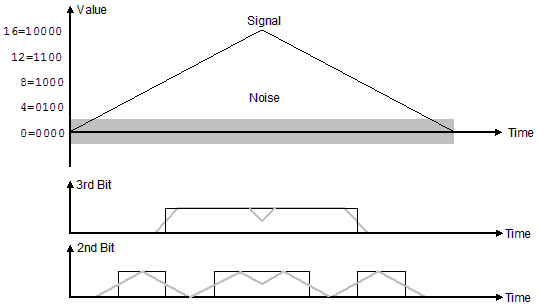
\includegraphics[height=2.5in]{Signal_and_Noise.png}
\captionof{figure}{
Effect of noise on bit values of a measured value.  The triangular wave signal and the added white noise are shown at top using the thin black line and the grey area, respectively.  The values are measured by a theoretical 4-bit Digital-to-Analog Converter in ideal condition, assuming LSB is the 0th bit.  The measured 3rd and 2nd bits without the added noise are shown using thin black lines, while the mean values of the measured 3rd and 2nd bits with the added noise are shown using thin grey lines.
This figure has been published previously \cite{Prev_Precision_Arithmetic}.
}
\label{fig: Signal_and_Noise}
\end{figure}

\begin{figure}[p]
\centering
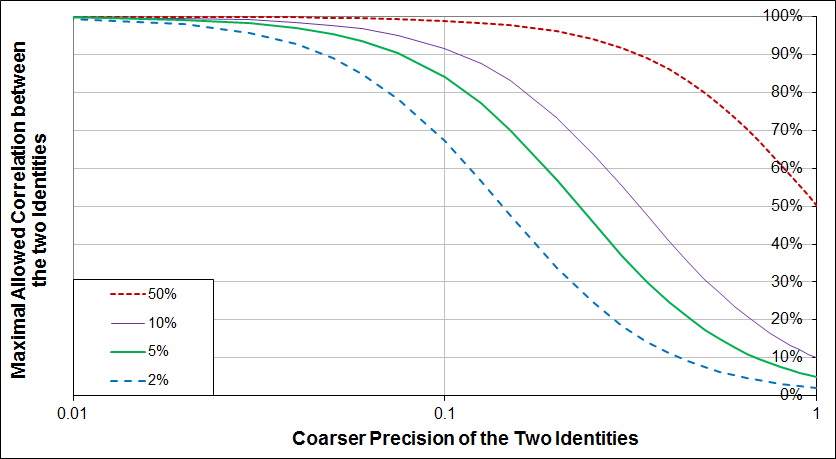
\includegraphics[height=2.5in]{Independent_Uncertainty_Assumption.png} 
\captionof{figure}{
Allowed maximal correlation between two values vs. input precisions and independence standard (as shown in legend) for the independence uncertainty assumption of variance arithmetic to be true.
This figure has been published previously \cite{Prev_Precision_Arithmetic}.
}
\label{fig: Independent_Uncertainty_Assumption}
\end{figure}

When there is a good estimation of the sources of uncertainty, the uncorrelated uncertainty assumption can be judged directly, e.g., if noise \cite{Statistical_Methods}\cite{Precisions_Physical_Measurements} is the major source of uncertainty, the uncorrelated uncertainty assumption is probably true.  
This criterion is necessary to ascertain repeated measurements of the same signal.   
Otherwise, the uncorrelated uncertainty assumption can be judged by the correlation and the respectively precision of two measurements.  

The correlated parts common to different measurements are regarded as signals, which can either be desired or unwanted.
Let $X$, $Y$, and $Z$ denote three mutually independent random variables \cite{Probability_Statistics} with variance $V(X)$, $V(Y)$ and $V(Z)$, respectively.  
Let $\alpha$ denote a constant.  
Let $Cov()$ denote the covariance function.  
Let $\gamma$ denote the correlation between $(X + Y)$ and $(\alpha X + Z)$. And let:
\begin{align}
\label{eqn: uncertainty ratio}
& \eta _{1} ^{2} \equiv \frac{V(Y)}{V(X)}; \eqspace
 \eta _{2} ^{2} \equiv \frac{V(Z)}{V(\alpha X)} =\frac{V(Z)}{\alpha ^{2} V(X)};  \\
\label{eqn: uncertainty correlation}
& \gamma =\frac{Cov(X+Y,\alpha X+Z)}{\sqrt{V(X+Y)} \sqrt{V(\alpha X+Z)}}  =\frac{\alpha /|\alpha |}{\sqrt{1+\eta _{1} ^{2} } \sqrt{1+\eta _{2} ^{2}}} \equiv \frac{\alpha /|\alpha |}{1+\eta ^{2}};
\end{align}
Formula \eqref{eqn: uncertainty correlation} gives the correlation $\gamma$ between two random variables, each of which contains a completely uncorrelated part and a completely correlated part $X$, with $\eta$ being the average ratio between these two parts.  
Formula \eqref{eqn: uncertainty correlation} can also be interpreted reversely: if two random variables are correlated by $\gamma$, each of them can be viewed hypothetically as containing a completely uncorrelated part and a completely correlated part, with $\eta$ being the average ratio between these two parts.

One special application of Formula \eqref{eqn: uncertainty correlation} is the correlation between a measured signal and its true signal, in which noise is the uncorrelated part between the two.  
Figure \ref{fig: Signal_and_Noise} shows the effect of noise on the most significant two bits of a 4-bit measured signal when $\eta=1/4$.  
Its top chart shows a triangular waveform between 0 and 16 as a black line, and a white noise between -2 and +2, using the grey area.  
The measured signal is the sum of the triangle waveform and the noise.  
The middle chart of Figure \ref{fig: Signal_and_Noise} shows the values of the 3rd digit of the true signal as a black line, and the mean values of the 3rd bit of the measurement as a grey line.  
The 3rd bit is affected by the noise during its transition between 0 and 1.  
For example, when the signal is slightly below 8, only a small positive noise can turn the 3rd digit from 0 to 1.  
The bottom chart of Figure \ref{fig: Signal_and_Noise} shows the values of the 2nd digit of the signal and the measurement as a black line and a grey line, respectively.  
Figure \ref{fig: Signal_and_Noise} clearly shows that the correlation between the measurement and the true signal is less at the 2nd digit than at the 3rd digit.  
Quantitatively, according to Formula \eqref{eqn: uncertainty correlation}:

\begin{enumerate}
\item  The overall measurement is 99.2\% correlated to the signal with $\eta=1/8$;
\item  The 3rd digit of the measurement is 97.0\% correlated to the signal with $\eta=1/4$;
\item  The 2nd digit of the measurement is 89.4\% correlated to the signal with $\eta=1/2$;
\item  The 1st digit of the measurement is 70.7\% correlated to the signal with $\eta=1$;
\item  The 0th digit of the measurement is 44.7\% correlated to the signal with $\eta=2$.
\end{enumerate}
The above conclusion agrees with the common experiences that, below the noise level of measured signals, noises rather than true signals dominate each digit.  

Similarly, while the correlated portion between two values has the same value at each bit of the two values, the ratio of the uncorrelated portion to the correlated portion increases by 2-fold for each bit down from MSB of the two values. 
Quantitatively, let $P$ denote the precision of an imprecise value, and let $\eta_{P}$ denote the ratio of the uncorrelated portion to the correlated portion at level of uncertainty; then $\eta_{P}$ increases with decreased $P$ according to Formula \eqref{eqn: uncertainty level}. 
According to Formula \eqref{eqn: uncertainty correlation}, if two significant values are overall correlated with $\gamma$, at the level of uncertainty the correlation between the two values decreases to $\gamma_P$ according to Formula \eqref{eqn: uncertainty correlation}.
\begin{align}
\label{eqn: uncertainty level}
& \eta_{P} = \frac{\eta}{P}, \eqspace P < 1; \\
\label{eqn: uncertainty correlation}
& \frac{1}{\gamma_{P}} - 1 = \left(\frac{1}{\gamma} -1\right) \frac{1}{P^2}, \eqspace P < 1;
\end{align}

Figure \ref{fig: Independent_Uncertainty_Assumption} plots the relation of $\gamma$ vs. $P$ for each given $\gamma_{P}$ in Formula \eqref{eqn: uncertainty correlation}.  
When $\gamma_{P}$ is less than a predefined maximal threshold (e.g., 2\%, 5\% or 10\%), the two values can be deemed uncorrelated to each other at the level of uncertainty.  
%If the two values are independent of each other at their uncertainty levels, their uncertainties are uncorrelated of each other.  
For each independence standard $\gamma_{P}$, there is a maximal allowed correlation between two values below which the uncorrelated uncertainty assumption of variance arithmetic holds.  
The maximal allowed correlation is a function of the larger precision of the two values according to Formula \eqref{eqn: uncertainty correlation}.  
Figure \ref{fig: Independent_Uncertainty_Assumption} shows that for two precisely measured values, their correlation $\gamma$ is allowed to be quite high.  
Thus, the uncertainty assumption uncertainty assumption has much weaker statistical requirement than the assumption for independence arithmetic, which requires the two values to be independent of each other.

It is tempting to add noise to otherwise unqualified values to make them satisfy the uncertainties uncertainty assumption.  
As an extreme case of this approach, if two values are constructed by adding noise to the same signal, they are 50\% correlated at the uncertainty level so that they will not satisfy the uncorrelated uncertainty assumption, which defines the upper bound for $\gamma_{P}$. 
\footnote{
The $50\%$ curve in Figure \ref{fig: Independent_Uncertainty_Assumption} defines the maximal possible correlations between any two measured signals. 
This other conclusion of Formula \eqref{eqn: uncertainty correlation} makes sense because the measurable correlation between two measurements should be limited by the precision of their measurements.
}


\subsection{Pure Rounding}

Empirically, the pure rounding error due to round-off is shown to be uniformly distributed between the half bit of the least significant bit of the siginficand \cite{Prev_Precision_Arithmetic}, whose probability density function is shown in Formula \eqref{eqn: rounding error 1/2 distribution}:
\begin{equation}
\label{eqn: rounding error 1/2 distribution}
P_{\frac{1}{2}}(x) \equiv 1, \eqspace  -1/2 \leq x \leq +1/2; 
\end{equation}



\subsection{Addition and Subtraction  \cite{Prev_Precision_Arithmetic}}

\begin{figure}
\centering
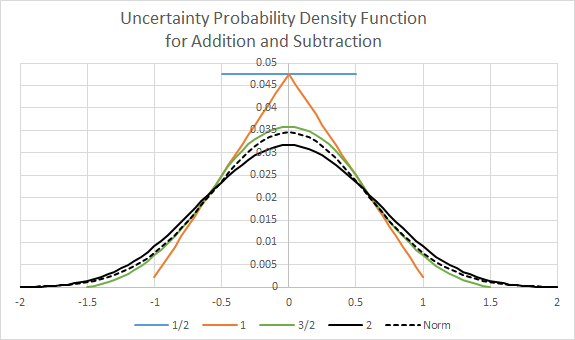
\includegraphics[height=2.5in]{Prec_Add_ErrDist.png} 
\captionof{figure}{
The probability distribution $P_{\frac{n}{2}}(x)$ of Formula \eqref{eqn:rounding error n/2 distribution}, assuming $P_{\frac{1}{2}}(x)$ is uniformly distributed between $(-1/2, +1/2)$.  
The legend shows $n$.
$P_{2}(x)$ is already close to the corresponding Gaussian distribution with the same mean and deviation, which is plotted in dash line of the same color.
This figure has been published previously \cite{Prev_Precision_Arithmetic}.
}
\label{fig: Prec_Add_Err_Dist}
\end{figure}


The uncorrelated uncertainty assumption suggests that the result bounding distribution density function of addition or subtraction is the convolution of the input density functions \cite{Probability_Statistics}.  
\begin{equation}
\label{eqn:rounding error n/2 distribution}
P_{\frac{n}{2}}(x) \equiv \int _{-\infty}^{+\infty}P_{\frac{1}{2}}(y)P_{\frac{n-1}{2}}(x-y)dy=\int _{-1/2}^{+1/2}P_{\frac{n-1}{2}}(x-y) dy,\eqspace n=2,3,4\dots;
\end{equation}
Figure \ref{fig: Prec_Add_Err_Dist} shows the probability distribution $P_{\frac{n}{2}}(x)$ of Formula \eqref{eqn:rounding error n/2 distribution}.  
$P_{2}(x)$ is already close to the corresponding Gaussian distribution with the same mean and deviation, which is plotted in dash line of the same color.

The Lyapunov form of the central limit theorem \cite{Probability_Statistics} states that if $X_i$ is a random variable with mean $\mu_i$ and variance $V_i$ for each $i$ among a series of $n$ mutually independent random variables, then with increased $n$, the sum $\sum\limits_{i}^{n} X_i$ converges in distribution to the Gaussian distribution with mean $\sum\limits_{i}^{n} \mu_i$ and variance $\sum\limits_{i}^{n} V_i$. Applying the central limit theorem to the addition and subtraction: 
\begin{itemize} 
\item $P_{n/2}(x)$ converges in distribution to a Gaussian distribution.

\item Figure \ref{fig: Prec_Add_Err_Dist} shows that such convergence to Gaussian distribution is very quick. 

\item The stable rounding error distribution is independent of any initial rounding error distribution. 
\end{itemize} 

Also due to the center-limit theorem, uncertainty in general is expected to be Gaussian distributed \cite{Statistical_Methods} \cite{Probability_Statistics}. 
The rounding error distribution is extended to describe uncertainty distribution in general.

For simplicity, define operator $\delta^2 f(x) \equiv (\delta f(x))^2$. 
Formula \eqref{eqn: addition and subtraction} gives the result variance of addition and subtraction surrounding $x \pm y$.
Formula \eqref{eqn: central limit theorem} gives the probability density function for $x \pm \delta x$ in general, in which $N()$ is the density function of the  normal distribution \cite{Probability_Statistics}.
Formula \eqref{eqn: central limit theorem} can be normalized as Formula \eqref{eqn: normalized distribution}.
\begin{align}
\label{eqn: addition and subtraction}
\delta^2 (x \pm y) &= (\delta x)^2 + (\delta y)^2; \\
\label{eqn: central limit theorem}
\rho(\tilde{x}, x, \delta x) & = \frac{1}{\delta x} N(\frac{\tilde{x} - x}{\delta x}); \\
\label{eqn: normalized distribution}
\tilde{z} \equiv \frac{\tilde{x} - x}{\delta x}:\eqspace & \rho(\tilde{x}, x, \delta x) d \tilde{x} = N(\tilde{z}) d \tilde{z};
\end{align}

Formula \eqref{eqn: addition and subtraction} is different from Formula \eqref{eqn: stat +} and \eqref{eqn: stat -}, because in variance arithmetic, the correlation between $x$ and $y$ does not contribute to the result distribution as far as the uncorrelated uncertainty assumption is satisfied.
It may show that Formula \eqref{eqn: stat +} and \eqref{eqn: stat -} are wrong statistically for the result uncertainty.



\subsection{A Variance Representation}

A variance arithmetic representation uses a pair of conventional floating-point numbers to represent the value $x$ and the variance $(\delta x)^2$ of an imprecise value $x \pm \delta x$.
When the uncertainty $\delta x$ is not specified initially:
\begin{itemize}
\item A conventional floating-point value is assumed to be imprecise in the least significant bit of its significand, and the error is assumed uniformly distributed within the bit.
The equivalent value of the bit is defined as the \emph{least significant value} \footnote{Together with least significant bit, it is a more indicative name for unit in the last place.}, so that the uncertainty is $1/\sqrt{3}$-fold of the least significant value.

\item An integer value within the range of $(-2^{53}, +2^{53})$ has 0 as its uncertainty.

\item An integer value outside the range of $(-2^{53}, +2^{53})$ is converted to a conventional floating-point value.
\end{itemize}


\subsection{Comparison}

\iffalse

Statistically the less relation between two imprecise values $x \pm \delta x$ and $y \pm (\delta y)^2$ is calculated by Formula \ref{eqn: x < y}:
\begin{align}
& z \equiv \frac{\tilde{y} - y}{\delta y}; \eqspace \tilde{y} = \delta y z + y; \\
& x - \Delta x < z \delta y + y < x + \Delta x; \\ & x - \Delta x - y < z \delta y < x + \Delta x - y \\
& - \Delta y < z \delta y < \Delta y; \\
p\left( x \pm (\delta x)^2 < y \pm (\delta y)^2 \right) & = 
  \int_{y - \Delta y}^{y + \Delta y} \rho(\tilde{y}, y, \delta y) 
    \int_{x - \Delta x}^{\tilde{y}} \rho(\tilde{x}, x, \delta x) d \tilde{x} \;d \tilde{y}; \\
& = \int_{y - \Delta y}^{y + \Delta y} \rho(\tilde{y}, y, \delta y) 
  \int_{-\frac{\Delta x}{\delta x}}^{\frac{\tilde{y} - x}{\delta x}} N(z) d z \;d \tilde{y}; \\
& = \int_{y - \Delta y}^{y + \Delta y} \rho(\tilde{y}, y, \delta y) 
      \frac{1}{2}(\frac{\tilde{y} - x}{\sqrt{2} \delta x}) - \zeta(\frac{-\Delta x}{\sqrt{2} \delta x})) \;d \tilde{y}; \\
& = \int_{\frac{\max(-\Delta y, x - \Delta x - y)}{\delta y}}^{\frac{\min(+\Delta y, x + \Delta x - y)}{\delta y}} 
      \frac{1}{2} \left(\zeta(\frac{z \delta y + y - x}{\sqrt{2} \delta x}) - \zeta(-\frac{\Delta x}{\sqrt{2} \delta x})\right) N(z) d z; \\
p\left( x \pm (\delta x)^2 > y \pm (\delta y)^2 \right) & =     
   \int_{\frac{\max(-\Delta y, x - \Delta x - y)}{\delta y}}^{\frac{\min(+\Delta y, x + \Delta x - y)}{\delta y}} 
      \frac{1}{2} \left(\zeta(+\frac{\Delta x}{\sqrt{2} \delta x}) - \zeta(\frac{z \delta y + y - x}{\sqrt{2} \delta x})\right) N(z) d z;
\end{align}
Formula \eqref{eqn: x < y} seems correct because it predicts $p(x \le y) = p(y \ge x)$:
\begin{align}
& \frac{d}{d \tilde{y}} \int_{-\infty}^{\tilde{y}} \rho(\tilde{x}, x, \delta x) d \tilde{x} = \rho(\tilde{y}, x, \delta x); \\
p(x< y) & = \int_{-\infty}^{+\infty} \rho(\tilde{y}, y, \delta y) \rho(\tilde{y}, x, \delta x) d \tilde{x} d \tilde{y} \\
& = \int_{-\infty}^{+\infty} \rho(\tilde{y}, y, \delta y) \;d \rho(\tilde{y}, x, \delta x) \\
& = 0 - \int_{-\infty}^{+\infty} \rho(\tilde{y}, x, \delta x) \;d \rho(\tilde{y}, y, \delta y) \\
& = \int_{-\infty}^{+\infty} \rho(\tilde{y}, x, \delta x) 
\int_{\tilde{y}}^{+\infty} \rho(\tilde{x}, y, \delta y) 
d \tilde{x} \;d \tilde{y} \\
& = \int_{-\infty}^{+\infty} \rho(\tilde{x}, x, \delta x) 
\int_{\tilde{x}}^{+\infty} \rho(\tilde{y}, y, \delta y) 
d \tilde{y} \;d \tilde{x}
\end{align}

Two imprecise values can be compared directly for less or greater relation when their ranges $(x - \Delta x, x + \Delta x)$ and $(y - \Delta y, y + \Delta y)$ do not overlap. 
Otherwise, statistically, Formula \eqref{eqn: x < y} and \eqref{eqn: x > y} gives the probability for less or greater relation between $x \pm (\delta x)^2 \le y \pm (\delta y)^2$, in which $\min()$ and $\max()$ are minimal and maximal functions, respectively.
Formula \eqref{eqn: no =} shows that two imprecise variable can not be equal statistically.
Let $x = y$, $\delta x = \delta y$ and $\Delta x = \Delta y$, Formula \eqref{eqn: x < y} and \eqref{eqn: x > y} shows that two conceptually equal imprecise values has $1/2$ chance to be one less than the other, and $1/2$ chance to be one more than the other.
Thus,
\begin{align}
\label{eqn: x < y}
& p\left( x \pm (\delta x)^2 < y \pm (\delta y)^2 \right) = 
  \int_{\frac{\max(-\Delta y, x - \Delta x - y)}{\delta y}}^{\frac{\min(+\Delta y, x + \Delta x - y)}{\delta y}} 
      \frac{1}{2} \left(\zeta(\frac{z \delta y + y - x}{\sqrt{2} \delta x}) - \zeta(-\frac{\Delta x}{\sqrt{2} \delta x})\right) N(z) d z; \\
\label{eqn: x > y}
& p\left( x \pm (\delta x)^2 > y \pm (\delta y)^2 \right) =     
  \int_{\frac{\max(-\Delta y, x - \Delta x - y)}{\delta y}}^{\frac{\min(+\Delta y, x + \Delta x - y)}{\delta y}} 
      \frac{1}{2} \left(\zeta(+\frac{\Delta x}{\sqrt{2} \delta x}) - \zeta(\frac{z \delta y + y - x}{\sqrt{2} \delta x})\right) N(z) d z; \\
\label{eqn: no =}
& p\left( x \pm (\delta x)^2 < y \pm (\delta y)^2 \right) + p\left( x \pm (\delta x)^2 > y \pm (\delta y)^2 \right) = 1;
\end{align}

\fi

Two imprecise values can be compared statistically using their difference.

When the value difference is zero, the two imprecise values are equal
\footnote{
Such definition of equality deviates from statistics.
In statistics, such two imprecise values has $50\%$ possibility to be less than or greater to each other but no chance to be equal to each other.
}.  

Otherwise, the standard z-method \cite{Probability_Statistics} is used to judge whether they are equal, or less or more than each other.
For example, the difference between $1.002 \pm 0.001$ and $1.000 \pm 0.002$ is $0.002 \pm 0.00224$, so that the z-value for the difference is $z = 0.002 / 0.00224$, and the probability for them to be not equal is $\xi(|z|) - \xi(-|z|) = 62.8\%$, in which $\xi(z)$ is the cumulative density function for normal distribution \cite{Probability_Statistics}.
If the threshold probability of not equality is $50\%$, $1.000 \pm 0.002 < 1.002 \pm 0.001$.
Instead of using the threshold probability, the bounding range for z can be used, such as $|z| \leq 0.67448975$ for the equivalent threshold probability of $50\%$.






\subsection{Multiplication}

\iffalse
\begin{align*}
0 \leq |x| - \Delta x, 0 \leq |y| - \Delta y: &\eqspace 
	(|x||y| - |x| \Delta y - |y| \Delta x + \Delta x \Delta y, |x||y| + |x| \Delta y + |y| \Delta x + \Delta x \Delta y) \\
&\eqspace \Delta xy = |x| \Delta y + |y| \Delta x; \\
|x| - \Delta x \leq 0 \leq |y| - \Delta y: &\eqspace 
    (|x||y| + |x| \Delta y - |y| \Delta x - \Delta x \Delta y, |x||y| + |x| \Delta y + |y| \Delta x + \Delta x \Delta y) \\
&\eqspace \Delta xy = |y| \Delta x + \Delta x \Delta y; \\
|x| - \Delta x \leq 0, \; |y| - \Delta y \leq 0: &\eqspace
	(|x||y| + |x| \Delta y - |y| \Delta x - \Delta x \Delta y, |x||y| + |x| \Delta y + |y| \Delta x + \Delta x \Delta y) \\
&\eqspace \Delta xy = |y| \Delta x + \Delta x \Delta y;
\end{align*}
But the range needs to be centered at $|x||y|$.
\fi

The result variance of multiplying $x \pm \delta x$ by a precise value $y$ is $ y^2 \delta^2 x$ \cite{Probability_Statistics}.
The result of multiplying $0 \pm \delta x$ by $0 \pm \delta y$ is a normal production distribution \cite{Probability_Statistics}, which is centered at 0 with variance $(\delta x)^2 (\delta y)^2$.
The general multiplication can be decomposed as Formula \eqref{eqn: multiplication decomposed}, which leads to Formula \eqref{eqn: multiplication}  \cite{Prev_Precision_Arithmetic}.
\begin{align}
\label{eqn: multiplication decomposed}
& (x \pm \delta x) \times (y \pm \delta y) = (x + (0 \pm \delta x)) \times (y + (0 \pm \delta y)); \\
\label{eqn: multiplication}
\delta^2 (x y) &= x^2 (\delta^2 y) + y^2 (\delta^2 x) + (\delta^2 x)(\delta^2 y);
\end{align}

Formula \eqref{eqn: multiplication} is identical to Formula \eqref{eqn: stat *} for statistical propagation of uncertainty except their cross term, representing difference in their statistical requirements, respectively.  
Formula \eqref{eqn: multiplication} is simpler and more elegant than Formula \eqref{eqn: interval *} for interval arithmetic multiplication.  
The result of Formula \eqref{eqn: float num calc} calculated by variance arithmetic is $2 \pm 2\sqrt{5}$.
It is $2 \pm 9$ for interval arithmetic \cite{Worst_Case_Error_Bounds}.




\subsection{Uncertainty Distribution}

\iffalse

To solve for mode:
\begin{align*}
& \rho(\tilde{y}, y, \delta y) = \frac{d \tilde{z}}{d \tilde{y}} N(\tilde{z});
\eqspace \tilde{z} = \frac{f^{-1}(\tilde{y}) - x}{\delta x}; \\
& 0 = \frac{d \rho(\tilde{y}, y, \delta y)}{d \tilde{y}} = \frac{d^2 \tilde{z}}{d \tilde{y}^2} N(\tilde{z}) - \frac{d \tilde{z}}{d \tilde{y}} N(\tilde{z}) \tilde{z}; \\
& \frac{d^2 \tilde{z}}{d \tilde{y}^2} = \frac{d \tilde{z}}{d \tilde{y}} \tilde{z}; \eqspace \tilde{z} = \frac{f^{-1}(\tilde{y}) - x}{\delta x};
\end{align*}

The exponential function:
\begin{align*}
f(x) = e^x:& \eqspace 
\tilde{z} = \frac{\log(\tilde{y}) - x}{\delta x}, \eqspace 
\frac{d \tilde{z}}{d \tilde{y}} = \frac{1}{\tilde{y} \delta x} = \frac{1}{\frac{d}{d \tilde{z}} e^{x + \tilde{z} \delta x}}; \eqspace \\
\frac{d \tilde{z}}{d \tilde{y}} N(\tilde{z})
&= e^{-\log(\tilde{y})} \frac{1}{\sqrt{2\pi} \delta x} e^{-\frac{(\log(\tilde{y}) - x)^2}{2 \delta^2 x}}
 = \frac{1}{\sqrt{2\pi} \delta x} e^{-\frac{(\log(\tilde{y}) - x)^2 + 2 \log(\tilde{y}) \delta^2 x }{2 \delta^2 x}} \\
& = \frac{1}{\sqrt{2\pi} \delta x} e^{-\frac{(\log(\tilde{y}) - (x - \delta^2 x))^2 + 2 x \delta^2 x - (\delta^2 x)^2 }{2 \delta^2 x}}
 = N(\frac{\log(\tilde{y}) - (x - \delta^2 x)}{\delta x}) e^{-x + \frac{\delta^2 x}{2}}; \\
& 0 = \tilde{z} e^{x + \tilde{z} \delta x} + (\delta x) e^{x + \tilde{z} \delta x}; \eqspace
 \tilde{z} = -(\delta x) = \frac{1}{\delta x}(x - (\delta x)^2 - x);
\end{align*}

The log function $f(x) = \ln(x)$:
\begin{align*}
& \tilde{z} = \frac{e^{\tilde{y}} - x}{\delta x}; \eqspace 
\frac{d \tilde{z}}{d \tilde{y}} = \frac{1}{\delta x} e^{\tilde{y}} = \frac{1}{\delta x} (x + \tilde{z} \delta x)
 = \frac{1}{\frac{d}{d \tilde{z}} \ln(x + \tilde{z} \delta x)}; \\
& \frac{1}{\delta x} e^{\tilde{y}} = (\frac{1}{\delta x} e^{\tilde{y}})^2 \frac{e^{\tilde{y}} - x}{\delta x}; \eqspace 
(e^{\tilde{y}})^2 - x e^{\tilde{y}} - \delta^2 x = 0; \\
e^{\tilde{y}_m} &= \frac{x + \sqrt{x^2 + 4 \delta^2 x}}{2}; \\
& \eqspace 0 = \frac{\tilde{z}}{x + \tilde{z} \delta x} - (\delta x) \frac{1}{(x + \tilde{z} \delta x)^2}; \eqspace
0 = (\delta x) \tilde{z}^2 + x \tilde{z} - (\delta x); \\
& \tilde{z} = \frac{1}{\delta x}(\frac{x + \sqrt{x^2 + 4 (\delta x)^2}}{2} - x);
\end{align*}

The power mode $f(x) = x^{\frac{1}{p}}$:
\begin{align*}
& \tilde{z} = \frac{\tilde{y}^p - x}{\delta x}; \eqspace 
\frac{d \tilde{z}}{d \tilde{y}} = \frac{1}{\delta x} p \tilde{y}^{p-1}; \\
& \frac{1}{\delta x} p (p - 1) \tilde{y}^{p-2} = (\frac{1}{\delta x} p \tilde{y}^{p-1})^2 \frac{\tilde{y}^p - x}{\delta x}; \\
& \tilde{y}^{2p} - x \tilde{y}^{p} - \frac{p - 1}{p} \delta^2 x = 0; \\
\tilde{y}_m^p &= \frac{1}{2} (x + \sqrt{x^2 + 4 \frac{p - 1}{p} \delta^2 x}); \\
& 0 = c (x + \tilde{z} \delta x)^{c-1} \tilde{z} + c (c-1) \delta x (x + \tilde{z} \delta x)^{c-2}; \eqspace
0 = (\delta x) \tilde{z}^2 + x \tilde{z} + (c - 1) (\delta x); \\
& \tilde{z}_m = \frac{1}{\delta x}(\frac{x + \sqrt{x^2 - 4(c-1)(\delta x)^2}}{2} - x); \eqspace 
f^{-1}(\tilde{y}_m) = \frac{x + \sqrt{x^2 - 4(c-1)(\delta x)^2}}{2}; \\
p = 2:& \eqspace \frac{d \tilde{z}}{d \tilde{y}} = \frac{1}{\delta x} 2 \tilde{y}; \eqspace 
  \tilde{y}_m^{\frac{1}{2}} = \frac{1}{2} \left( x + \sqrt{x^2 + 2 \delta^2 x} \right); \\
p = 3:& \eqspace \frac{d \tilde{z}}{d \tilde{y}} = \frac{1}{\delta x} 3 \tilde{y}^2; \eqspace  
  \tilde{y}_m^{\frac{1}{3}} = \frac{1}{2} \left( x \pm \sqrt{x^2 + \frac{8}{3} \delta^2 x} \right); \\
p = 1/2:& \eqspace \frac{d \tilde{z}}{d \tilde{y}} = \frac{1}{\delta x} \frac{1}{2} \tilde{y}^{-\frac{1}{2}}; \eqspace 
  \tilde{y}_m^2 = \frac{1}{2} \left( x + \sqrt{x^2 - 4 \delta^2 x} \right); \\
p = 1/3:& \eqspace \frac{d \tilde{z}}{d \tilde{y}} = \frac{1}{\delta x} \frac{1}{3} \tilde{y}^{-\frac{2}{3}}; \eqspace
  \tilde{y}_m^2 = \frac{1}{2} \left( x \pm \sqrt{x^2 - 8 \delta^2 x} \right); \\
p = -1:& \eqspace \frac{d \tilde{z}}{d \tilde{y}} = - \frac{1}{\delta x} \tilde{y}^{-2}; \eqspace 
  \tilde{y}_m^{-1} = \frac{1}{2} \left( x + \sqrt{x^2 + 8 \delta^2 x} \right); 
\end{align*}


The distribution difference:
\begin{align*}
&\nu = \frac{x - f^{-1}(\tilde{y}_m)}{\delta x}: \eqspace 
 N(\frac{f^{-1}(\tilde{y}) - f^{-1}(\tilde{y}_m)}{\delta x} )
 = N(\tilde{z} + \nu) = N(\tilde{z}) e^{-\tilde{z} \nu} e^{-\frac{1}{2} \nu^2}; \\
\eta &\equiv \int |\varrho(\tilde{y}, y, \delta y) - \rho(\tilde{y}, y, \delta y)| d \tilde{y}
 =  \int |\rho(f^{-1}(\tilde{y}), f^{-1}(\tilde{y_m}), \delta x) - \rho(f^{-1}(\tilde{y}), x, \delta x)| d f^{-1}(\tilde{y}) \\
&= \int |N(\tilde{z} + \nu) - N(\tilde{z})| d \tilde{z} 
 = \int |e^{-\frac{1}{2} \nu^2} e^{-\tilde{z} \nu} - 1| N(\tilde{z}) d \tilde{z}; \\
&= | \int |\sum_{m=0}^{\infty} \frac{(-\nu^2)^m}{2^m m!} \sum_{n=0}^{\infty} \frac{(-\nu)^n}{n!} \tilde{z}^n - 1| 
   N(\tilde{z}) d \tilde{z} | \\
&= | \int \left(\sum_{m=1}^{\infty} \frac{(-\nu^2)^m}{2^m m!} \sum_{n=1}^{\infty} \frac{(-\nu)^n}{n!} \tilde{z}^n
  - \frac{1}{2} \nu^2 - \nu \tilde{z} \right) N(\tilde{z}) d \tilde{z} | \\
&= \frac{1}{2} \nu^2 - \sum_{m=1}^{\infty} \frac{(-\nu^2)^m}{2^m m!} \sum_{n=1}^{\infty} \frac{\nu^{2n}}{2^n n!}
 = \frac{1}{2} \nu^2 - \sum_{m=2}^{\infty} \sum_{n=1}^{m-1} \frac{(-1)^m}{2^m (m - n)! n!} \nu^{2m} \\
&\simeq \frac{1}{2} \nu^2 - \frac{1}{4} \nu^4 + \frac{1}{8} \nu^6 - \frac{7}{192} \nu^8;
\end{align*}
When $f(x)=x^c$:
\begin{align*}
\nu &= \frac{x - \frac{1}{2} (x + \sqrt{x^2 + (1 - c) 4 \delta^2 x})}{\delta x} = \frac{1 - \sqrt{1 + (1 - c) 4 P(x)^2}}{2 P(x)} \\
&= - \sum_{m=1} \frac{(1 - c)^m (2P(x))^{2m - 1}}{m!} \prod_{n=1}^{m} \frac{\frac{3}{2} -n}{n} \\
&\simeq -(1 - c) P(x) + \frac{1}{4} (1 - c)^2 P(x)^3 - \frac{1}{4} (1 - c)^3 P(x)^5; \\
\eta &= \frac{1}{2} (1-c)^2 P(x)^2 - \frac{1}{4} (1-c)^3 (2-c) P(x)^4 + 1/8 (1-c)^4 (c^2-4c+7) P(x)^6
\end{align*}

\fi

\begin{figure}[p]
\centering
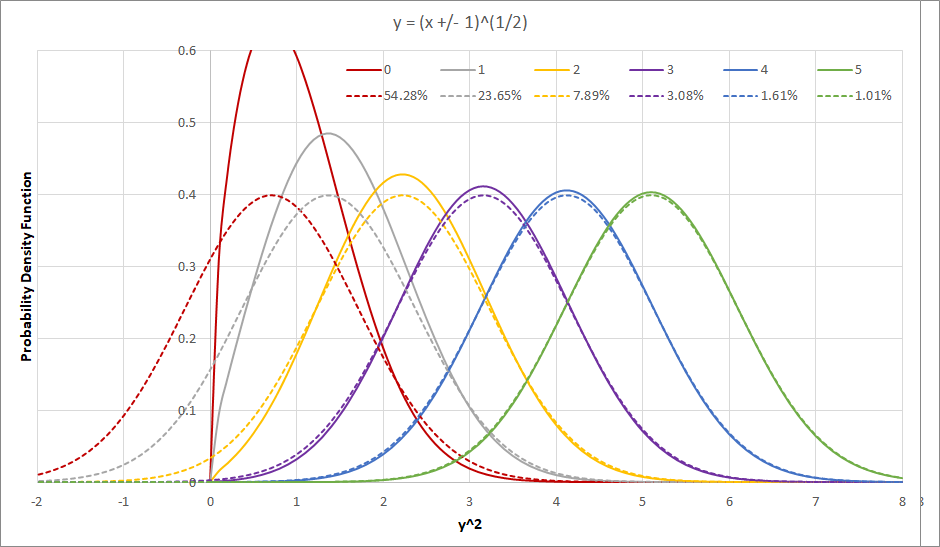
\includegraphics[height=2.5in]{Square_Root_Distribution.png} 
\captionof{figure}{
The probability density function for $\tilde{y} = \sqrt{x \pm 1}$, for different $x$ as shown in the legend. 
The $x$-axis is scaled as $\tilde{y}^2$.
Each probability density function $\rho(\tilde{x})$ in solid line is compared with a Gaussian distribution $\varrho(\tilde{x})$ of the same mode and the same deviation in the dash line of the same color.
The legend for the Gaussian distribution shows the value of Gaussian difference in percentage.
}
\label{fig: Square_Root_Distribution}
\end{figure}

\begin{figure}[p]
\centering
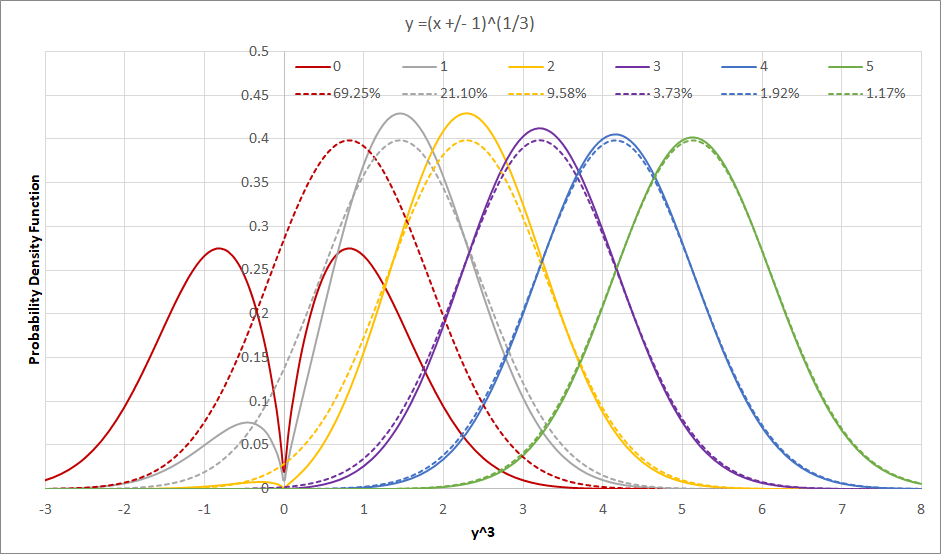
\includegraphics[height=2.5in]{Cubic_Root_Distribution.png} 
\captionof{figure}{
The probability density function for $\sqrt[3]{x \pm 1}$, for different $x$ as shown in the legend. 
The $y$-axis is scaled as $\tilde{y}^3$.
Each probability density function $\rho(\tilde{x})$ in solid line is compared with a Gaussian distribution $\varrho(\tilde{x})$ of the same mode and the same deviation in the dash line of the same color.
The legend for the Gaussian distribution shows the value of Gaussian difference in percentage.
}
\label{fig: Cubic_Root_Distribution}
\end{figure}

\begin{figure}[p]
\centering
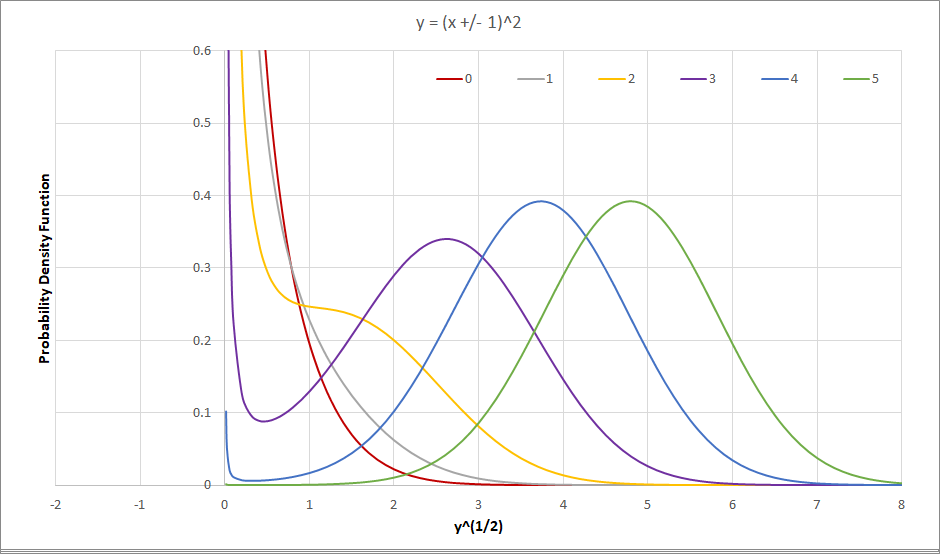
\includegraphics[height=2.5in]{Square_Distribution.png} 
\captionof{figure}{
The probability density function for $(x \pm 1)^2$, for different $x$ as shown in the legend. 
The $y$-axis is scaled as $\sqrt{\tilde{y}}$.
Some probability density function $\rho(\tilde{x})$ in solid line is compared with a Gaussian distribution $\varrho(\tilde{x})$ of the same mode and the same deviation in the dash line of the same color.
The legend for the Gaussian distribution shows the value of Gaussian difference in percentage.
}
\label{fig: Square_Distribution}
\end{figure}

\begin{figure}[p]
\centering
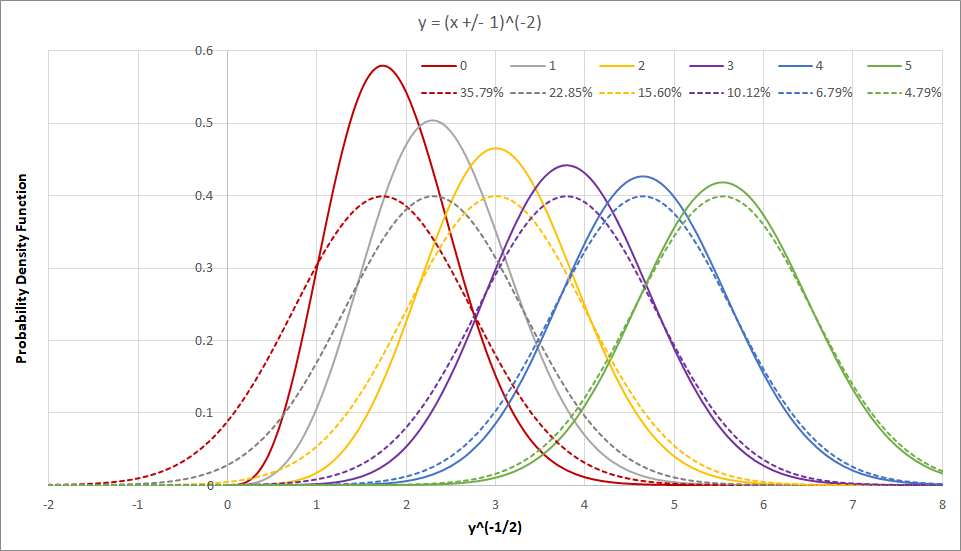
\includegraphics[height=2.5in]{Inverse_Square_Distribution.png} 
\captionof{figure}{
The probability density function for $1/(x \pm 1)^2$, for different $x$ as shown in the legend. 
The $y$-axis is scaled as $1/\sqrt{\tilde{y}}$.
The probability density function $\rho(\tilde{x})$ in solid line is compared with a Gaussian distribution $\varrho(\tilde{x})$ of the same mode and the same deviation in the dash line of the same color.
The legend for the Gaussian distribution shows the value of Gaussian difference in percentage.
}
\label{fig: Inverse_Square_Distribution}
\end{figure}


Let $\tilde{y} = f(\tilde{x})$ be a strictly monotonic function, so that $\tilde{x} = f^{-1}(\tilde{y})$ exist.
Formula \eqref{eqn: function distribution} is the uncertainty distribution density function \cite{Statistical_Methods}.
In Formula \eqref{eqn: function distribution} \cite{Statistical_Methods}, the same distribution can be expressed in either $\tilde{x}$ or $\tilde{y}$ or $\tilde{z}$ , which are different representations of the same underlying random variable.
Using Formula \eqref{eqn: function distribution}, Formula \eqref{eqn: exp distribution}, \eqref{eqn: log distribution}, and \eqref{eqn: power distribution} give the $\rho(\tilde{y}, y, \delta y)$ for $e^x$, $\ln(x)$, and $x^c$, respectively.
\begin{align}
\label{eqn: function distribution}
N(\tilde{z}) d \tilde{z} = \rho(\tilde{x}, x, \delta x) d\tilde{x} &= \rho(f^{-1}(\tilde{y}), x, \delta x) \frac{d\tilde{x}}{d\tilde{y}} d\tilde{y} 
= \rho(\tilde{y}, y, \delta y) d\tilde{y}; \\
\label{eqn: exp distribution}
y = e^x: &\; \rho(\tilde{y}, y, \delta y) = \frac{1}{\tilde{y}} \frac{1}{\delta x} N(\frac{\log(\tilde{y}) - x}{\delta x}); \\
\label{eqn: log distribution}
y = \ln(x): &\; \rho(\tilde{y}, y, \delta y) = e^{\tilde{y}} \frac{1}{\delta x} N(\frac{e^{\tilde{y}} - x}{\delta x}); \\
\label{eqn: power distribution}
y = x^c: &\; \rho(\tilde{y}, y, \delta y) = c \tilde{y}^{\frac{1}{c}-1} \frac{1}{\delta x} N(\frac{\tilde{y}^\frac{1}{c} - x}{\delta x}); 
\end{align}
Using Formula \eqref{eqn: function distribution}, Formula \eqref{eqn: distribution mode} gives the equation for the mode of the result distribution, whose solutions $f^{-1}(\tilde{y}_m)$ for $e^x$, $\ln(x)$, and $x^c$ are Formula \eqref{eqn: exp mode}, \eqref{eqn: log mode}, and \eqref{eqn: power mode} respectively.
\begin{align}
\label{eqn: distribution mode}
\eqspace \tilde{z} = \frac{f^{-1}(\tilde{y}) - x}{\delta x}: &\eqspace \frac{d^2 \tilde{z}}{d \tilde{y}^2} = \frac{d \tilde{z}}{d \tilde{y}} \tilde{z}; \\
\label{eqn: exp mode}
\tilde{y} = e^{\tilde{x}}: &\eqspace \ln(\tilde{y}_m) = x - (\delta x)^2; \\
\label{eqn: log mode}
\tilde{y} = \ln(\tilde{x}): &\eqspace e^{\tilde{y}_m} = \frac{x + \sqrt{x^2 + 4 (\delta x)^2}}{2}; \\
\label{eqn: power mode}
\tilde{y} = \tilde{x}^c: &\eqspace (\tilde{y}_m)^{1/c} = \frac{x + \sqrt{x^2 - 4(c-1)(\delta x)^2}}{2};
\end{align}

The \emph{Gaussian difference} of $\rho(f^{-1}(\tilde{y}), x, \delta x)$ is calculated as $\int_{-\infty}^{+\infty} |\rho(f^{-1}(\tilde{y}), x, \delta x) - \varrho(\tilde{y})| d \tilde{y}$ in which $\varrho(\tilde{y})$ is the Gaussian distribution of the same mode and the same deviation $\delta x$.
A Gaussian difference of 0 means a perfect Gaussian.

Viewed in the $f^{-1}(\tilde{y})$ coordinate, $\rho(\tilde{y}, y, \delta y)$ is Gaussian modulated by $\frac{d\tilde{x}}{d\tilde{y}} = 1/f^{(1)}_x$.
A \emph{zero} of the uncertainty distribution happens when $f^{(1)}_x=\infty \rightarrow \rho(\tilde{y}, y, \delta y) = 0$, while a \emph{pole} happens when $f^{(1)}_x=0 \rightarrow \rho(\tilde{y}, y, \delta y) = \infty$.
Zeros and poles have different impacts on the properties of of the uncertainty distributions.

If $y=f(x)$ is a linear transform of $x$, $f^{(1)}_x$ is a constant, and $\rho(\tilde{y}, y, \delta y)$ is known to be Gaussian \cite{Probability_Statistics}.
From another perspective, a linear transformation generates neither zero nor pole according to Formula \eqref{eqn: function distribution}.

Figure \ref{fig: Square_Root_Distribution} shows the probability density function for $\sqrt{x \pm 1}$ according to Formula \eqref{eqn: power distribution}, which has a zero at $x=0$.
Each probability density function $\rho(\tilde{x})$ in solid line is compared with a normal distribution $\varrho(\tilde{x})$ of the same mode in dash line of the same color.

Figure \ref{fig: Cubic_Root_Distribution} shows the probability density function for $\sqrt[3]{x \pm 1}$ according to Formula \eqref{eqn: power distribution}, which also has a zero at $x=0$.
Compared with $\sqrt{x \pm 1}$, $\sqrt[3]{x \pm 1}$ distributes on $\tilde{y} < 0$ also, so that the uncertainty distributions for $\sqrt[3]{0 \pm 1}$ has two equal peaks instead of one larger peak on the positive side only for $\sqrt{x \pm 1}$.

Figure \ref{fig: Square_Distribution} shows the probability density function for $(x \pm 1)^2$ according to Formula \eqref{eqn: power distribution}, which has a pole at $x=0$.
The uncertainty distributions for $(0 \pm 1)^2$ and $(1 \pm 1)^2$ deviate significantly from Gaussian, while the uncertainty distributions for $(4 \pm 1)^2$ and $(5 \pm 1)^2$ look Gaussian but each still with an infinitive but narrower peak at $\tilde{y} = 0$.
According to Formula \eqref{eqn: power mode}, both $(0 \pm 1)^2$ and $(1 \pm 1)^2$ have no mode.
$(0 \pm 1)^2$ is the $\chi^2$ distribution \cite{Statistical_Methods}.

Figure \ref{fig: Inverse_Square_Distribution} shows the probability density function for $1/(x \pm 1)^2$ according to Formula \eqref{eqn: power distribution}, which has a zero at $x=0$.
Figure \ref{fig: Inverse_Square_Distribution} looks more like Figure \ref{fig: Square_Root_Distribution} than Figure \ref{fig: Square_Distribution}, showing that pole or zero determines the properties of uncertainty distributions.

In all the figures, the probability density function in the $\tilde{z}$ representation becomes more Gaussian-like when the mode of the distributions is further away from either zero or pole.
Such observation leads to the following Taylor method to calculate the result variances when the distribution is nearly Gaussian in the $\tilde{z}$ representation.
 



\subsection{Analytic Functions}

\iffalse

\begin{align*}
& \tilde{y} = f(x + \tilde{z} \delta x) = \sum_{n=0}^{\infty} \frac{f^{(n)}_x}{n!} \tilde{z}^n (\delta x)^n; \\
\overline{f(x)} &\equiv \int \tilde{y} \rho(\tilde{y}, y, \delta y) d \tilde{y}
 = \int \sum_{n=0}^{\infty} \frac{f^{(n)}_x}{n!} \tilde{z}^n (\delta x)^n N(\tilde{z}) d \tilde{z}
 = \sum_{n=0}^{\infty} \frac{f^{(n)}_x}{n!} (\delta x)^{n} \int \tilde{z}^n N(\tilde{z}) d \tilde{z} \\
&= \sum_{n=0}^{\infty} \frac{f^{(n)}_x}{n!} (\delta x)^{n} \zeta(n)
 = \sum_{n=0}^{\infty} \frac{f^{(2n)}_x}{(2n)!} (\delta x)^{2n} \zeta(2n); \\
\delta^2 f(x) &\equiv \int \tilde{y}^2 \rho(\tilde{y}, y, \delta y) d \tilde{y} - \overline{f(x)}^2
 = \int (\sum_{n=0}^{\infty} \frac{f^{(n)}_x}{n!} \tilde{z}^n (\delta x)^n)^2 N(\tilde{z}) d \tilde{z} - \overline{f(x)}^2 \\
&= \sum_{n=0}^{\infty} \sum_{j=0}^{2n} \frac{f^{(j)}_x}{j!} \frac{f^{(2n-j)}_x}{(2n-j)!} (\delta x)^{2n} \zeta(2n)
 - \sum_{n=0}^{\infty} \sum_{j=0}^{n} \frac{f^{(2j)}_x}{(2j)!} \frac{f^{(2n-2j)}_x}{(2n-2j)!} (\delta x)^{2n} \zeta(2j) \zeta(2n - 2j) \\
&= \sum_{n=1}^{\infty} (\delta x)^{2n} ( \zeta(2n) \sum_{j=1}^{2n-1} \frac{f^{(j)}_x}{j!} \frac{f^{(2n-j)}_x}{(2n-j)!}
  - \sum_{j=1}^{n-1} \frac{f^{(2j)}_x \zeta(2j)}{(2j)!} \frac{f^{(2n-2j)}_x \zeta(2n - 2j)}{(2n-2j)!} \\
&\eqspace + 2 \zeta(2n) f(x) \frac{f^{(2n)}_x}{(2n)!} - 2 f(x) \frac{f^{(2n)}_x \zeta(2n)}{(2n)!}) \\
&= \sum_{n=1}^{\infty} (\delta x)^{2n} \left( \zeta(2n) \sum_{j=1}^{2n-1} \frac{f^{(j)}_x}{j!} \frac{f^{(2n-j)}_x}{(2n-j)!}
  - \sum_{j=1}^{n-1} \frac{f^{(2j)}_x \zeta(2j)}{(2j)!} \frac{f^{(2n-2j)}_x \zeta(2n - 2j)}{(2n-2j)!} \right) \\
&= (\delta x)^2 (f^{(1)}_x)^2 + (\delta x)^4 \left(f^{(1)}_x f^{(3)}_x + \frac{1}{2} (f^{(2)}_x)^2 \right) \\
&\eqspace + (\delta x)^6 \left(\frac{1}{4} f^{(1)}_x f^{(5)}_x + \frac{1}{2} f^{(2)}_x f^{(4)}_x + \frac{5}{12} (f^{(3)}_x)^2 \right) + o((\delta x)^8); \\
\delta^2 f(x) &= \sum_{n=1}^{\infty} (\delta x)^{2n} \zeta(2n) \sum_{j=0}^{2n} \frac{f^{(j)}_x}{j!} \frac{f^{(2n-j)}_x}{(2n-j)!} - \overline{f(x)}^2 \\
  &= \sum_{n=1}^{\infty} (\delta x)^{2n} \frac{\zeta(2n)}{(2n)!} (f(x)^2)^{(2n)}_x - \overline{f(x)}^2; \\
  &= (\delta x)^2 (f(x) f^{(2)}_x + (f^{(1)}_x)^2 - f(x) f^{(2)}_x) \\
  &\eqspace + (\delta x)^4 (\frac{1}{4} f(x) f^{(4)}_x + f^{(1)}_x f^{(3)}_x + \frac{3}{4} (f^{(2)}_x)^2 - \frac{1}{4} f(x) f^{(4)}_x - \frac{1}{4} (f^{(2)}_x)^2)    \\
  & = (\delta x)^2 (f^{(1)}_x)^2 + (\delta x)^4 (f^{(1)}_x f^{(3)}_x + \frac{1}{2} (f^{(2)}_x)^2) + o((\delta x)^6);  \\
\overline{f(x)} &= f(x) + (\delta x)^2 \frac{1}{2} f^{(2)}_x + (\delta x)^4 \frac{1}{8} f^{(4)}_x + o((\delta x)^6); \\
f(x + \tilde{x})^2 &= f(x)^2 + \frac{\tilde{x}}{1!} (2 f(x) f^{(1)}_x) + \frac{\tilde{x}^2}{2!} (2 f(x) f^{(2)}_x + 2 (f^{(1)}_x)^2) \\
&\eqspace + \frac{\tilde{x}^3}{3!} (2 f(x) f^{(3)}_x + 6 f^{(1)}_x f^{(2)}_x) 
     + \frac{\tilde{x}^4}{4!} (2 f(x) f^{(4)}_x + 8 f^{(1)}_x f^{(3)}_x + 6 (f^{(2)}_x)^);
\end{align*}


\begin{align*}
\int^z \tilde{z}^{n} e^{-\frac{\tilde{z}^2}{2}} d \tilde{z} &= -\int^z \tilde{z}^{n - 1} e^{-\frac{\tilde{z}^2}{2}} d {-\frac{\tilde{z}^2}{2}}
  = - z^{n-1} e^{-\frac{z^2}{2}} + (n-1) \int^z \tilde{z}^{n-2} e^{-\frac{\tilde{z}^2}{2}} d \tilde{z} \\
 &= - z^{n-1} e^{-\frac{z^2}{2}} - (n-1) z^{n-3} e^{-\frac{z^2}{2}} 
  + (n-1) (n-3) \int^z \tilde{z}^{n -3} e^{-\frac{\tilde{z}^2}{2}} d \tilde{z} \\
 &= - \frac{(n-1)!!}{(n-1)!!} z^{n-1} e^{-\frac{z^2}{2}} - \frac{(n-1)!!}{(n-3)!!} z^{n-3} e^{-\frac{z^2}{2}} 
  + (n-1) (n-3) \int \tilde{z}^{n -3} e^{-\frac{\tilde{z}^2}{2}} e^{-\frac{\tilde{z}^2}{2}} d \tilde{z}; \\
\int^z \tilde{z}^{2n + 1} N(\tilde{z}) d \tilde{z} &= - (2n)!! N(z) \sum_{j=0}^{n} \frac{z^{2j}}{(2j)!!}; \\
\int^z \tilde{z}^{2n + 2} N(\tilde{z}) d \tilde{z} &= (2n + 1)!! \xi(z) - (2n + 1)!! N(z) \sum_{j=0}^{n} \frac{z^{2j + 1}}{(2j + 1)!!};
\end{align*}

\begin{align*}
N(\sigma) \sum_{j=0}^{n} \frac{\sigma^{2j+1}}{(2j+1)!!} 
 & = N(\sigma) \left( \sqrt{\frac{\pi}{2}} e^{\frac{\sigma^2}{2}} (2 \xi(\sigma) - 1) - \sum_{j=n+1}^{\infty} \frac{\sigma^{2j+1}}{(2j+1)!!} \right) \\
 &= \xi(\sigma) - \frac{1}{2} - N(\sigma) \sum_{j=n+1}^{\infty} \frac{\sigma^{2j+1}}{(2j+1)!!} 
  = \xi(\sigma) - \frac{1}{2} - N(\sigma) \sigma^{2n} \sum_{j=1}^{\infty} \frac{\sigma^{2j+1}}{(2n + 2j+1)!!}; \\
\int_{+\sigma}^{+\infty} \tilde{z}^{2n + 2} N(\tilde{z}) d \tilde{z} 
 &= (2n+1)!! - (2n+1)!! \left(\xi(\sigma) - N(\sigma) \sum_{j=0}^{n} \frac{\sigma^{2j + 1}}{(2j + 1)!!} \right) \\
 &= (2n+1)!! - (2n+1)!! \left(\frac{1}{2} + N(\sigma) \sigma^{2n} \sum_{j=1}^{\infty} \frac{\sigma^{2j+1}}{(2n + 2j+1)!!} \right) \\
 &= \frac{1}{2} (2n+1)!! - N(\sigma) \sigma^{2n} \sum_{j=1}^{\infty} \sigma^{2j+1} \frac{(2n+1)!!}{(2n + 2j+1)!!}; \\
\int_{-\infty}^{-\sigma} \tilde{z}^{2n + 2} N(\tilde{z}) d \tilde{z} &= \int_{+\sigma}^{+\infty} \tilde{z}^{2n + 2} N(\tilde{z}) d \tilde{z}; \\
\int_{-\sigma}^{+\sigma} \tilde{z}^{2n + 2} N(\tilde{z}) d \tilde{z} &= 2 N(\sigma) \sigma^{2n} \sum_{j=1}^{\infty} \sigma^{2j+1} \frac{(2n+1)!!}{(2n + 2j+1)!!}; \\
 &= 2 N(\sigma) \sigma^{2(n+1)-2} \sum_{j=1}^{\infty} \sigma^{2(j-1) + 3} \frac{(2(n+1)-1)!!}{(2(n+1) + 2(j-1) + 1)!!};
\end{align*}

\begin{align*}
\zeta(2n) &= \int_{-\sigma}^{+\sigma} \tilde{z}^{2n} N(\tilde{z}) d \tilde{z} = 2 N(\sigma) \sigma^{2n} \sum_{j=0}^{\infty} \sigma^{2j+1} \frac{(2n-1)!!}{(2j + 2n+1)!!}; \\
\zeta(2n) &= 2 N(\sigma) \frac{\sigma^{2n+1}}{2n + 1} + 2 N(\sigma) \frac{\sigma^{2n+2}}{2n+1} \sum_{j=1}^{\infty} \sigma^{2(j-1)+1} \frac{(2(n+1)- 1)!!}{(2(j-1)+2(n+1)+1)!!} \\
 &= 2 N(\sigma) \frac{\sigma^{2n + 1}}{2n + 1} + \frac{\zeta(\sigma, 2n + 2)}{2n + 1}; \\
\zeta(\sigma, 2n + 2) &= (2n + 1) \zeta(\sigma, 2n) - 2 N(\sigma) \sigma^{2n + 1};
\end{align*}

\begin{align*}
& f(x + \tilde{x}, y + \tilde{y}) = \sum_{m=0}^{\infty} \sum_{n=0}^{\infty} \frac{f^{(m,n)}_{(x,y)}}{m! n!} \tilde{x}^m \tilde{y}^n; \\
\overline{f(x,y)} &= \int \int f(x + \tilde{x}, y + \tilde{y}) \rho(\tilde{x}, x, \delta x) \rho(\tilde{y}, y, \delta y)\; d \tilde{x} d \tilde{y} \\
&= \sum_{m=0}^{\infty} \sum_{n=0}^{\infty} (\delta x)^{2m} (\delta y)^{2n} \zeta(2m) \zeta(2n)  \frac{f^{(2m,2n)}_{(x,y)}}{(2m)! (2n)!} \\
\delta^2 f(x, y) &= \int \int f(x + \tilde{x}, y + \tilde{y})^2 
    \rho(\tilde{x}, x, \delta x) \rho(\tilde{y}, y, \delta y)\; d \tilde{x} d \tilde{y} - \overline{f(x, y)}^2 \\
&= \sum_{m=0}^{\infty} \sum_{n=0}^{\infty} (\delta x)^{2m} (\delta y)^{2n} \;(
  \sum_{i=0}^{2m} \sum_{j=0}^{2n} \zeta(2m) \zeta(2n) \frac{f^{(i,j)}_{(x,y)}}{i!\;j!}\frac{f^{(2m-i,2n-j)}_{(x,y)}}{(2m-i)!\;(2n-j)!} \\
&\eqspace - \sum_{i=0}^{m} \sum_{j=0}^{n} \frac{f^{(2i,2j)}_{(x,y)} \zeta(2i) \zeta(2j)}{(2i)!(2j)!}\frac{f^{(2m-2i,2n-2j)}_{(x,y)} \zeta(2m-2i) \zeta(2n-2j)}{(2m-2i)!\;(2n-2j)!}); \\
&=  (\delta x)^2 
\sum_{j=0}^{2n} & \zeta(2m) \zeta(2n) \frac{f^{(i,j)}_{(x,y)}}{i!\;j!}\frac{f^{(2m-i,2n-j)}_{(x,y)}}{(2m-i)!\;(2n-j)!} \\
 &\eqspace - \sum_{j=0}^{n} \frac{f^{(2i,2j)}_{(x,y)} \zeta(2i) \zeta(2j)}{(2i)!(2j)!}\frac{f^{(2m-2i,2n-2j)}_{(x,y)} \zeta(2m-2i) \zeta(2n-2j)}{(2m-2i)!\;(2n-2j)!}) \\
 & = \sum_{j=1}^{2n-1} \zeta(2m) \zeta(2n) \frac{f^{(i,j)}_{(x,y)}}{i!\;j!}\frac{f^{(2m-i,2n-j)}_{(x,y)}}{(2m-i)!\;(2n-j)!} \\
 &\eqspace - \sum_{j=1}^{n-1} \frac{f^{(2i,2j)}_{(x,y)} \zeta(2i) \zeta(2j)}{(2i)!(2j)!}\frac{f^{(2m-2i,2n-2j)}_{(x,y)} \zeta(2m-2i) \zeta(2n-2j)}{(2m-2i)!\;(2n-2j)!}) \\
 &\eqspace + \zeta(2m) \zeta(2n) \frac{f^{(i,0)}_{(x,y)}}{i!}\frac{f^{(2m-i,2n)}_{(x,y)}}{(2m-i)!\;(2n)!}
    - \zeta(2i) \zeta(2m-2i) \zeta(2n) \frac{f^{(2i,0)}_{(x,y)}}{(2i)!}\frac{f^{(2m-2i,2n)}_{(x,y)}}{(2m-2i)!\;(2n)!}) \\
 &\eqspace + \zeta(2m) \zeta(2n) \frac{f^{(i,2n)}_{(x,y)}}{i!\;(2n)!}\frac{f^{(2m-i,0)}_{(x,y)}}{(2m-i)!}
    - \zeta(2i) \zeta(2m-2i) \zeta(2n) \frac{f^{(2i,2n)}_{(x,y)}}{(2i)!(2n)!} \frac{f^{(2m-2i,0)}_{(x,y)}}{(2m-2i)!})
\end{align*}

\fi


Formula \eqref{eqn: function distribution} gives the uncertainty distribution of an analytic function.
However, normal scientific and engineering calculations usually do not care about the result distribution, but just some simple statistics of the result, such as the result deviation \cite{Statistical_Methods} \cite{Precisions_Physical_Measurements}.
Using Taylor expansion is one way to get the simple statistics when the result uncertainty distribution is nearly Gaussian.

\subsubsection{Uncertainty of Taylor Expansion}

An analytic function $f(x)$ can be precisely calculated in a range by the Taylor series as shown in Formula \eqref{eqn: Taylor 1d}.
Using Formula \eqref{eqn: normalized distribution}, Formula \eqref{eqn: Taylor 1d mean} and \eqref{eqn: Taylor 1d variance} \cite{Prev_Precision_Arithmetic} gives the mean $\overline{f(x)}$ and the variance $\delta^2 f(x)$, respectively, in which $\zeta(n)$ is the \emph{variance momentum} defined by Formula \eqref{eqn: variance momentum}, and $\sigma$ is defined as the \emph{bounding factor}.
\begin{align}
\label{eqn: Taylor 1d} 
\tilde{y} &= f(x + \tilde{x}) = f(x + \tilde{z} \delta x) = \sum_{n=0}^{\infty} \frac{f^{(n)}_x}{n!} \tilde{z}^n (\delta x)^n; \\
\label{eqn: variance momentum}
& \zeta(n) \equiv \int_{-\sigma}^{+\sigma} \tilde{z}^n N(\tilde{z}) d \tilde{z};\eqspace \zeta(2n+1) = 0; \\
\label{eqn: Taylor 1d mean}
\overline{f(x)} &= \int_{-\sigma}^{+\sigma} f(x + \tilde{z} \delta x) N(\tilde{z}) d \tilde{z}
  = f(x) + \sum_{n=1}^{\infty}(\delta x)^{2n} \frac{f^{(2n)}_x \zeta(2n)}{(2n)!}; \\
\label{eqn: Taylor 1d variance}
\delta^2 f(x) &= \overline{f(x)^2} - \overline{f(x)}^2 = \sum_{n=0}^{\infty} (\delta x)^{2n} \\
&\eqspace \left( \zeta(2n) \sum_{j=1}^{2n-1} \frac{f^{(j)}_x}{j!} \frac{f^{(2n-j)}_x}{(2n-j)!} - 
 	\sum_{j=1}^{n-1} \frac{f^{(2j)}_x \zeta(2j)}{(2j)!} \frac{f^{(2n-2j)}_x \zeta(2n - 2j)}{(2n-2j)!} \right);  \nonumber
\end{align}
$\overline{f(x)} - f(x)$ is defined as the \emph{uncertainty bias} which is the effect of the input uncertainty to the result.
When $f(x) \neq 0$, $\widehat{P(f(x))} \equiv \frac{\delta f(x)}{|f(x)|}$ is defined as the \emph{normalized uncertainty}, which approximates the precision $P(f(x)) =\frac{\delta f(x)}{|\overline{f(x)}|}$ when the uncertainty bias is ignored.


\subsubsection{Multiple Dimensional Expansion}

Due to the uncorrelated uncertainty assumption, the Taylor expansion can be applied to multiple inputs, such as Formula \eqref{eqn: Taylor 2d variance} \cite{Prev_Precision_Arithmetic} .
\begin{align}
\label{eqn: Taylor 2d}
&f(x + \tilde{x}, y + \tilde{y}) = \sum_{m=0}^{\infty} \sum_{n=0}^{\infty} \frac{f^{(m,n)}_{(x,y)}}{m! n!} \tilde{x}^m \tilde{y}^n; \\
\label{eqn: Taylor 2d mean}
\overline{f(x,y)} &= \int \int f(x + \tilde{x}, y + \tilde{y}) \rho(\tilde{x}, x, \delta x) \rho(\tilde{y}, y, \delta y)\; d \tilde{x} d \tilde{y} \\
&= \sum_{m=0}^{\infty} \sum_{n=0}^{\infty} (\delta x)^{2m} (\delta y)^{2n}  \frac{\zeta(2m) \zeta(2n) f^{(2m,2n)}_{(x,y)}}{(2m)! (2n)!}; \nonumber \\
\label{eqn: Taylor 2d variance}
\delta^2 f(x, y) &= \overline{f(x, y)^2} - \overline{f(x, y)}^2 = \sum_{m=0}^{\infty} \sum_{n=0}^{\infty} (\delta x)^{2m} (\delta y)^{2n} \\
&\eqspace (\zeta(2m) \zeta(2n) \sum_{i=0}^{2m} \sum_{j=0}^{2n} \frac{f^{(i,j)}_{(x,y)}}{i!\;j!}\frac{f^{(2m-i,2n-j)}_{(x,y)}}{(2m-i)!\;(2n-j)!} \nonumber \\
&\eqspace\eqspace - \sum_{i=0}^{m} \sum_{j=0}^{n} \frac{\zeta(2i) \zeta(2j) f^{(2i,2j)}_{(x,y)}}{(2i)!(2j)!}
	\frac{\zeta(2m-2i) \zeta(2n-2j) f^{(2m-2i,2n-2j)}_{(x,y)}}{(2m-2i)!(2n-2j)!}); \nonumber
\end{align}
Formula \eqref{eqn: addition and subtraction} and \eqref{eqn: multiplication} are two special cases of Formula \eqref{eqn: Taylor 2d variance}.
Although Formula \eqref{eqn: Taylor 2d variance} is only for 2-dimensional, it can be extended to any dimensional.



\subsubsection{Binding Factor}

\begin{figure}
\centering
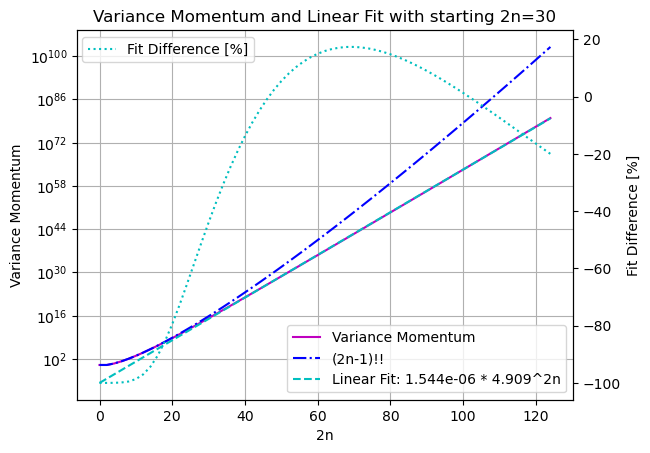
\includegraphics[height=2.5in]{Variance_Momentum.png} 
\captionof{figure}{
The value of variance momentum $\zeta(2n)$ vs the expansion order $2n$ when $\sigma = 5$.
Also included are the uncertainty of the $\zeta(2n)$ due to rounding errors,  $2(n -1)!!$, and the linear fit of the $\zeta(2n)$ value.
}
\label{fig: Variance_Momentum}
\end{figure}



The choice of the bounding factor $\sigma$ needs careful considerations.
If $\sigma = \infty$, $\zeta(2n) = (2n - 1)!!$, which may cause Formula \eqref{eqn: Taylor 1d variance} to diverge in most cases.
When $\sigma$ is limited, Formula \eqref{eqn: variance momentum} becomes Formula \eqref{eqn: momentum factor}:
\begin{itemize}
\item For small $2n$, $\zeta(2n)$ can be approximated by $\zeta(2n) = (2n-1)!!$ according to Formula \eqref{eqn: momentum factor lower}.  

\item For large $2n$, Formula \eqref{eqn: momentum factor} reduces to Formula \eqref{eqn: momentum factor higher}, which shows that $\zeta(2n)$ increases slower than $\sigma^{2n}$ for increasing $2n$.

\end{itemize}
\begin{align}
\label{eqn: momentum factor} 
\zeta(2n) &= 2 N(\sigma) \sigma^{2n} \sum_{j=1}^{\infty} \sigma^{2j-1} \frac{(2n - 1)!!}{(2n-1 + 2j)!!}; \\
\label{eqn: momentum factor lower} 
 &= (2n - 1) \zeta(\sigma, 2n - 2) - 2 N(\sigma) \sigma^{2n - 1}; \\
\label{eqn: momentum factor higher} 
&\sigma^2 \ll 2n:\eqspace \zeta(2n) \simeq 2 N(\sigma) \frac{\sigma^{2n+1}}{2n+1};
\end{align}

The property of $\zeta(2n)$ when $\sigma^2 \ll 2n$ is not sensitive to the underlying uncertainty distribution.  If the normal distribution $N(\tilde{z)}$ in Formula \eqref{eqn: variance momentum} is replaced by a uniform distribution between $[-\sigma, +\sigma]$,  Formula \eqref{eqn: variance momentum UN} is similar to Formula \eqref{eqn: momentum factor higher}:
\begin{align}
\label{eqn: variance momentum UN}
\zeta(2n) &\equiv \int_{-\sigma}^{+\sigma} \frac{1}{2 \sigma} \tilde{z}^{2n} d \tilde{z} = 2 \frac{1}{2 \sigma} \frac{{\sigma}^{2n+1}}{2n + 1}; 
\end{align}

The limited range of $\tilde{x} \in (-\sigma \delta x, +\sigma \delta x)$ causes a bounding leakage $\epsilon$ according to Formula \eqref{eqn: bounding leakage}, in which $\xi(z)$ is the cumulative density function for normal distribution \cite{Probability_Statistics}.
When $\sigma = 5$, $\epsilon = 2 \times 10^{-7}$, which is small enough for most applications.
$\sigma = 5$ is also a golden standard to assert a negative result \cite{Precisions_Physical_Measurements}.
\begin{equation}
\label{eqn: bounding leakage}
\epsilon = 2 - 2 \xi(\frac{1}{2} + \sigma);
\end{equation}

Thus, $\sigma = 5$ in variance arithmetic.  
Figure \ref{fig: Variance_Momentum} shows the value and uncertainties of the corresponding $\zeta(2n)$.
When $2n < 20$, $\zeta(2n)$ can be well approximated by $(2n -1)!!$.  
Formula \eqref{eqn: Taylor 1d variance} and \eqref{eqn: Taylor 1d variance} can be approximated as Formula \eqref{eqn: Taylor 1d variance approx} and \eqref{eqn: Taylor 1d variance approx}, respectively.
\begin{align}
\label{eqn: Taylor 1d variance approx}
\delta^2 f(x) &\simeq (\delta x)^2 (f^{(1)}_x)^2 + (\delta x)^4 \left(f^{(1)}_x f^{(3)}_x + \frac{1}{2} (f^{(2)}_x)^2 \right) \\
  &\eqspace + (\delta x)^6 \left(\frac{1}{4} f^{(1)}_x f^{(5)}_x + \frac{1}{2} f^{(2)}_x f^{(4)}_x + \frac{5}{12} (f^{(3)}_x)^2 \right); \nonumber \\
\label{eqn: Taylor 2d variance approx}
\delta^2 f(x, y)&\simeq (\delta x)^2 (f^{(1,0)}_{(x,y)})^2 + (\delta y)^2 (f^{(0,1)}_{(x,y)})^2 \\
&\eqspace + \left(\delta x)^4 f^{(1,0)}_{(x,y)} (\frac{1}{2} f^{(2,0)}_{(x,y)} + f^{(3,0)}_{(x,y)}\right)
      + (\delta y)^4 \left(\frac{1}{2} f^{(0,2)}_{(x,y)} + f^{(0,1)}_{(x,y)} f^{(0,3)}_{(x,y)}\right) \nonumber \\
&\eqspace + (\delta x)^2 (\delta y)^2 \left((f^{(1,1)}_{(x,y)})^2 + f^{(0,1)}_{(x,y)} f^{(2,1)}_{(x,y)} + f^{(1,0)}_{(x,y)} f^{(1,2)}_{(x,y)}\right); \nonumber
\end{align}


\subsubsection{One-dimensional Examples}

\iffalse

\begin{align*}
e^{x + \tilde{x}} &= e^x \sum_{n=0}^{\infty} \frac{\tilde{x}^n}{n!}
 \simeq e^x \left(1 + \tilde{x} + \frac{1}{2} \tilde{x}^2 + \frac{1}{6} \tilde{x}^3 + \frac{1}{24} \tilde{x}^4 + \frac{1}{120} \tilde{x}^5 + \frac{1}{720} \tilde{x}^6 \right); \\
\overline{e^x} &= e^x \sum_{n=0}^{\infty} (\delta x)^{2n} \zeta(2n) \frac{1}{(2n)!} 
 \simeq e^x \left(1 + \frac{1!!}{2!} (\delta x)^2 + \frac{3!!}{4!} (\delta x)^4 + \frac{5!!}{6!} (\delta x)^6 + \frac{7!!}{8!} (\delta x)^8 \right); \\
P(e^x)^2 &\simeq \frac{\delta^2 e^x}{(e^x)^2} =  \sum_{n=1}^{\infty} (\delta x)^{2n} \left( \zeta(2n) \sum_{j=1}^{2n-1} \frac{1}{j!\;(2n - j)!} 
   	- \sum_{j=1}^{n-1} \frac{\zeta(2j)}{(2j)!}  \frac{\zeta(2n - 2j)}{(2n - 2j)!} \right); \\
 &= (\delta x)^2 + (\frac{7}{4} - \frac{1}{4}) (\delta x)^4 + (\frac{31}{24} - \frac{1}{8}) (\delta x)^6
  + (\frac{127}{192} - \frac{7}{192}) (\delta x)^8 \\
 &= (\delta x)^2 + \frac{3}{2} (\delta x)^4 + \frac{7}{6} (\delta x)^6 + \frac{5}{8} (\delta x)^8
\end{align*}

\begin{align*}
\sin(x + \tilde{x}) - \sin(x) &= \sum_{n=0}^{\infty} \cos(x) (-1)^n \frac{\tilde{x}^{2n+1}}{(2n + 1)!} + \sum_{n=1}^{\infty} \sin(x) (-1)^{n} \frac{\tilde{x}^{2n}}{(2n)!} \\
& \simeq \frac{1}{1!} \cos(x) \tilde{x} - \frac{1}{2!} \sin(x) \tilde{x}^2 - \frac{1}{3!} \cos(x) \tilde{x}^3 + \frac{1}{4!} \sin(x) \tilde{x}^4 + \\
 &\eqspace  \frac{1}{5!} \cos(x) \tilde{x}^5 - \frac{1}{6!} \sin(x) \tilde{x}^6 - \frac{1}{7!} \cos(x) \tilde{x}^7 + \frac{1}{8!} \sin(x) \tilde{x}^8; \\
\overline{\sin(x)} &= \sum_{n=0}^{\infty} \sin(x) (-1)^{n} \frac{\zeta(2n)}{(2n)!} (\delta x)^{2n} \\
 &\simeq  \sin(x) \left(1 - \frac{1!!}{2!} (\delta x)^2 + \frac{3!!}{4!} (\delta x)^4 - \frac{5!!}{6!} (\delta x)^6 + \frac{7!!}{8!} (\delta x)^8 \right); \\
\delta^2 \sin(x) &= \sum_{n=1}^{\infty} (\delta x)^{2n} (-1)^{n - 1}
	\left( \cos(x)^2 \sum_{j=0}^{n-1} \frac{\zeta(2n)}{(2j+1)!(2n-2j-1)!} - \sin(x)^2 \sum_{j=1}^{n-1} \frac{\zeta(2n) - \zeta(2j) \zeta(2n-2j)}{(2j)!(2n-2j)!} \right) \\ 
 &\simeq (\delta x)^2 \cos(x)^2 - (\delta x)^4 \left( \cos(x)^2 - \sin(x)^2 (\frac{3}{4} - \frac{1}{4}) \right) + \\
 &\eqspace (\delta x)^6 \left(\cos(x)^2 \frac{2}{3} - \sin(x)^2 (\frac{5}{8} - \frac{1}{8}) \right) -
    (\delta x)^8 \left(\cos(x)^2 \frac{1}{3} - \sin(x)^2 (\frac{21}{64} - \frac{7}{192}) \right)  \\
 &=  (\delta x)^2 \cos(x)^2 - (\delta x)^4 \left( \cos(x)^2 - \sin(x)^2 \frac{1}{2} \right) + \\
 &\eqspace (\delta x)^6 \left(\cos(x)^2 \frac{2}{3} - \sin(x)^2 \frac{1}{2} \right) - (\delta x)^8 \left(\cos(x)^2 \frac{1}{3} - \sin(x)^2 \frac{7}{24} \right); \\
 &=  (\delta x)^2 \cos(x)^2 - (\delta x)^4 (\cos(x)^2 \frac{3}{2} - \frac{1}{2}) + (\delta x)^6 (\cos(x)^2 \frac{7}{6} - \frac{1}{2})  - (\delta x)^8 (\cos(x)^2 \frac{5}{8} - \frac{7}{24});
\end{align*}

\begin{align*}
& \ln(x + \tilde{x}) - \ln(x) = \ln(1 + \frac{\tilde{x}}{x}) = \sum_{j=1}^{\infty} \frac{(-1)^{j+1}}{j} \frac{\tilde{x}^j}{x^j}; \\
\overline{\ln(x)}  &= \ln(x) -\sum_{n=1}^{+\infty} P(x)^{2n} \frac{\zeta(2n)}{2n}; \\
&\sum_{j=1}^{2n-1} \frac{1}{j} \frac{1}{2n - j} = \frac{1}{2n} \sum_{j=1}^{2n-1} \frac{1}{j} +  \frac{1}{2n - j} = \frac{2}{2n} \sum_{j=1}^{2n-1} \frac{1}{j}
 = \frac{1}{n} \sum_{j=1}^{2n-1} \frac{1}{j}; \\
\delta^2 \ln(x) &= \sum_{n=1}^{+\infty} P(x)^{2n} \left(\sum_{j=1}^{2n-1} \frac{\zeta(2n)}{j (2n-j)}
   - \sum_{j=1}^{n-1} \frac{\zeta(2j)}{2j} \frac{\zeta(2n - 2j)}{2n - 2j} \right) \\
 &= \sum_{n=1}^{+\infty} P(x)^{2n} \left(\frac{\zeta(2n)}{n} \sum_{j=1}^{2n-1} \frac{1}{j} 
     - \sum_{j=1}^{n-1} \frac{\zeta(2j)}{(2j)} \frac{\zeta(2n - 2j)}{(2n - 2j)} \right) \\
 &\simeq P(x)^2 + P(x)^4 (\frac{11}{8} - \frac{1}{4}) + P(x)^6 (\frac{137}{24} - \frac{3}{4}) + P(x)^8 (\frac{1089}{32} - \frac{49}{16}) \\
 &\simeq P(x)^2 + P(x)^4 \frac{9}{8}  + P(x)^6 \frac{119}{24} + P(x)^8 \frac{991}{32};
\end{align*}

\begin{align*}
&(x + \tilde{x})^c = x^c (1 + \frac{\tilde{x}}{x})^c = x^c \sum_{n=1}^{\infty} (\frac{\tilde{x}}{x})^n \begin{pmatrix} c \\ n \end{pmatrix} \\
\frac{(x + \tilde{x})^c}{x^c} &\simeq c (\frac{\tilde{x}}{x}) + \frac{c(c-1)}{2!} (\frac{\tilde{x}}{x})^2
 + \frac{c(c-1)(c-2)}{3!} (\frac{\tilde{x}}{x})^3 + \frac{c(c-1)(c-2)(c-3)}{4!} (\frac{\tilde{x}}{x})^4 + \\
 &\eqspace \frac{c(c-1)(c-2)(c-3)(c-4)}{5!} (\frac{\tilde{x}}{x})^5 + \frac{c(c-1)(c-2)(c-3)(c-4)(c-5)}{6!} (\frac{\tilde{x}}{x})^6; \\
P(x^c)^2 &= \sum_{n=1}^{\infty} P(x)^{2n} \left( \sum_{j=1}^{2n-1} \zeta(2n) \begin{pmatrix} c \\ j \end{pmatrix} \begin{pmatrix} c \\ 2n - j \end{pmatrix}
 - \sum_{j=1}^{n-1} \zeta(2j) \begin{pmatrix} c \\ 2j \end{pmatrix} \zeta(2n - 2j) \begin{pmatrix} c \\ 2n -2 j \end{pmatrix}  \right)\\
 &\simeq c^2 P(x)^2 + \frac{3}{2} c^2 (c-1) (c - \frac{5}{3}) P(x)^4 + \frac{7}{6} c^2 (c-1) (c-2)^2 (c - \frac{16}{7}) P(x)^6;
\end{align*}

\begin{align*}
& (x + \tilde{x})^3 = x^3 + 3 x^2 \tilde{x} + 3 x \tilde{x}^2 + \tilde{x}^3 \\
\overline{x^3} &= x^3 + 3 x (\delta x)^2; \\
\delta^2 x^3 &= 9 x^4  (\delta x)^2 +  (15 x^2 3 - 9 x^2) (\delta x)^4 + 15 (\delta x)^6;
\end{align*}

\fi


Formula \eqref{eqn: exp precision} gives the result variance for $e^x$, which always converge:
\begin{align}
\label{eqn: exp Taylor}
& e^{x + \tilde{x}} = e^x \sum_{n=0}^{\infty} \frac{\tilde{x}^n}{n!}; \\
\overline{e^x} &= e^x + e^x \sum_{n=1}^{\infty} (\delta x)^{2n} \zeta(2n) \frac{1}{(2n)!}; \\
\label{eqn: exp precision}
\widehat{P(e^x)}^2 &= \sum_{n=1}^{\infty} (\delta x)^{2n}  \left( \sum_{j=1}^{2n-1} \frac{\zeta(2n)}{j!\;(2n - j)!} 
 -\sum_{j=1}^{n-1} \frac{\zeta(2j)}{(2j)!} \frac{\zeta(2n - 2j)}{(2n - 2j)!} \right) \\
 &= (\delta x)^2 + \frac{3}{2} (\delta x)^4 + \frac{7}{6} (\delta x)^6 + \frac{5}{8} (\delta x)^8 + o((\delta x)^{10});
\end{align}

Formula \eqref{eqn: log precision} gives the result variance for $\ln(x)$:
\begin{align}
\label{eqn: log Taylor}
& \ln(x + \tilde{x}) - \ln(x) = \ln(1 + \frac{\tilde{x}}{x}) = \sum_{j=1}^{\infty} \frac{(-1)^{j+1}}{j} \frac{\tilde{x}^j}{x^j}; \\
\overline{\ln(x)}  &= \ln(x) -\sum_{n=1}^{+\infty} P(x)^{2n} \frac{\zeta(2n)}{2n}; \\
\label{eqn: log precision}
\delta^2 \ln(x) &= \sum_{n=1}^{+\infty} P(x)^{2n} \left(\sum_{j=1}^{2n-1} \frac{\zeta(2n)}{j (2n-j)}
   - \sum_{j=1}^{n-1} \frac{\zeta(2j)}{2j} \frac{\zeta(2n - 2j)}{2n - 2j} \right) \\
 &= P(x)^2 + P(x)^4 \frac{9}{8}  + P(x)^6 \frac{119}{24} + P(x)^8 \frac{991}{32} + o(P(x)^{10}); 
\end{align}

Formula \eqref{eqn: sin precision} gives the result variance for $\sin(x)$, which converge when $\delta x < 1$:
\begin{align}
\label{eqn: sin Taylor}
& \sin(x + \tilde{x}) = \sum_{n=0}^{\infty} \sin(x) (-1)^{n} \frac{\tilde{x}^{2n}}{(2n)!} + \sum_{n=0}^{\infty} \cos(x) (-1)^n \frac{\tilde{x}^{2n+1}}{(2n + 1)!}; \\
\overline{\sin(x)} &= \sin(x) + \sin(x) \sum_{n=0}^{\infty} (\delta x)^{2n} (-1)^{n} \frac{\zeta(2n)}{(2n)!}; \\
\label{eqn: sin precision}
\delta^2 \sin(x) &= \sum_{n=1}^{\infty} (\delta x)^{2n} (-1)^{n - 1} \\
 & \left( \cos(x)^2 \sum_{j=0}^{n-1} \frac{\zeta(2n)}{(2j+1)!(2n-2j-1)!}
      - \sin(x)^2 \sum_{j=1}^{n-1} \frac{\zeta(2n) - \zeta(2j) \zeta(2n-2j)}{(2j)!(2n-2j)!} \right) \nonumber \\ 
 &=  (\delta x)^2 \cos(x)^2 - (\delta x)^4 (\cos(x)^2 \frac{3}{2} - \frac{1}{2}) + (\delta x)^6 (\cos(x)^2 \frac{7}{6} - \frac{1}{2})  + o((\delta x)^8);
\end{align}

Formula \eqref{eqn: power precision} gives the result variance for $x^c$, in which $\begin{pmatrix} c \\ n \end{pmatrix} = \frac{\prod_{j=0}^{n-1} (c -j)}{n!}$:
\begin{align}
\label{eqn: power Taylor}
&(x + \tilde{x})^c = x^c (1 + \frac{\tilde{x}}{x})^c = x^c + x^c \sum_{n=1}^{\infty} \frac{\tilde{x}^n}{x^n} \begin{pmatrix} c \\ n \end{pmatrix}; \\
\overline{x^c} &= x^c + x^c \sum_{n=1}^{\infty} P(x)^{2n} \zeta(2n) \begin{pmatrix} c \\ 2 n \end{pmatrix}; \\
\label{eqn: power precision}
\widehat{P(x^c)}^2 &= \sum_{n=1}^{\infty} P(x)^{2n} 
 \left( \sum_{j=1}^{2n-1} \zeta(2n) \begin{pmatrix} c \\ j \end{pmatrix} \begin{pmatrix} c \\ 2n - j \end{pmatrix}
 - \sum_{j=1}^{n-1} \zeta(2j) \begin{pmatrix} c \\ 2j \end{pmatrix} \zeta(2n - 2j) \begin{pmatrix} c \\ 2n -2 j \end{pmatrix}  \right)\\
 &= c^2 P(x)^2 + \frac{3}{2} c^2 (c-1) (c - \frac{5}{3}) P(x)^4 + \frac{7}{6} c^2 (c-1) (c-2)^2 (c - \frac{16}{7}) P(x)^6 + o(P(x)^8);
\end{align}
As some special cases for Formula \eqref{eqn: power precision}, Formula \eqref{eqn: square precision} gives the result variance for $x^2$, Formula \eqref{eqn: square root precision} gives the result variance for $\sqrt{x}$, Formula \eqref{eqn: inversion precision} gives the result variance for $1/x$, and Formula \eqref{eqn: inversion square precision} gives the result variance for $1/x^2$: 
\begin{align}
\label{eqn: square precision}
\widehat{P(x^2)}^2 &= 4 P(x)^2 + 2 P(x)^4; \\
\label{eqn: square root precision}
\widehat{P(\sqrt{x})}^2 &= \frac{1}{4} P(x)^2 + \frac{7}{32} P(x)^4 + \frac{75}{128} P(x)^6 + o(P(x)^8); \\
\label{eqn: inversion precision}
\widehat{P(1/x)}^2 &= P(x)^2 + 8 P(x)^4 + 69 P(x)^6 + o(P(x)^8); \\
\label{eqn: inversion square precision}
\widehat{P(1/x^2)}^2 &= 4 P(x)^2 + 66 P(x)^4 + 960 P(x)^6 + o(P(x)^8);
\end{align}


\subsubsection{Convergence and Termination of Taylor Expansion}


If Formula \eqref{eqn: Taylor 1d variance} can be expressed as $\sum_{n=1}^{\infty} \upsilon(2n) \zeta(2n) P(x)^{2n}$, such as Formula \eqref{eqn: log precision} and \eqref{eqn: power precision}, and if $|\upsilon(2n)| \sim \lambda^{2n}$, then Formula \eqref{eqn: Taylor 1d variance} converges if $P(x) < 1/(\lambda \sigma)$.
$\lambda$ depends on $f(x)$, e.g., it is larger for $1/x$ than for $\sqrt{x}$.
The maximal $P(x)$ for Formula \eqref{eqn: Taylor 1d variance} in the $P(x)$-form to converge is defined as the \emph{applicable precision threshold}, which can be estimated as $1/\sigma$ according to Formula \eqref{eqn: momentum factor higher}.

Formula \eqref{eqn: Taylor 1d variance} breaks down near a zero or pole, when the underlying uncertainty distribution deviates significantly from Gaussian, which is the case for $x^c$ at $x=0$, as shown in Figure \ref{fig: Square_Root_Distribution}, \ref{fig: Cubic_Root_Distribution}, \ref{fig: Square_Distribution}, and \ref{fig: Inverse_Square_Distribution}.
Thus, for $(x+a)^c$ in which $a$ is another constant, $P(x) = \delta x / |x - a|$ in Formula \eqref{eqn: power precision}.

The variance formulas using Taylor expansion shows the nature of the calculation, such as $\delta x \rightarrow P(e^x)$, $\delta x \rightarrow \delta \sin(x)$, $P(x) \rightarrow P(x^c)$, and $P(x) \rightarrow \delta \ln(x)$, and the difference speed of variance increases of $x^c$ depending on different $c$.

Both Formula \eqref{eqn: Taylor 1d mean} and \eqref{eqn: Taylor 1d variance} are subject to numerical errors and rounding errors such as from $f^{(j)}_x$, $\zeta(2j)$ and $(\delta x)^{2j}$, so both needs to be calculated using variance arithmetic.
\begin{itemize}
\item  The variance from Formula \eqref{eqn: Taylor 1d mean} can be added to the corresponding result of Formula \eqref{eqn: Taylor 1d variance}.

\item An uncertainty only needs to be correct on order of magnitude, such as with a precision of $1/\sigma=0.2$ or finer.
If the precision of the uncertainty becomes coarser than $1/\sigma$, the result should be invalidated.

\item If within the range of $(x - \sigma \delta x, x + \sigma \delta x)$ an analytic function is monotonic, each term in either Formula \eqref{eqn: Taylor 1d mean} or \eqref{eqn: Taylor 1d variance} should be smaller than its corresponding previous term.
Otherwise, the corresponding sum will diverge, and the result should be invalidated.

\end{itemize}
Variance arithmetic may reject an calculation near a zero or a pole when the variance calculation diverges or becomes uncertain.



\subsection{Dependency Tracing}

\iffalse

\begin{align*}
(f(x) g(x))^{(i)} &= (f(x)^{(1)} g(x) + f(x) g(x)^{(1)})^{(i-1)} \\ 
  &= (f(x)^{(2)} g(x) + 2  f(x)^{(1)} g(x)^{(1)} + f(x) g(x)^{(2)})^{(i-2)} \\
  &= (f(x)^{(3)} g(x) + 3  f(x)^{(2)} g(x)^{(1)} + 3  f(x)^{(1)} g(x)^{(2)} + f(x) g(x)^{(3)})^{(i-3)} \\
  &= \sum_{j=0}^{i} \frac{i!}{j! (i-j)!} f(x)^{(j)} g(x)^{(i-j)}; \\
(f(x)^2 g(x)^2)^{(i)} &=2 \left( (f g) (f g)^{(1)} \right)^{(i-1)} \\
  &= 2 \left( (f g)^{(1)} (f g)^{(1)} + (f g) (f g)^{(2)} \right)^{(i-2)} \\
  &= 2 \left( 3 (f g)^{(1)} (f g)^{(2)} + (f g) (f g)^{(3)} \right)^{(i-3)} \\
  &= 2 \left( 4 (f g)^{(1)} (f g)^{(3)} + 3 (f g)^{(2)} (f g)^{(2)} + (f g) (f g)^{(4)} \right)^{(i-4)}
\end{align*}

\begin{align*}
\delta^2 (c_1 f + c_0) &= c_1^2 \delta^2f; \\
\delta^2 (f + g) &= \overline{(f + g)^2} - \overline{(f + g)}^2 = \overline{f^2} - \overline{f}^2 + 2 \overline{f g} - 2 \overline{f} \overline{g} + \overline{g^2} - \overline{f}^2 \\
 &= \delta^2 f + \delta^2 g + 2 (\overline{fg} - \overline{f}\overline{g}); \\
\overline{f g} &= \sum_{n=0}^{\infty}(\delta x)^{2n} \frac{\zeta(2n)}{(2n)!} (f g)^{(2n)}_x 
  = \sum_{n=0}^{\infty}(\delta x)^{2n} \zeta(2n) \sum_{j=0}^{2n} \frac{f^{(j)}_x}{j!} \frac{g^{(2n - j)}_x}{(2n - j)!};  \\
\overline{f} \overline{g} &= \sum_{n=0}^{\infty}(\delta x)^{2n} \sum_{j=0}^{n} \frac{\zeta(2j) f^{(2j)}_x}{(2j)!} \frac{\zeta(2n - 2j) g^{(2n - 2j)}_x}{(2n - 2j)!};  \\
\delta^2 (f g) &= \overline{f^2 g^2} - \overline{f g}^2; \\
\delta^2 f(g) &= \overline{f(g)^2} - \overline{f(g)}^2;
\end{align*}

When $(f g)^{(n)} = f^{(n)} g^{(n)}$, $\overline{f^n g^n} = \overline{f^n} \overline{g^n}$.
\begin{align*}
\delta^2 (f + g) &= \delta^2 f + \delta^2 g + 2 (\overline{fg} - \overline{f}\overline{g}) =  \delta^2 f + \delta^2 g;  \\
\delta^2 (f g) &= \overline{f^2 g^2} - \overline{f g}^2 = \overline{f^2}\;\overline{g^2} - \overline{f}^2 \overline{g}^2
  = (\delta^2 f + \overline{f}^2)(\delta^2 g + \overline{g}^2) - \overline{f}^2 \overline{g}^2 \\
  &= (\delta^2 f) (\delta^2 g) + \overline{f}^2 (\delta^2 g) + (\delta^2 f) \overline{g}^2; 
\end{align*}

\fi

\begin{align}
\label{eqn: sum variance}
\delta^2 (f + g) &= \delta^2 f + \delta^2 g + 2 (\overline{fg} - \overline{f}\overline{g}); \\
\label{eqn: prod variance}
\delta^2 (f g) &= \overline{f^2 g^2} - \overline{f g}^2; \\
\label{eqn: composite variance}
\delta^2 f(g) &= \overline{f(g)^2} - \overline{f(g)}^2; \\
\label{eqn: linear variance}
\delta^2 (c_1 f + c_0) &= c_1^2 \delta^2f; 
\end{align}

When all the inputs obey the uncorrelated uncertainty assumption, variance arithmetic uses statistics to trace dependency in the intermediate steps.
By convention, variance arithmetic treats different input variables as imprecise values satisfying uncorrelated uncertainty assumption.
For example:
\begin{itemize}
\item Formula \eqref{eqn: sum variance} shows $\delta^2 (f + g)$, whose dependence tracing can be demonstrated by $\delta^2 (f - f) = 0$  and $\delta^2 (f(x) + g(y)) = \delta^2 f + \delta^2 g$, with the latter case corresponding to Formula \eqref{eqn: addition and subtraction}.   

\item Formula \eqref{eqn: prod variance} shows  $\delta^2 (f g)$, whose dependence tracing can be demonstrated by $\delta^2 (f/f) = 0$  and $\delta^2 (f(x) g(y)) = \overline{f}^2 (\delta^2 g) + (\delta^2 f) \overline{g}^2 +  (\delta^2 f) (\delta^2 g)$, with the latter case corresponding to Formula \eqref{eqn: multiplication}.  

\item Formula \eqref{eqn: composite variance} shows  $\delta^2 f(g(x))$, whose dependence tracing can be demonstrated by $\delta^2 (f^{-1}(f)) = \delta^2 x$.  

\item Formula \eqref{eqn: linear variance} shows the variance of linear transformation of a function, which can be applied to Formula \eqref{eqn: sum variance} and \eqref{eqn: prod variance} for more generic dependency tracing.
\end{itemize}
Dependency trading comes with a price: the variance calculation is generally much more complex than the value calculation.


\subsection{Traditional Execution and Dependency Problem}

\iffalse

\begin{align*}
f(g)^{(1)} &= f^{(1)} g^{(1)}; \\
f(g)^{(2)} &= f^{(2)} (g^{(1)})^2 +  f^{(1)} g^{(2)}; \\
f(g)^{(3)} &= f^{(3)} (g^{(1)})^3 + 3 f^{(2)} g^{(1)} g^{(2)} +  f^{(1)} g^{(3)}; \\
f(g)^{(4)} &= f^{(4)} (g^{(1)})^4 + 6 f^{(3)} (g^{(1)})^2 g^{(2)} + 3 f^{(2)} (g^{(2)})^2 + 4 f^{(2)} g^{(1)} g^{(3)} + f^{(1)} g^{(4)}; \\
\delta^2 f(g(x)) &= (\delta x)^2 (f^{(1)}_x g^{(1)}_x)^2 + (\delta x)^4
    ((f^{(1)}_x)^2 (g^{(1)}_x g^{(3)}_x + \frac{1}{2}(g^{(2)}_x)^2) + \frac{1}{2} (f^{(2)}_x)^2 (g^{(1)}_x)^4 \\
  &\eqspace + f^{(1)}_x f^{(2)}_x (g^{(1)}_x)^4 + 4 f^{(1)}_x f^{(2)}_x (g^{(1)}_x)^2 g^{(2)}_x) + o((\delta x)^6); \\
\delta^2 f(x))|_{\delta^2 x = \delta^2 g(x)} &= (\delta x)^2 (f^{(1)}_x g^{(1)}_x)^2 + (\delta x)^4 
    ((f^{(1)}_x)^2 (g^{(1)}_x g^{(3)}_x + \frac{1}{2}(g^{(2)}_x)^2) + \frac{1}{2} (f^{(2)}_x)^2 (g^{(1)}_x)^4 \\
  &\eqspace + f^{(1)}_x f^{(3)}_x (g^{(1)}_x)^4) + o((\delta x)^6) ;
\end{align*}

\begin{align*}
(x + \tilde{x})^2 - (x + \tilde{x}) &= \frac{1}{1!} (2x - 1) \tilde{x} + \frac{1}{2!} 2 \tilde{x}^2 ; \\
\delta^2  (x^{2} - x) &= (2x - 1)^2 (\delta x)^2 + 2 (\delta x)^4; \\
\delta^2 ((x - 1/2)^2 - 1/4) &\longrightarrow (4x^2 - 4x + 1) (\delta x)^2 + 2 (\delta x)^4; \\
\delta^2 (x^{2} - x) &\longrightarrow (4 x^2 + 1) (\delta x)^2 + 2 (\delta x)^4;  \\
\delta^2 (x - 1) x &\longrightarrow (2 x^2 - 2x + 1) (\delta x)^2 + (\delta x)^4 ;
\end{align*}

\fi

\begin{table}
\centering
\begin{tabular}{|l|l|l|} 
\hline 
Formula & Result difference & Wrong independence \\ 
\hline 
\eqref{eqn: interval depend 1} & $0$ & \\
\hline 
\eqref{eqn: interval depend 2} & $4 x (\delta x)^2$ & between $x^2$ and $x$ \\
\hline 
\eqref{eqn: interval depend 3} & $( - 2 x^2 + 2 x) (\delta x)^2 - (\delta x)^4$ & between $x-1$ and $x$ \\
\hline 
\end{tabular}
\captionof{table}{
The dependency problem when applying variance arithmetic without dependency tracing for $x^2 - x$ when the input variance is $(\delta x)^2$.
The correct result variance is $(2 x - 1)^2 (\delta x)^2 + 2 (\delta x)^4$.
}
\label{tbl: dependency example}
\end{table}

Dependency tracing requires final analytic solution to apply Taylor expansion for the result mean and variance, such as using Formula \eqref{eqn: Taylor 1d variance} and \eqref{eqn: Taylor 2d variance}.
It conflicts with traditional numerical executions on analytic functions:
\begin{itemize}

\item
Traditionally, using intermediate variables is a common practice.
But it upsets dependency tracing.

\item 
Traditionally, different analytic expressions of a same function give the same result.
But this is no longer true in variance arithmetic if Taylor expansion is not used.
For example $x^2 - x$ can be calculated equivalently as Formula \eqref{eqn: interval depend 1}, \eqref{eqn: interval depend 2}, and \eqref{eqn: interval depend 3} when applying Formula \eqref{eqn: addition and subtraction}, \eqref{eqn: multiplication}, and \eqref{eqn: square precision} as separated and independent arithmetic operations.
Only Formula \eqref{eqn: interval depend 1} gives the correct result because the input variable $x$ appears only once, while the other two give wrong results for wrong independence assumptions, respectively, as shown in Table \ref{tbl: dependency example}.

\item
Traditionally, conditional executions are used to optimize executions, such as the Gaussian elimination to minimize floating-point rounding errors for matrix inversion \cite{Linear_Algebra}.  
Unless required by mathematics such as for the definition of identity matrix, conditional executions are generally incorrect for dependency tracing, and need to be removed, e.g., Gaussian elimination needs to be replaced by the analytic equations as describe in Section \ref{sec: matrix}.

\item 
Traditionally, approximations on the result values are carried out during executions.
Using variance arithmetic, Formula \eqref{eqn: Taylor 1d variance} shows that the variance converges much slower than that of the value in Taylor expansion, so that the target of approximation should be more on the variance.
Section \ref{sec: matrix} provides an example of first order approximation on calculating matrix determinant.

\item
Traditionally, floating point rounding errors, and numerical errors from library functions work largely in dark.
Variance arithmetic can now illuminates these sources of result uncertainties.
Section \ref{sec: polynomial} and Section \ref{sec: FFT} show that the current traditional floating-point representation is deficient for both traditional Taylor expansion and for variance arithmetic, respectively.

\item
Traditionally, a large calculation may be broken into independent steps, such as calculating $f(g(x))$ as $f(g(x)) = f(y)|_{y = g(x)}$.
But this is no longer true in variance arithmetic due to dependency tracing of $g(x)$ inside $f(g(x))$. 
$\delta^2 f(g(x))$ is calculated as Formula \eqref{eqn: composite variance 1d}, which is different from Formula \eqref{eqn: progressive variance} for $\delta^2 f(x)$ with $\delta^2 x = \delta^2 g(x)$.
The result of Formula \eqref{eqn: progressive variance} depends on the sequence of the composite functions, such as  the difference between Formula \eqref{eqn: square of square root} and \eqref{eqn: square root of square}.
In contrast, the result of Formula \eqref{eqn: composite variance 1d} is not sequence dependent, as shown in Formula \eqref{eqn: square root of square and square of square root}.

\end{itemize}

\begin{align}
\label{eqn: composite variance 1d}
\delta^2 f(g(x)) &\simeq (\delta x)^2 (f^{(1)}_x g^{(1)}_x)^2 \\
  &\eqspace + (\delta x)^4 \left( (f^{(1)}_x)^2 (g^{(1)}_x g^{(3)}_x + \frac{1}{2}(g^{(2)}_x)^2) + \frac{1}{2} (f^{(2)}_x)^2 (g^{(1)}_x)^4 \right) \nonumber \\
  &\eqspace + (\delta x)^4 \left( f^{(1)}_x f^{(2)}_x (g^{(1)}_x)^4 + 4 f^{(1)}_x f^{(2)}_x (g^{(1)}_x)^2 g^{(2)}_x \right) + o((\delta x)^6);  \nonumber\\
\label{eqn: progressive variance}
\delta^2 f(x)|_{\delta^2 x = \delta^2 g(x)} &\simeq (\delta x)^2 (f^{(1)}_x g^{(1)}_x)^2 \\
  &\eqspace + (\delta x)^4 \left( (f^{(1)}_x)^2 (g^{(1)}_x g^{(3)}_x + \frac{1}{2}(g^{(2)}_x)^2) + \frac{1}{2} (f^{(2)}_x)^2 (g^{(1)}_x)^4 \right) \nonumber \\
  &\eqspace + (\delta x)^4 \left( f^{(1)}_x f^{(3)}_x (g^{(1)}_x)^4 \right) + o((\delta x)^6);  \nonumber \\
\label{eqn: square of square root}
\widehat{P(y^2|_{y=\sqrt{x}})}^2 & \simeq P(x)^2 + \frac{9}{2} P(x)^4; \\
\label{eqn: square root of square}
\widehat{P(\sqrt{y}|_{y=x^2})}^2 & \simeq P(x)^2 + \frac{9}{8} P(x)^4; \\
\label{eqn: square root of square and square of square root}
\widehat{P(\sqrt{x}^2)}^2 &= 1 = \widehat{P(\sqrt{x^2})}^2;
\end{align}

Many traditional numerical algorithms are pure numerical, such as numerical equation root finding and Monte Carlo simulation.
Although they cannot be described analytically, their results usually have clear uncertainties, such as the uncertainty for the root.
Variance arithmetic can not apply to them, but can ingest their results.

When the dependency tracing is not applied strictly, variance arithmetic will have dependency problem.
Dependency tracing gets rid of almost all freedoms in the traditional numerical executions, as well as the associated dependence problems.
Because of dependency tracing, variance arithmetic does not suffer from the dependency problem \cite{Interval_Arithmetic} which has plagued interval arithmetic.
All traditional numerical algorithms need to be reexamined or reinvented for variance arithmetic.








\clearpage
\section{Verification of variance arithmetic}
\label{sec: validation}

\subsection{Verification Methods and Standards}

Analytic functions each with precisely known results are used to validate the result uncertainties from variance arithmetic using the following statistical properties: 
\begin{itemize}

\item \emph{value error}: as the difference between the numerical result and the corresponding known precise analytic result.

\item \emph{normalized error}: as the ratio of a value error to the corresponding uncertainty.

\item \emph{error deviation}: as the standard deviation of the normalized errors.

\item \emph{error distribution}: as the histogram of the normalized errors.

\item \emph{uncertainty mean}: as the mean of the result uncertainties.

\item \emph{uncertainty deviation}: as the deviation of the result uncertainties.

\item \emph{error response}: as the relation between the input uncertainties and the result uncertainties.

\item \emph{calculation response}: as the relation between the amount of calculation and the result uncertainties.

\end{itemize}

One goal of calculation involving uncertainty is to precisely account for all input errors from all sources, to achieve \emph{ideal coverage}.
In the case of ideal coverage:
\begin{enumerate}
\item The error deviation is exactly $1$.

\item The central limit theorem converges the result error distribution toward normal distribution.

\item The error response fits the function, such as a linear error response is expected for a linear function.

\item The calculation response fits the function, such as more calculations generally result in larger result uncertainties.

\end{enumerate}
If instead, the input uncertainty is only correct for the input errors on the order of magnitude, the \emph{proper coverage} is achieved when the error deviations are in the range of $[0.1, 10]$.

When the input contains uncertainties whose deviation is not precisely known, such as the numerical errors of library functions, Gaussian or white noises of increasing deviations can be added to the input, until idea coverage is reach.
The needed minimal noise deviation gives a good estimation of the amount of the unspecified input uncertainties.
The existence of ideal coverage is a necessary verification if variance arithmetic correctly tracks the result uncertainty.
The input noise range for the idea coverage defines the ideal application range of input uncertainties.

Gaussian or white noises of specified deviations can also be added to the input to measure the error responses of a function.



\subsection{Types of Uncertainties}

There are five sources of result uncertainty for a calculation \cite{Statistical_Methods}\cite{Numerical_Recipes}:
\begin{itemize}
\item input uncertainties,
\item rounding errors,
\item truncation errors,
\item external errors,
\item modeling errors.
\end{itemize}

The examples in this paper shows that when the input uncertainty precision is $10^{-15}$ or larger, variance arithmetic provides ideal coverage for input uncertainties.

Section \ref{sec: polynomial} shows that variance arithmetic provides proper coverage for floating-point rounding errors.

When the analytic expression is a sum of infinitive diminishing terms, such as a Taylor expression, its numerical implementation needs to truncate the sum to finite terms, possibly causing \emph{truncation errors}.
This process needs to be reevaluated for variance arithmetic. 

The \emph{external errors} are the value errors which are not specified by the input uncertainties, such as the numerical errors in the library math functions.
Section \ref{sec: FFT} studies the effect of $\sin$ and $\tan$ numerical errors, and demonstrates that when the external errors is large enough, neither ideal coverage nor proper coverage can be achieved.
It shows that the library functions need to be recalculated to have corresponding uncertainty attached to each value.

The \emph{modelling errors} arise when an approximate analytic solution is used, or when a real problem is simplified to obtain the solution.  
For example, Section \ref{sec: FFT} demonstrates that the discrete Fourier transformation is only an approximation for the mathematically defined Fourier transformation.  
Conceptually, modelling errors originate from mathematics, so they are outside the domain for variance arithmetic.


\subsection{Types of Calculations to Verify \cite{Prev_Precision_Arithmetic}}

Algorithms of completely different nature with each representative for its category are needed to test the generic applicability of variance arithmetic.  
An algorithm can be categorized by comparing the amount of its input and output data:
\begin{itemize}
\item application
\item transformation
\item generation
\item reduction
\end{itemize}

A \emph{application} algorithm calculate numerical values from an analytic formula. 
Section \ref{sec: polynomial} and \ref{sec: Math Library} show two applications.
In addition to the specified input uncertainty, floating-point rounding errors are hidden input uncertainties.

A \emph{transformation} algorithm has about equal amounts of input and output data.  
The information contained in the data remains about the same after transforming.  
The Discrete Fourier Transformation is a typical transforming algorithm, which contains the same amount of input and output data, and its output data can be transformed back to the input data using essentially the same algorithm.  
For reversible transformations, a unique requirement for variance arithmetic is to introduce the least amount of additional uncertainty after a \emph{round-trip} transformation which is a \emph{forward} followed by a \emph{reverse} transformation.  
The errors after the roundtrip transformation should be delta distributed with $0$ error deviation \footnote{When noises are added to the original input signal, the value errors should be the results minus the overall input data. The previous approaches \cite{Prev_Precision_Arithmetic} used the original input data wrongly.}.
A test of variance arithmetic using FFT algorithms is provided in Section \ref{sec: FFT}.

A \emph{generation} algorithm has much more output data than input data.  
Solving differential equations numerically and generating a numerical table of a specific function are two typical generating algorithms.  
The generating algorithm codes mathematical knowledge into data, so there is an increase of information in the output data.  
Some generating algorithms are theoretical calculations which involve no imprecise input so that all result uncertainty is due to rounding errors.  
Section \ref{sec: recursion} demonstrates such an algorithm, which calculates a table of the sine function using trigonometric relations and two precise input data, $sin(0)=0$ and $sin(\pi/2)=1$.  

A \emph{reduction} algorithm has much less output data than input data such as numerical integration and statistical characterization of a data set.  
Some information of the data is lost while other information is extracted during reducing.  
Conventional wisdom is that a reducing algorithm generally benefits from a larger input data set \cite{Probability_Statistics}.  
A test of statistical characterization through sampling is provided in Section \ref{sec: Math Library}.



\clearpage
\section{Polynomial and Taylor Expansion}
\label{sec: polynomial}

\iffalse

\begin{align*}
(x + \tilde{x})^n &= \sum_{j=0}^{n} \tilde{x}^j x^{n - j}  \begin{pmatrix} n \\ j \end{pmatrix}; \\
f(x + \tilde{x}) &= ( c_0 + c_1 x + c_2 x^2 + c_3 x^3 )  + ( c_1 + c_2 2 x + c_3 3 x^2 ) \tilde{x} +  ( c_2 + c_3 3 x ) \tilde{x}^2 
   + c_3 \tilde{x}^3; \\
f(x + \tilde{x}) &= \sum_{j=0}^{N} c_j (x + \tilde{x})^j 
     = \sum_{j=0}^{N} c_j  \sum_{k=0}^{j} \begin{pmatrix} j \\ k \end{pmatrix} x^{j-k}  \tilde{x}^k
     = \sum_{j=0}^{N} \tilde{x}^{j} \sum_{k=j}^{N} x^{k - j} c_k \begin{pmatrix} k \\ j \end{pmatrix} \\
 & = \sum_{j=0}^{N} \tilde{x}^{j} \sum_{k=0}^{N - j} x^{k} c_{k + j} \begin{pmatrix} j + k \\ j \end{pmatrix} \\   
 &= ( c_0 + c_1 x + c_2 x^2 + c_3 x^3 ) + \tilde{x} (c_1 + c_2 2 x + c_3 3 x^2 ) + \tilde{x}^2 ( c_2 + c_3 3 x ) + \tilde{x}^3 c_3 \\
\overline{f(x)} - f(x) &= \sum_{j=1}^{[N/2]} (\delta x)^{2j} \eta(2j) \sum_{k=0}^{N - 2j} x^{k} c_{k + 2j} \begin{pmatrix} k + 2j \\ 2j \end{pmatrix}
  = (\delta x)^2 ( c_2  + x c_3 3 ); \\
(f(x + \tilde{x}) - f(x))^2 &=
 \sum_{j=1}^{N} \tilde{x}^{j} \sum_{k=0}^{N-j} x^{k} c_{k + j} \begin{pmatrix} j + k \\ j \end{pmatrix} 
 \sum_{m=1}^{N} \tilde{x}^{m} \sum_{n=0}^{N-m} x^{n} c_{n + m} \begin{pmatrix} m + n \\ m \end{pmatrix} \\
    &\eqspace = \sum_{j=1}^{N} \sum_{m=1}^{N} \tilde{x}^{j+m} \sum_{k=0}^{N - j} x^k c_{k+j} \begin{pmatrix} j + k \\ j \end{pmatrix}
		\sum_{n=0}^{N-m} x^n c_{n+m} \begin{pmatrix} n + m \\ n \end{pmatrix}; \\
\delta^2 f(x)  & = \sum_{j=1}^{N} (\delta x)^{2j} \eta(2j) \sum_{m=1}^{j - 1} \sum_{k=0}^{N - 2j + m} x^k c_{k+2j - m} \begin{pmatrix} 2j - m + k \\ 2j - m \end{pmatrix}
		\sum_{n=0}^{N-m} x^n c_{n+m} \begin{pmatrix} n + m \\ n \end{pmatrix} \\
		&\eqspace -  \sum_{j=1}^{[N/2]} (\delta x)^{2j} \sum_{m=1}^{j - 1} \eta(2j - 2m) \eta(2m) 
			\sum_{k=0}^{[N/2] - j + m} x^{2k} c_{2k+2j - 2m} \begin{pmatrix} 2k + 2j - 2m \\ 2j - 2m \end{pmatrix}
			\sum_{n=0}^{[N/2]-m} x^{2n} c_{2n+2m} \begin{pmatrix} 2n + 2m \\ 2n \end{pmatrix};
\end{align*} 

\begin{align*}
c_k &= \begin{pmatrix} k \\ N \end{pmatrix}: \eqspace f(x) = (x + 1)^N; \\
  & c_{n+m} \begin{pmatrix} n \\ n + m \end{pmatrix} = \frac{N!}{(n+m)! (N-n-m)!} \frac{(n+m)!}{n! m!} 
	= \begin{pmatrix} N \\ m \end{pmatrix} \begin{pmatrix} N - m \\ n \end{pmatrix} = \begin{pmatrix} N \\ n \end{pmatrix} \begin{pmatrix} N - n \\ m \end{pmatrix}; \\
\delta^2 f(x)  &= \sum_{j=1}^{N} (\delta x)^{2j} \eta(2j) 
        \sum_{m=1}^{2j - 1} \sum_{k=0}^{N - 2j + m} x^k \begin{pmatrix} N \\ 2j - m \end{pmatrix} \begin{pmatrix} N - (2j - m) \\ k \end{pmatrix}
		\sum_{n=0}^{N-m} x^n \begin{pmatrix} N \\ m \end{pmatrix} \begin{pmatrix} N - m \\ n \end{pmatrix} \\
   &\eqspace -  \sum_{j=1}^{[N/2]} (\delta x)^{2j} \sum_{m=1}^{j - 1} \eta(2j - 2m) \eta(2m) 
		\sum_{k=0}^{[N/2] - j + m} x^{2k} \begin{pmatrix} N \\ 2j - 2m \end{pmatrix} \begin{pmatrix} N - (2j - 2m) \\ 2k \end{pmatrix}
		\sum_{n=0}^{[N/2]-m} x^{2n} \begin{pmatrix} N \\ 2m \end{pmatrix} \begin{pmatrix} N - 2m \\ 2n \end{pmatrix} \\
 &= \sum_{j=1}^{N} (\delta x)^{2j} \eta(2j) 
        \sum_{m=1}^{2j - 1} \begin{pmatrix} N \\ 2j - m \end{pmatrix} (x + 1)^{N - 2j + m} \begin{pmatrix} N \\ m \end{pmatrix} (x + 1)^{N-m} \\
   &\eqspace -  \sum_{j=1}^{[N/2]} (\delta x)^{2j} \sum_{m=1}^{j - 1} \eta(2j - 2m) \eta(2m) 
		(x + 1)^{N - 2j + 2m} \begin{pmatrix} N \\ 2j - 2m \end{pmatrix} (x + 1)^{N - 2m} \begin{pmatrix} N \\ 2m \end{pmatrix} \\
 &= \sum_{j=1}^{N} (\delta x)^{2j} \eta(2j) (x + 1)^{2N - 2j}
        \sum_{m=1}^{2j - 1} \begin{pmatrix} N \\ 2j - m \end{pmatrix} \begin{pmatrix} N \\ m \end{pmatrix} \\
   &\eqspace -  \sum_{j=1}^{[N/2]} (\delta x)^{2j}  (x + 1)^{2N - 2j} \sum_{m=1}^{j - 1} \eta(2j - 2m) \eta(2m) 
		\begin{pmatrix} N \\ 2j - 2m \end{pmatrix} \begin{pmatrix} N \\ 2m \end{pmatrix};
\end{align*}

\begin{align*}
\frac{\delta^2 x^c}{x^{2c}} &= \sum_{n=1}^{\infty} P(x)^{2n} 
 \left( \zeta(2n) \sum_{j=1}^{2n-1} \begin{pmatrix} c \\ j \end{pmatrix} \begin{pmatrix} c \\ 2n - j \end{pmatrix}
 - \sum_{j=1}^{n-1} \zeta(2j) \zeta(2n - 2j) \begin{pmatrix} c \\ 2j \end{pmatrix} \begin{pmatrix} c \\ 2n -2 j \end{pmatrix}  \right);
\end{align*}

\fi

\begin{figure}[p]
\centering
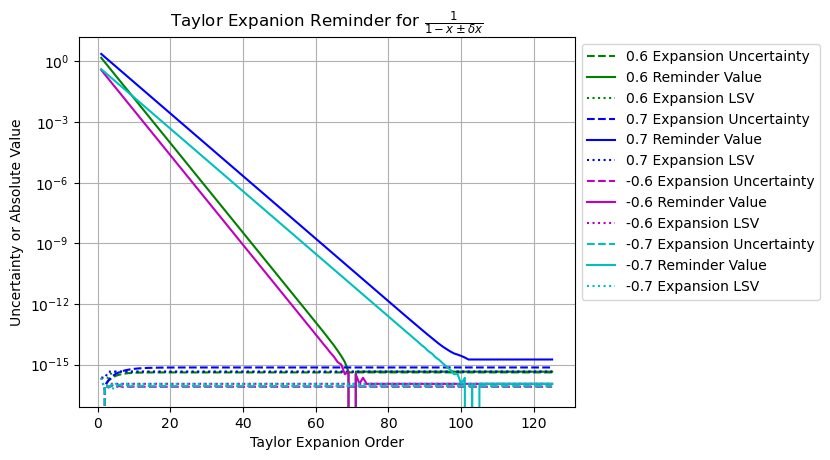
\includegraphics[height=2.5in]{Taylor_Expansion_Uncertainty.png} 
\captionof{figure}{
The absolute reminders and result uncertainties for Taylor expansion of $1/(1-x)$, for different Taylor expansion order $N$ as shown in the x-axis, and different $x$ as shown in the legend.
The y-axis is scaled by the absolute reminder.
In the legend,  
\textit{Absolute Reminder} is the reminder calculated by Formula \eqref{eqn: Taylor expansion reminder}, 
\textit{Uncertainty} is the reminder uncertainty calculated by variance arithmetic,
and \textit{Result LSV} is the least significant value for $1/(1-x)$.
}
\label{fig: Taylor_Expansion_Uncertainty}
\end{figure}

\begin{figure}[p]
\centering
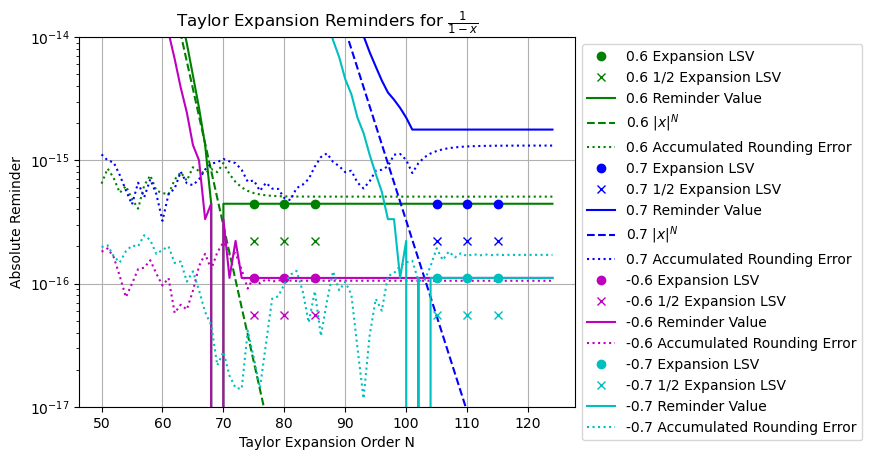
\includegraphics[height=2.5in]{Taylor_Expansion.png} 
\captionof{figure}{
The absolute reminders for Taylor expansion of $1/(1-x)$, for different Taylor expansion order $N$ as shown in the x-axis, and different $x$ as shown in the legend.
The y-axis is scaled by the absolute reminder.
In the legend,  
\textit{Absolute Reminder} is the reminder calculated by Formula \eqref{eqn: Taylor expansion reminder}, 
$x^N$ is the expansion term at Taylor expansion order $N$,
\textit{Result LSV} is the least significant value for $1/(1-x)$,
\textit{Result Half LSV} is half of \textit{Result LSV}, and 
\textit{Accumulated Rounding Error} is the sum of rounding errors of $x^N$.
}
\label{fig: Taylor_Expansion}
\end{figure}


For a polynomial $f(x) \equiv \sum_{j=0}^{N} c_j x^j$, Formula \eqref{eqn: polynomial Taylor} gives the corresponding Taylor expansion:
\begin{equation}
\label{eqn: polynomial Taylor}
f(x + \tilde{x}) = \sum_{j=0}^{N} c_j (x + \tilde{x})^j = \sum_{j=0}^{N} \tilde{x}^{j} \sum_{k=0}^{N-j} x^{k - j} c_{j + k} \begin{pmatrix} j + k \\ j \end{pmatrix};
\end{equation}
When $f(x) = (ax + b)^N$, the result of applying Formula \eqref{eqn: polynomial Taylor} to Formula \eqref{eqn: Taylor 1d variance} is Formula \eqref{eqn: power precision} with $c=N$ and $x = ax + b$. 
Unlike Formula \eqref{eqn: power precision}, applying Formula \eqref{eqn: polynomial Taylor} to Formula \eqref{eqn: Taylor 1d variance} is no longer limited by the applicable precision threshold, because the exponent for power is limited to positive integers.

Formula \eqref{eqn: Taylor inner dependency} shows that Formula \eqref{eqn: Taylor 1d variance} uses Formula \eqref{eqn: sum variance} between any two terms in the Taylor expansion of Formula \eqref{eqn: Taylor 1d}.
It suggests that a Taylor expansion is also a polynomial of Formula \eqref{eqn: polynomial Taylor} with $N \rightarrow \infty$ in variance arithmetic.
\begin{align}
\label{eqn: Taylor inner dependency}
\delta^2 & \left( \frac{f^{(m)}_x \tilde{x}^m}{m!} + \frac{f^{(n)}_x \tilde{x}^n}{n!} \right) = 
    (\delta x)^{2m} (\frac{f^{(m)}_x }{m!})^2 \eta(2m) + (\delta x)^{2n} (\frac{f^{(n)}_x }{n!})^2 \eta(2n) \\
  &+ 2 (\delta x)^{m+n} \left( \frac{f^{(m)}_x f^{(n)}_x}{m! \;n!} \eta(m+n) 	- \frac{f^{(m)}_x}{m!} \eta(m) \;\frac{f^{(n)}_x}{n!}  \eta(n) \right);  \nonumber
\end{align}

A numerical calculation can only calculate limited terms in a Taylor expansion, and the count of terms of the Taylor expansion is needed to approximate a function $f(x)$ is defined as the \emph{Taylor expansion order}.
The needed Taylor expansion order can be obtained by theoretical reminder estimation: If the estimation is less than the least significant value of the current expansion, the Taylor expansion can stop \cite{Numerical_Recipes}.
However, this method does not consider neither floating-point the digital limitation of rounding representation nor floating-point rounding errors, so that it can not guarantee that the result is correct for all significant bits.

Floating-point rounding errors serves as input errors to floating-point calculations, to be a major source of truncation errors.
Taylor expansion for $1/(1-x)$ is used to test the ability of variance arithmetic to predict the effect of floating-point rounding errors.
In Formula \eqref{eqn: Taylor expansion +} and \eqref{eqn: Taylor expansion -}, each $|x|^n$ generates the same rounding error, but the difference in sign means that the same rounding error will have different effects for the summation. 
\begin{align}
\label{eqn: Taylor expansion +}
\frac{1}{1 - |x|} &= 1 + |x| + |x|^2 + |x|^3 + \dots; \\
\label{eqn: Taylor expansion -}
\frac{1}{1 + |x|} &= 1 - |x| + |x|^2 - |x|^3 + \dots; \\
\label{eqn: Taylor expansion reminder}
r(N) & = \left| \lim_{N \rightarrow \infty} \sum_{n = 0}^{N} x^n - \frac{1}{1-x} \right|;
\end{align}
Instead of a reminder estimator, the absolute reminder $r(N)$ is calculated as Formula \eqref{eqn: Taylor expansion reminder} and it is precise.

Figure \ref{fig: Taylor_Expansion_Uncertainty} shows $r(N)$ and the corresponding uncertainties for $x = \pm 0.6, \pm 0.7$.
For $x = \pm 0.6, +0.7$, $r(N)$ reach the least significant values of the precise results, respectively, and the result absolute value errors equal the corresponding result uncertainties, respectively. 
For $x = -0.7$, $r(N)$ does not reach the least significant values of the precise result, leaving the least two significant bits incorrect.
Although the result uncertainty has the correct trend, it does not reach $r(N)$ at the end.

The reason why Formula \eqref{eqn: Taylor 1d variance} does not succeed completely for $x = -0.7$ is due to floating-point rounding errors.
In addition to  the absolute reminder $r(N)$, Figure \ref{fig: Taylor_Expansion} shows the expansion term $x^N$ and the accumulated rounding errors.
\begin{enumerate}
\item When $x^N$ reaches below half of the least significant value of the sum for Formula \eqref{eqn: Taylor expansion +} or \eqref{eqn: Taylor expansion -}, it vanishes so that the corresponding sums stop.

\item When $x^N$ is added to the sum for Formula \eqref{eqn: Taylor expansion +} or \eqref{eqn: Taylor expansion -}, it is digitized by the least significant values $LSV$ of the corresponding sums, to generate rounding error at $n$.
For example, $0.7^{100}=3.23\; 10^{-16}$ is digitized as $4.44\; 10^{-16} = LSV(1/(1 - 0.7))$.
Such digitization is observed to be round to the nearest.

\item The accumulated rounding errors when the sum stop determines the result error.

\item The sign difference in Formula \eqref{eqn: Taylor expansion +} or \eqref{eqn: Taylor expansion -} determines that the accumulated rounding errors for $x = -0.6, -0.7$ are smaller than those for $x = +0.6, +0.7$.

\item When $LSV \ll x^N$, the rounding errors are uniformly distributed, so that the accumulated round errors are close to $0$.
When $x^N$ is close to $LSV$, the accumulated round errors become significant.

\item $x^N$ approaches $LSV$ slower for $x = 0.7$ than that for $x = 0.6$, so the accumulated round errors is larger.

\end{enumerate}
Theoretically, the Taylor convergence range for $\frac{1}{1 - |x|}$ is $|x| < 1$.
To guarantee the Taylor expansion result to be precise, $|x|$ can not be equal or larger than $0.7$.

The reason why Formula \eqref{eqn: Taylor 1d variance} does not succeed completely for $x = -0.7$ is due to the digital limitation of the conventional floating-point representation.
The smallest positive floating-point value is about $5\; 10^{-324}$. 
The least significant value for $0.7$ is about $1\; 10^{-16}$.
At $n=100$, applying Formula \eqref{eqn: polynomial Taylor} to Formula \eqref{eqn: Taylor 1d variance} has $100$ terms in total, but only first $10$ terms can be calculated before $(\delta x)^2$ vanishes.
Thus, variance arithmetic can only provide proper coverage to floating-point rounding errors. 







\clearpage
\section{Matrix Inversion}
\label{sec: matrix}


\subsection{Uncertainty Propagation in Matrix Determinant}

\iffalse

\begin{align*}
|\M| &\equiv \sum_{[p_1\dots p_n]_n} \$ [p_1\dots p_n]_n \prod_{k=1 \dots n} x_{k,p_{k}}; \\
|\M_{<i_1 \dots i_m>_n, [j_1 \dots j_m]_n}| &\equiv \sum_{[p_1 \dots p_n]_n}^{k =1 \dots m:\; p_{i_k}=j_k} \$ [p_1\dots p_n]_n 
	\prod _{k = 1 \dots n }^{i_k \not\in \{i_1 \dots i_m\}} x_{k,p_{k}}; \\
|\M_{<1 \dots n>_n, [j_1 \dots j_n]_n}| &= \$ [j_1\dots j_n]_n; \\
|\M| &= \sum_{{[j_1 \dots j_m]}_n} |\M _{<i_1 \dots i_m>_n, [j_1 \dots j_m]_n}| \prod_{k=1 \dots m} x_{i_k, j_k}; \\
|\M_{<i_1 \dots i_m>_n, [j_1 \dots j_m]_n}| &= \sum_{j \in \{j_1 \dots j_m\}} |\M_{<i_1 \dots i \dots i_m>_n, [j_1 \dots j \dots j_m]_n}| \;x_{i, j};
\end{align*}

\begin{align*}
|\widetilde{M}| &\equiv \sum_{[p_1\dots p_n]_n} \$ [p_1\dots p_n]_n  \prod_{i=1 \dots n} (x_{i,p_i} + \tilde{x}_{i,p_{i}}) \\
	&= \sum_{[p_1 \dots p_{n}]_n} \$[p_1 \dots p_{n}]_n \sum_{m=0 \dots n} \sum_{<i_1 \dots i_m>_n}
		\prod_{i=i_1 \dots i_m} \tilde{x}_{i,p_{i}} \prod_{k = 1 \dots n }^{i_k \not \in \{i_1 \dots i_m\}} x_{k, p_{k}} \\
	&= \sum_{m=0 \dots n} \sum_{<i_1 \dots i_m>_n} \sum_{[j_1 \dots j_{m}]_n} 
		M_{<i_1 \dots i_m>_n, [j_1 \dots j_{m}]_n} \prod_{i=1 \dots m}^{i \in \{i_1 \dots i_m\}} \tilde{x}_{i,p_{i}}
\end{align*}
Examples for $|\widetilde{M}|$:
\begin{align*}
|\tilde{M}| &= x_{0,0} + \tilde{x}_{0,0}; \\
|\tilde{M}| &= \left| \begin{matrix} 
            x_{0,0} + \tilde{x}_{0,0}, x_{0,1} + \tilde{x}_{0,1} \\ 
			x_{1,0} + \tilde{x}_{1,0}, x_{1,1} + \tilde{x}_{1,1} \end{matrix} \right| 
	= (x_{0,0} + \tilde{x}_{0,0})(x_{1,1} + \tilde{x}_{1,1}) - (x_{0,1} + \tilde{x}_{0,1})(x_{1,0} + \tilde{x}_{1,0}) \\
	&= \left| \begin{matrix}  x_{0,0}, x_{0,1} \\  x_{1,0},  x_{1,1} \end{matrix} \right| 
	  + \left| \begin{matrix}  x_{0,0}, \tilde{x}_{0,1} \\  x_{1,0},  \tilde{x}_{1,1} \end{matrix} \right|
	  + \left| \begin{matrix}  \tilde{x}_{0,0}, x_{0,1} \\  \tilde{x}_{1,0},  x_{1,1} \end{matrix} \right|
	  + \left| \begin{matrix}  \tilde{x}_{0,0}, \tilde{x}_{0,1} \\  \tilde{x}_{1,0}, \tilde{x}_{1,1} \end{matrix} \right| \\
|\tilde{M}| &= \left| \begin{matrix} 
            x_{0,0} + \tilde{x}_{0,0}, x_{0,1} + \tilde{x}_{0,1}, x_{0,2} + \tilde{x}_{0,2} \\ 
			x_{1,0} + \tilde{x}_{1,0}, x_{1,1} + \tilde{x}_{1,1}, x_{1,2} + \tilde{x}_{1,2} \\ 
			x_{2,0} + \tilde{x}_{2,0}, x_{2,1} + \tilde{x}_{2,1}, x_{2,2} + \tilde{x}_{2,2} \end{matrix} \right|
	= \left| \begin{matrix} 
	        x_{0,0} + \tilde{x}_{0,0}, x_{0,1} + \tilde{x}_{0,1}, x_{0,2} \\ 
			x_{1,0} + \tilde{x}_{1,0}, x_{1,1} + \tilde{x}_{1,1}, x_{1,2} \\ 
			x_{2,0} + \tilde{x}_{2,0}, x_{2,1} + \tilde{x}_{2,1}, x_{2,2} \end{matrix} \right|
	  + \left| \begin{matrix} x_{0,0} + \tilde{x}_{0,0}, x_{0,1} + \tilde{x}_{0,1}, \tilde{x}_{0,2} \\ 
			x_{1,0} + \tilde{x}_{1,0}, x_{1,1} + \tilde{x}_{1,1}, \tilde{x}_{1,2} \\ 
			x_{2,0} + \tilde{x}_{2,0}, x_{2,1} + \tilde{x}_{2,1}, \tilde{x}_{2,2} \end{matrix} \right| \\
 &= \left| \begin{matrix} 
 		    x_{0,0} + \tilde{x}_{0,0}, x_{0,1}, x_{0,2} \\ 
			x_{1,0} + \tilde{x}_{1,0}, x_{1,1}, x_{1,2} \\ 
			x_{2,0} + \tilde{x}_{2,0}, x_{2,1}, x_{2,2} \end{matrix} \right|
	  + \left| \begin{matrix} 
	        x_{0,0} + \tilde{x}_{0,0}, \tilde{x}_{0,1}, x_{0,2} \\ 
			x_{1,0} + \tilde{x}_{1,0}, \tilde{x}_{1,1}, x_{1,2} \\ 
			x_{2,0} + \tilde{x}_{2,0}, \tilde{x}_{2,1}, x_{2,2} \end{matrix} \right|
	  + \left| \begin{matrix} 
	        x_{0,0} + \tilde{x}_{0,0}, x_{0,1}, \tilde{x}_{0,2}  \\
			x_{1,0} + \tilde{x}_{1,0}, x_{1,1}, \tilde{x}_{1,2} \\ 
			x_{2,0} + \tilde{x}_{2,0}, x_{2,1}, \tilde{x}_{2,2} \end{matrix} \right|
	  + \left| \begin{matrix} 
	        x_{0,0} + \tilde{x}_{0,0}, \tilde{x}_{0,1}, \tilde{x}_{0,2} \\
			x_{1,0} + \tilde{x}_{1,0}, \tilde{x}_{1,1}, \tilde{x}_{1,2} \\ 
			x_{2,0} + \tilde{x}_{2,0}, \tilde{x}_{2,1}, \tilde{x}_{2,2} \end{matrix} \right| \\
 &= \left| \begin{matrix} 
        	x_{0,0}, x_{0,1}, x_{0,2} \\ 
			x_{1,0}, x_{1,1}, x_{1,2} \\ 
			x_{2,0}, x_{2,1}, x_{2,2} \end{matrix} \right|
	  + \left| \begin{matrix} 
	  		\tilde{x}_{0,0}, x_{0,1}, x_{0,2} \\ 
			\tilde{x}_{1,0}, x_{1,1}, x_{1,2} \\ 
			\tilde{x}_{2,0}, x_{2,1}, x_{2,2} \end{matrix} \right|	
	  + \left| \begin{matrix} 
	  		x_{0,0}, \tilde{x}_{0,1}, x_{0,2} \\ 
			x_{1,0}, \tilde{x}_{1,1}, x_{1,2} \\ 
			x_{2,0}, \tilde{x}_{2,1}, x_{2,2} \end{matrix} \right|
      + \left| \begin{matrix} 
      		x_{0,0}, x_{0,1}, \tilde{x}_{0,2}  \\
			x_{1,0}, x_{1,1}, \tilde{x}_{1,2} \\ 
			x_{2,0}, x_{2,1}, \tilde{x}_{2,2} \end{matrix} \right| \\
	  &\eqspace + \left| \begin{matrix} 
	  		\tilde{x}_{0,0}, \tilde{x}_{0,1}, x_{0,2} \\ 
			\tilde{x}_{1,0}, \tilde{x}_{1,1}, x_{1,2} \\ 
			\tilde{x}_{2,0}, \tilde{x}_{2,1}, x_{2,2} \end{matrix} \right|
	  + \left| \begin{matrix} 
	  		\tilde{x}_{0,0}, x_{0,1}, \tilde{x}_{0,2}  \\
			\tilde{x}_{1,0}, x_{1,1}, \tilde{x}_{1,2} \\ 
			\tilde{x}_{2,0}, x_{2,1}, \tilde{x}_{2,2} \end{matrix} \right|
	  + \left| \begin{matrix} 
	  		x_{0,0}, \tilde{x}_{0,1}, \tilde{x}_{0,2} \\
			x_{1,0}, \tilde{x}_{1,1}, \tilde{x}_{1,2} \\ 
			x_{2,0}, \tilde{x}_{2,1}, \tilde{x}_{2,2} \end{matrix} \right|
	  + \left| \begin{matrix} 
	  		\tilde{x}_{0,0}, \tilde{x}_{0,1}, \tilde{x}_{0,2} \\
			\tilde{x}_{1,0}, \tilde{x}_{1,1}, \tilde{x}_{1,2} \\ 
			\tilde{x}_{2,0}, \tilde{x}_{2,1}, \tilde{x}_{2,2} \end{matrix} \right| \\
 &= |\M| + \sum_{i = 0}^{2} \sum_{j = 0}^{2} |\M_{i,j}| \tilde{x}_{i,j} 
 		+ \sum_{<j_1,j_2>} \sum_{[i_1,i_2]} |\M_{[i_1,i_2], <j_1,j_2>}| \tilde{x}_{i_1,j_1} \tilde{x}_{i_2,j_2} \\
 &+ \sum_{<j_1,j_2,j_3>} \sum_{[i_1,i_2,i_3]} \tilde{x}_{i_1,j_1} \tilde{x}_{i_2,j_2} \tilde{x}_{i_3,j_3};
\end{align*}

\begin{align*}
\delta^2 |\M| &= \sum_{m=1}^{n} \sum_{<i_1 \dots i_m>_n} \sum_{[j_1 \dots j_m]_n}
  		|\M _{<i_1 \dots i_m>_n, [j_1 \dots j_m]_n}|^2  \prod_{k=1 \dots n}^{i_k \in \{i_1 \dots i_m\}} (\delta x_{i_k, j_k})^2; \\
\delta^2 |\M_{i,j}| &= \sum_{m=2 \dots n} \sum_{<i_1 \dots i_m>_n}^{i \in \{i_1 \dots i_m\}} \sum_{[j_1 \dots j_m]_n}^{j \in \{j_1 \dots j_m\}}
  	|\M _{<i_1 \dots i_m>_n, [j_1 \dots j_m]_n}|^2  \prod_{k=1 \dots m}^{i_k \in \{i_1 \dots i_m\}, i_k \ne i} (\delta x_{i_k, j_k})^2;
\end{align*}
For each $m$, $\delta^2 |\M|$ has  $\frac{n!}{(n - m)! m!} \frac{n!}{(n - m)!}$ terms, while $\delta^2 |\M_{i,j}|$ has $\frac{(n - 1)!}{(n - m)! (m - 1)!} \frac{(n - 1)!}{(n - m)!}$ terms.  The ratio is $\frac{m^2}{n^2}$.
Thus, the following relation in the previous paper is wrong:
\begin{equation*}
\delta^2 |\M| = \sum_{i=1}^{n} \sum_{j=1}^{n} (\delta x_{i, j})^2 \left(|\M_{i, j}|^2 + \delta^2 |\M_{i,j}| \right);
\end{equation*}
The above relation only holds when $n=2$:
\begin{align*}
|\M| &= \left| \begin{matrix} x_{0,0}, x_{0,1} \\ x_{1,0}, x_{1,1} \end{matrix} \right| = x_{0,0} x_{1,1} - x_{0,1} x_{1,0};  \\
|\tilde{M}| - |\M| &= \tilde{x}_{0,0} x_{1,1} + x_{0,0} \tilde{x}_{1,1} + \tilde{x}_{0,0} \tilde{x}_{1,1}
	 - \tilde{x}_{0,1} x_{1,0} - x_{0,1} \tilde{x}_{1,0} - \tilde{x}_{0,1} \tilde{x}_{1,0}; \\
\delta^2 |\M| &= (\delta x_{0,0})^2 (x_{1,1})^2 + (x_{0,0})^2 (\delta x_{1,1})^2 +  (\delta x_{0,1})^2 (x_{1,0})^2 + (x_{0,1})^2 (\delta x_{1,0})^2 \\
		&+ (\delta x_{0,0})^2 (\delta x_{1,1})^2 + (\delta x_{0,1})^2 (\delta x_{1,0})^2; \\
	&= \delta^2 \left( (x_{0,0} \pm \delta x_{0,0}) (x_{1,1} \pm \delta x_{0,0}) -  (x_{0,1} \pm \delta x_{0,1}) (x_{1,0} \pm \delta x_{0,0}) \right);
\end{align*}
But it does not hold when $n=3$:
\begin{align*}
|\M| &= \left| \begin{matrix} x_{0,0}, x_{0,1}, x_{0,2} \\ x_{1,0}, x_{1,1}, x_{1,2} \\ x_{2,0}, x_{2,1}, x_{2,2} \end{matrix} \right| \\
&= x_{0,0} x_{1,1} x_{2,2} - x_{0,0} x_{1,2} x_{2,1} 
   	+ x_{0,1} x_{1,2} x_{2,0} - x_{0,1} x_{1,0} x_{2,2}
    + x_{0,2} x_{1,0} x_{2,1} -  x_{0,2} x_{1,1} x_{2,0}; \\
\delta^2 |\M| &= (\delta x_{0,0})^2 |\M_{0,0}|^2 + (\delta x_{0,1})^2 |\M_{0,1}|^2 + (\delta x_{0,2})^2 |\M_{0,2}|^2 \\
  &+ (\delta x_{1,0})^2 |\M_{1,0}|^2 + (\delta x_{1,1})^2 |\M_{1,1}|^2 + (\delta x_{1,2})^2 |\M_{1,2}|^2 \\
  &+ (\delta x_{2,0})^2 |\M_{2,0}|^2 + (\delta x_{2,1})^2 |\M_{2,1}|^2 + (\delta x_{2,2})^2 |\M_{2,2}|^2 \\
  &+ (\delta x_{0,0})^2 (\delta x_{1,1})^2 |x_{2,2}|^2 + (\delta x_{0,0})^2 (\delta x_{2,2})^2 |x_{1,1}|^2 + (\delta x_{1,1})^2 (\delta x_{2,2})^2 |x_{0,0}|^2 \\
  &+ (\delta x_{0,0})^2 (\delta x_{1,2})^2 |x_{2,1}|^2 + (\delta x_{0,0})^2 (\delta x_{2,1})^2 |x_{1,2}|^2 + (\delta x_{1,2})^2 (\delta x_{2,1})^2 |x_{0,0}|^2 \\
  &+ (\delta x_{0,1})^2 (\delta x_{1,2})^2 |x_{2,0}|^2 + (\delta x_{0,1})^2 (\delta x_{2,0})^2 |x_{1,2}|^2 + (\delta x_{1,2})^2 (\delta x_{2,0})^2 |x_{0,1}|^2 \\
  &+ (\delta x_{0,1})^2 (\delta x_{1,0})^2 |x_{2,2}|^2 + (\delta x_{0,1})^2 (\delta x_{2,2})^2 |x_{1,0}|^2 + (\delta x_{1,0})^2 (\delta x_{2,2})^2 |x_{0,1}|^2 \\
  &+ (\delta x_{0,2})^2 (\delta x_{1,0})^2 |x_{2,1}|^2 + (\delta x_{0,2})^2 (\delta x_{2,1})^2 |x_{1,0}|^2 + (\delta x_{1,0})^2 (\delta x_{2,1})^2 |x_{0,2}|^2 \\
  &+ (\delta x_{0,2})^2 (\delta x_{1,1})^2 |x_{2,0}|^2 + (\delta x_{0,2})^2 (\delta x_{2,0})^2 |x_{1,1}|^2 + (\delta x_{1,1})^2 (\delta x_{2,0})^2 |x_{0,2}|^2 \\
  &+ (\delta x_{0,0})^2 (\delta x_{1,1})^2 (\delta x_{2,2})^2 + (\delta x_{0,0})^2 (\delta x_{1,2})^2 (\delta x_{2,1})^2 + (\delta x_{0,1})^2 (\delta x_{1,2})^2 (\delta x_{2,0})^2 \\
  &+ (\delta x_{0,1})^2 (\delta x_{1,0})^2 (\delta x_{2,2})^2 + (\delta x_{0,2})^2 (\delta x_{1,0})^2 (\delta x_{2,1})^2 + (\delta x_{0,2})^2 (\delta x_{1,1})^2 (\delta x_{2,0})^2;\\
\end{align*}
\begin{align*}
& (\delta x_{2,2})^2 \delta^2 |\M_{2,2}| = (\delta x_{0,0})^2 (\delta x_{2,2})^2 |x_{1,1}|^2 + (\delta x_{1,1})^2 (\delta x_{2,2})^2 |x_{0,0}|^2 \\
  &+  (\delta x_{0,1})^2 (\delta x_{2,2})^2 |x_{1,0}|^2 + (\delta x_{1,0})^2 (\delta x_{2,2})^2 |x_{0,1}|^2 \\
  &+ (\delta x_{0,0})^2 (\delta x_{1,1})^2 (\delta x_{2,2})^2 + (\delta x_{0,1})^2 (\delta x_{1,0})^2 (\delta x_{2,2})^2; \\
& (\delta x_{2,1})^2 \delta^2 |\M_{2,1}| = (\delta x_{0,0})^2 (\delta x_{2,1})^2 |x_{1,2}|^2 + (\delta x_{1,2})^2 (\delta x_{2,1})^2 |x_{0,0}|^2 \\
  &+  (\delta x_{0,2})^2 (\delta x_{2,1})^2 |x_{1,0}|^2 + (\delta x_{1,0})^2 (\delta x_{2,1})^2 |x_{0,2}|^2 \\
  &+ (\delta x_{0,0})^2 (\delta x_{1,2})^2 (\delta x_{2,1})^2  + (\delta x_{0,2})^2 (\delta x_{1,0})^2 (\delta x_{2,1})^2; \\
& (\delta x_{2,0})^2 \delta^2 |\M_{2,0}| = (\delta x_{0,1})^2 (\delta x_{2,0})^2 |x_{1,2}|^2 + (\delta x_{1,2})^2 (\delta x_{2,0})^2 |x_{0,1}|^2 \\
  &+  (\delta x_{0,2})^2 (\delta x_{2,0})^2 |x_{1,1}|^2 + (\delta x_{1,1})^2 (\delta x_{2,0})^2 |x_{0,2}|^2 \\
  &+ (\delta x_{0,1})^2 (\delta x_{1,2})^2 (\delta x_{2,0})^2 + (\delta x_{0,2})^2 (\delta x_{1,1})^2 (\delta x_{2,0})^2; \\
\delta^2 |\M| & - \sum_{i=0}^{2} \sum_{j=0}^{2} (\delta x_{i,j})^2 |\M_{i,j}| - \sum_{j=0}^{2} (\delta x_{2,j})^2 \delta^2 |\M_{2,j}| \\
  &= (\delta x_{0,0})^2 (\delta x_{1,1})^2 |x_{2,2}|^2 + (\delta x_{0,0})^2 (\delta x_{1,2})^2 |x_{2,1}|^2 \\
  &+ (\delta x_{0,1})^2 (\delta x_{1,2})^2 |x_{2,0}|^2 + (\delta x_{0,1})^2 (\delta x_{1,0})^2 |x_{2,2}|^2 + \\
  &+ (\delta x_{0,2})^2 (\delta x_{1,0})^2 |x_{2,1}|^2 + (\delta x_{0,2})^2 (\delta x_{1,1})^2 |x_{2,0}|^2;
\end{align*}

\begin{align*}
|\M| &= x_{0,0} x_{1,1} x_{2,2} - x_{0,0} x_{1,2} x_{2,1} 
	&+ x_{0,1} x_{1,2} x_{2,0} - x_{0,1} x_{1,0} x_{2,2}
    &+ x_{0,2} x_{1,0} x_{2,1} -  x_{0,2} x_{1,1} x_{2,0}; \\
\end{align*}


Compare $\delta^2 |\M|$ with multiplication:
\begin{align*}
\delta^2 x_1 x_2 &= x_2^2 (\delta x_1)^2 + x_1^2 (\delta x_2)^2 + (\delta x_1)^2 (\delta x_2)^2 \\
\delta^2 x_1 x_2 x_3 &= \left( x_2^2 (\delta x_1)^2 + x_1^2 (\delta x_2)^2 + (\delta x_1)^2 (\delta x_2)^2 \right) x_3^2 + x_1^2 x_2^2 (\delta x_3^2) 
		+ \left( x_2^2 (\delta x_1)^2 + x_1^2 (\delta x_2)^2 + (\delta x_1)^2 (\delta x_2)^2 \right) (\delta x_3^2); \\
	&= (\delta x_1)^2 x_2^2 x_3^2 + x_1^2 (\delta x_2)^2 x_3^2 + x_1^2 x_2^2 (\delta x_3)^2 \\
	&+  x_1^2 (\delta x_2)^2 (\delta x_3)^2 + (\delta x_1)^2 x_2^2 (\delta x_3)^2 + (\delta x_1)^2 (\delta x_2)^2 x_3^2 + (\delta x_1)^2 (\delta x_2)^2 (\delta x_3)^2; \\
\delta^2 \prod_{k=1}^{n} x_k &= \sum_{m=1}^{n} \sum_{<i_1 \dots i_m>_n} \prod_{i \in <i_1 \dots i_m>_n} (\delta x_i)^2 \prod_{j \not \in <i_1 \dots i_m>_n} {x_j}^2;
\end{align*}

\fi

Let vector $[p_1, p_{2} \dots p_n]_n$ denote a permutation of the vector $(1,2\dots n)$ \cite{Linear_Algebra}.  
Let $\$[p_1, p_{2} \dots p_n]_n$ denote the permutation sign of $[p_1, p_{2} \dots p_n]_n$ \cite{Linear_Algebra}. 
Formula \eqref{eqn: determinant} \cite{Linear_Algebra} defines the determinant of a $n$-by-$n$ square matrix $\M$ with the element $x_{i,j}, i,j=1 \dots n$.
The sub-determinant \cite{Linear_Algebra} $M_{i,j}$ at index $(i, j)$ is formed by deleting the row $i$ and column $j$ of $M$, whose determinant is given by 
Formula \eqref{eqn: sub-determinant} \cite{Linear_Algebra}.
Formula \eqref{eqn: determinant sum 1} holds for the arbitrary row index $i$ or the arbitrary column index $j$ \cite{Linear_Algebra}.
\begin{align}
\label{eqn: determinant}
|\M| &\equiv \sum_{[p_1\dots p_n]_n} \$ [p_1\dots p_n]_n \prod_{k=1 \dots n} x_{k,p_{k}}; \\
\label{eqn: sub-determinant}
|\M|_{i,j} &\equiv \sum_{[p_1\dots p_n]_n}^{p_{i} = j} \$ [p_1\dots p_n]_n \prod_{k=1 \dots n}^{k \ne i} x_{k,p_{k}}; \\
\label{eqn: determinant sum 1}
|\M| &=\sum_{j=1 \dots n} |\M_{i,j}| x_{i,j} = \sum_{i=1 \dots n} |\M_{i,j}| x_{i,j};
\end{align}

Assuming $p_1, p_{2} \in \{1\dots n\}$, let $[p_1, p_{2}]_n$ denote the length-2 unordered permutation which satisfies $p_1 \neq p_{2}$, and let $<p_1,p_{2}>_n$ denote the length-2 ordered permutation which satisfies $p_1 < p_{2}$, and let ${<i_1,i_2>}_n$ be an arbitrary ordered permutation \footnote{An ordered permutation is a sorted combination.}. 
Formula \eqref{eqn: determinant sum 1} can be applied to $M_{i,j}$, as:
\begin{align}
&|\M_{<i_1 ,i_{2}>_n, [j_1 ,j_{2}]_n}| \equiv \sum_{[p_1 \dots p_n]_n}^{p_{i_1}=j_1, p_{i_{2}}=j_{2}} 
    \$ [p_1\dots p_n]_n \prod _{k=1 \dots n}^{k \not \in \{i_1, i_2\}} x_{k,p_{k}}; \\
\label{eqn: determinant sum 2}
|\M| &= \sum_{j_1 = 1 \dots n} x_{i_1, j_1} |\M_{i_1, j_1}| = 
\sum_{j_1=1 \dots n} \sum_{j_{2}=1 \dots n}^{ j_{2} \ne j_1} |\M _{<i_1, i_{2}>_n,  [j_1, j_{2}]_n}| x_{i_1, j_1} x_{i_{2}, j_{2}};
\end{align}
The definition of a sub-determinant can be extended to Formula \eqref{eqn: sub-determinant generic}, in which $m =1...n$.  
Formula \eqref{eqn: determinant sum 2} can be generalized as Formula \eqref{eqn: determinant sum}, in which $<i_1 \dots i_m>_n$ is an arbitrary ordered permutation. 
The $(n-m)$-by-$(n-m)$ matrix in $|\M_{<i_1 \dots i_m>_n[j_1 \dots j_m]_n}|$ is obtained by deleting the rows in $\{i_1 \dots i_m\}$ and the columns in $\{j_1 \dots j_m\}$.
This leads to Formula \eqref{eqn: sub-determinant equivalence} \footnote{$\left| |\M| \right|$ in Formula \eqref{eqn: sub-determinant equivalence} means absolute value of determinant.}.
\begin{align}
\label{eqn: sub-determinant generic}
&|\M_{<i_1 \dots i_m>_n, [j_1 \dots j_m]_n}| \equiv \sum_{[p_1 \dots p_n]_n}^{k \in \{i_1 \dots i_m\}: p_k=j_k} \$ [p_1\dots p_n]_n 
	\prod_{k = 1 \dots n }^{k \not \in \{i_1 \dots i_m\}} x_{k,p_{k}}; \\
\label{eqn: determinant sum}
|\M| &= \sum_{{[j_1 \dots j_m]}_n} |\M _{<i_1 \dots i_m>_n, [j_1 \dots j_m]_n}| \prod_{k=1}^{m} x_{i_k, j_k}; \\
\label{eqn: sub-determinant equivalence}
&\left| |\M_{<i_1 \dots i_m>_n, [j_1 \dots j_m]_n}| \right| = \left| |\M_{<i_1 \dots i_m>_n, <j_1 \dots j_m>_n}| \right|;
\end{align}

If all the element of the matrix satisfy the uncorrelated uncertainty assumption, after applying Formula \eqref{eqn: Taylor 2d mean} and \eqref{eqn: Taylor 2d variance}, Formula \eqref{eqn: determinant mean} and \eqref{eqn: determinant variance} are the result mean and variance, respectively.
\begin{align}
\label{eqn: determinant mean}
\overline{|\M|} &= |\M|; \\
\label{eqn: determinant variance}
\delta^2 |\M| &= \sum_{m=1}^{n} \sum_{<i_1 \dots i_m>_n} \sum_{[j_1 \dots j_m]_n}
  	|\M _{<i_1 \dots i_m>_n, <j_1 \dots j_m>_n}|^2 \prod _{k=1 \dots n}^{i_k \in \{i_1 \dots i_m\}} (\delta x_{i_k, j_k})^2; 
\end{align}
Formula \eqref{eqn: determinant mean} and \eqref{eqn: determinant variance} assume that the uncertainties of matrix elements are independent to each other.
In contrast, for the special matrix in Formula \eqref{eqn: special determinant}, after applying Formula \eqref{eqn: Taylor 2d mean} and \eqref{eqn: Taylor 2d variance}, Formula \eqref{eqn: special determinant mean} and \eqref{eqn: special determinant variance} give the result mean and variance, respectively. 
\begin{align}
\label{eqn: special determinant}
|\M| &= \left| \begin{matrix} x, z, y \\ z, y, x \\ y, x, z \end{matrix} \right| = 3 x y z - x^3 - y^3 - z^3; \\
\label{eqn: special determinant mean}
\overline{|\M|} &= |\M| - 3 x (\delta x)^2 - 3 y (\delta y)^2 - 3 z (\delta z)^2; \\
\label{eqn: special determinant variance}
\delta^2 |\M| &= 3 (5 x^4 - 12 x^2 y z + 2 x y^3 + 2 x z^3 + 3 y^2 z^2)(\delta x)^2 \\
 	&+ 3 (5 y^4 - 12 y^2 x z + 2 y x^3 + 2 y z^3 + 3 x^2 z^2)(\delta y)^2 \nonumber \\
 	&+ 3 (5 z^4 - 12 z^2 x y + 2 z x^3 + 2 z y^3 + 3 x^2 y^2)(\delta z)^2 \nonumber \\
 	&+ 9 (z^2 + 2 x y)(\delta x)^2 (\delta y)^2 + 9 (y^2 + x z) (\delta x)^2 (\delta z)^2 + 9 (x^2 +2 y x) (\delta y)^2 (\delta z)^2 \nonumber \\
 	&+ 9 (5 x^2 - 2 y z) (\delta x)^4 + 9 (5 y^2 - 2 x z) (\delta y)^4 + 9 (5z^4 - 2 x y) (\delta z)^4 \nonumber \\
    &+ 15 (\delta x)^6 + 15 (\delta y)^6 + 15 (\delta z)^6 \nonumber;
\end{align}




\subsection{Adjugate Matrix}

\begin{figure}[p]
\centering
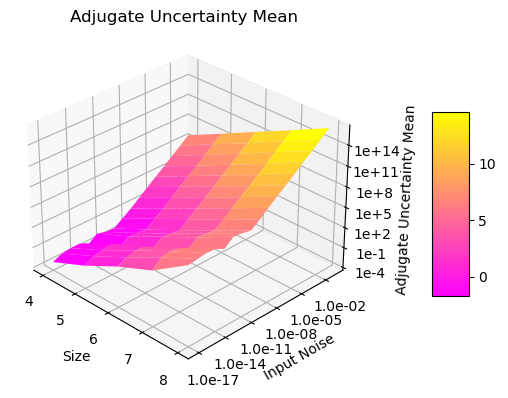
\includegraphics[height=2.5in]{Adjugate_Uncertainty_vs_Size_Noise.png} 
\captionof{figure}{
The result uncertainty means vs. input noise precision and matrix sizefor the difference between $\widehat{\M}^A$ and $\M^A$.
The input noise precision runs from $10^{-17}$ to $10^{-1}$, while the matrix size runs from $4$ to $8$.
}
\label{fig: Adjugate_Uncertainty_vs_Size_Noise}
\end{figure}

\begin{figure}[p]
\centering
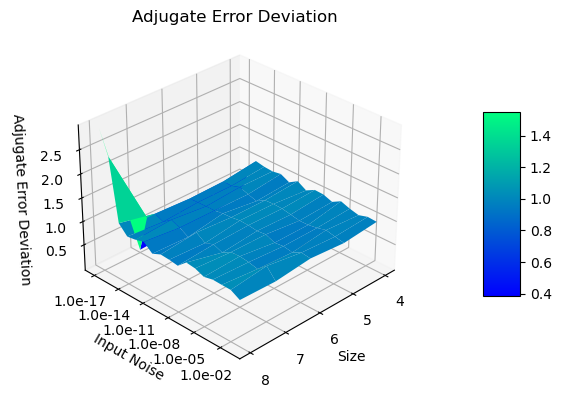
\includegraphics[height=2.5in]{Adjugate_Error_vs_Size_Noise.png} 
\captionof{figure}{
The result error deviations vs. input noise precision and matrix size for the difference between $\widehat{\M}^A$ and $\M^A$.
The input noise precision runs from $10^{-17}$ to $10^{-1}$, while the matrix size runs from $4$ to $8$.
}
\label{fig: Adjugate_Error_vs_Size_Noise}
\end{figure}

\begin{figure}[p]
\centering
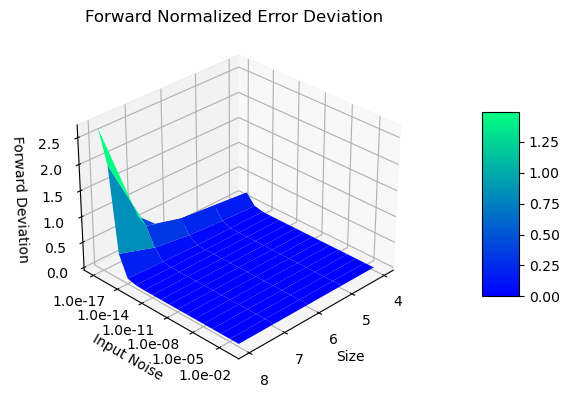
\includegraphics[height=2.5in]{Forward_Error_vs_Size_Noise.png} 
\captionof{figure}{
The result error deviations vs. input noise precision and matrix size for the difference of Formula \eqref{eqn: adjugate matrix}.
The input noise precision runs from $10^{-17}$ to $10^{-1}$, while the matrix size runs from $4$ to $8$.
}
\label{fig: Forward_Error_vs_Size_Noise}
\end{figure}

\begin{figure}[p]
\centering
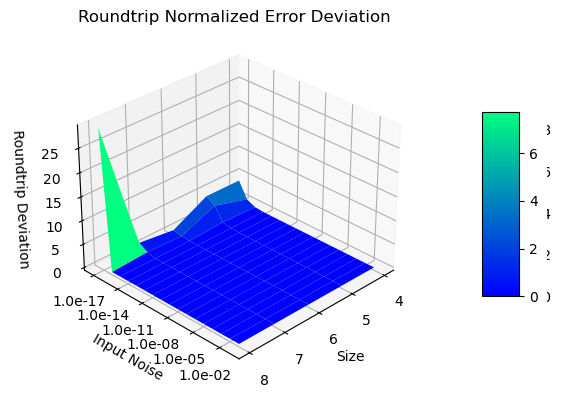
\includegraphics[height=2.5in]{Roundtrip_Error_vs_Size_Noise.png} 
\captionof{figure}{
The result error deviations vs. input noise precision and matrix size for the difference of Formula \eqref{eqn: roundtrip matrix}.
The input noise precision runs from $10^{-17}$ to $10^{-1}$, while the matrix size runs from $4$ to $8$.
}
\label{fig: Roundtrip_Error_vs_Size_Noise}
\end{figure}

\begin{figure}[p]
\centering
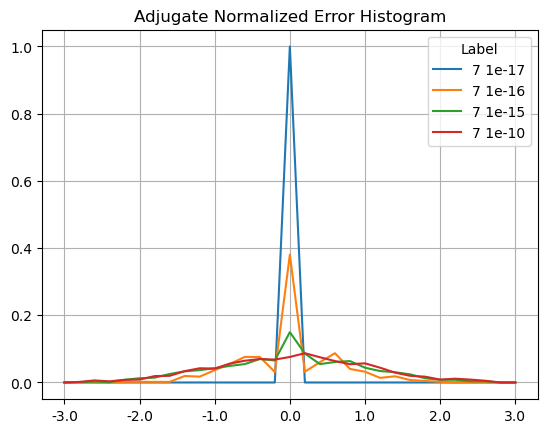
\includegraphics[height=2.5in]{Adjugate_Histogram_Size_7.png} 
\captionof{figure}{
The result histograms for the normalized errors of the adjugate matrix for the same matrix size $7$ and different input noise precision as shown in the legend.
}
\label{fig: Adjugate_Histogram_Size_7}
\end{figure}

\begin{figure}[p]
\centering
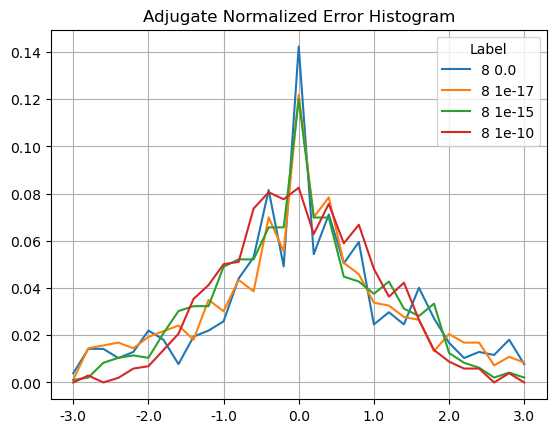
\includegraphics[height=2.5in]{Adjugate_Histogram_Size_8.png} 
\captionof{figure}{
The result histograms for the normalized errors of the adjugate matrix for the same matrix size $8$ and different input noise precision as shown in the legend.
}
\label{fig: Adjugate_Histogram_Size_8}
\end{figure}


The square matrix whose element is $(-1)^{i+j}|\M_{j,i}|$ is defined as the \emph{adjugate matrix} \cite{Linear_Algebra} $\M^A$ to the original square matrix $\M$.
Let $\I$ be the identical matrix for $\M$.
Formula \eqref{eqn: adjugate matrix} and \eqref{eqn: roundtrip matrix} show the relation of $\M^A$ and $\M$ \cite{Linear_Algebra}, which only involve addition, subtraction and multiplication.
\begin{align}
\label{eqn: adjugate matrix}
\M \times \M^A &= \M^A \times \M = |\M| \I; \\
\label{eqn: roundtrip matrix}
|\M| \M^A &=|\M^A| \M;
\end{align}

To test Formula \eqref{eqn: determinant variance}:
\begin{enumerate}
\item A matrix $\M$ is constructed using random integers uniformly distributed in the range of $[-2^8, +2^8]$, which has a distribution deviation of $2^8/\sqrt{3}$.
The integer arithmetic grantees that $|\M|$, $\M^A$, and $|\M^A|$ are precise.

\item Gaussian noises of predefined levels are added to $\M$, to construct $\widehat{\M}$ which contains imprecise values.
variance arithmetic is used to calculate $|\widehat{\M}|$, $\widehat{\M}^A$, and $|\widehat{\M}^A|$.
For example, to construct a $\widehat{\M}$ with $10^{-3}$ input noise precision, the Gaussian noise amplitude is $10^{-3} \times 2^8/\sqrt{3}$.

\item The difference between $|\widehat{\M}|$ and $\M^A$ defines the \emph{Adjugate} Test.
Figure \ref{fig: Adjugate_Uncertainty_vs_Size_Noise} shows that the result uncertainties increase exponentially with both the input noises and the matrix size, while Figure \ref{fig: Adjugate_Error_vs_Size_Noise} shows that the ideal coverage is achieved for the input precision greater than $10^{-16}$.

\item Formula \eqref{eqn: adjugate matrix} defines the \emph{Forward} Test.
Figure \ref{fig: Forward_Error_vs_Size_Noise} shows that Formula \eqref{eqn: adjugate matrix} is strictly observed for the idea coverage.

\item Formula \eqref{eqn: roundtrip  matrix} defines the \emph{Roundtrip} Test.
Figure \ref{fig: Roundtrip_Error_vs_Size_Noise} shows that Formula \eqref{eqn: roundtrip matrix} is strictly observed for the idea coverage.

\end{enumerate}

Figure \ref{fig: Adjugate_Histogram_Size_7} and \ref{fig: Adjugate_Histogram_Size_8} shows that the error values are normal distributed for the input noise precision of  $10^{-10}$, as a typical example of the histograms for ideal coverage.

The existence of ideal coverage validates Formula \eqref{eqn: determinant variance}.


\subsection{Floating Point Rounding Errors}

\begin{table}
\centering
\begin{tabular}{|c|c|c|c|c|} 
\hline 
Error Deviation & \multicolumn{4}{|c|}{Input Noise Precision}  \\ 
\hline 
Matrix Size & $0$ & $10^{-17}$ & $10^{-16}$ & $10^{-15}$ \\ 
\hline 
$4$ & $0$     &       $0$ & $0.68$ & $1.03$ \\
\hline 
$5$ & $0$     & $0.003$ & $0.60$ & $0.96$ \\
\hline 
$6$ & $0$     & $0.006$ & $0.80$ & $1.04$ \\
\hline 
$7$ & $0$     & $0.083$ & $1.05$ & $1.05$ \\
\hline 
$8$ & $4.62$ & $3.91$  & $3.01$ & $1.01$ \\
\hline 
\end{tabular}
\captionof{table}{
The error deviation as a function of matrix size and input noise precision for $\M^A$ in which $\M$ is generated by random integers between $[-2^8, +2^8]$.
The measured error deviations change slightly for different runs.
}
\label{tbl: matrix rounding errors}
\end{table}


The significand of the conventional floating-point representation \cite{Floating_Point_Standard} has $53$-bit resolution, which is equivalent to $10^{-16}$.
Adding noise below this level will not change the value of a conventional floating-point value, so the result uncertainties are caused by the round errors in the floating-point calculations.

Figure \ref{fig: Adjugate_Histogram_Size_7} shows that the histograms of the normalized errors is delta-distributed for the input uncertainty $10^{-17}$, because the adjugate matrix calculation involves about $8 \times 7 = 56$ significand bits for a matrix size $7$.
Such delta distribution also hold when the matrix size is less than $7$, or when the input noise precision is $0$.
When the matrix size is $8$, $8 \times 8 = 64$ significand bits are needed so rounding occurs.
As a result, in Figure \ref{fig: Adjugate_Histogram_Size_8}, the distribution becomes Gaussian with a hint of delta distribution.
Such delta-like distribution persists until the input noise precision reaches $10^{10}$, which is also the transition of the two trends in Figure \ref{fig: Adjugate_Uncertainty_vs_Size_Noise}.

The distribution when the input noise is $0$ is the measured distribution of the conventional floating-point rounding errors.

When the input noise precision increases from $10^{-17}$ to  $10^{-10}$, the distributions become less delta-like and more Gaussian, as shown in both Figure \ref{fig: Adjugate_Histogram_Size_7} and Figure \ref{fig: Adjugate_Histogram_Size_8}. 
The non-ideal behaviors in Figure \ref{fig: Adjugate_Error_vs_Size_Noise}, \ref{fig: Forward_Error_vs_Size_Noise}, and \ref{fig: Roundtrip_Error_vs_Size_Noise} are all attributed to the rounding errors.
Table \ref{tbl: matrix rounding errors} shows that variance arithmetic achieves proper coverage for the calculation rounding errors for adjugate matrix.



\subsection{Matrix Inversion}

\begin{figure}[p]
\centering
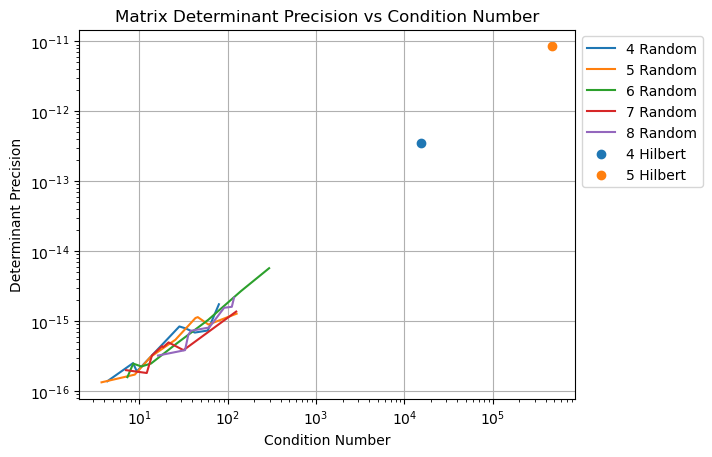
\includegraphics[height=2.5in]{Matrix_Determinant_Prec_vs_Condition.png} 
\captionof{figure}{
The linear correlation between the precision of a matrix determinant to its condition number.
The x-axis shows the condition number, while the y axis shows the precision of the determinant.
The legend shows the size of the matrix, and the type of the matrix as \textit{Random} for randomly generated matrix, and \textit{Hilbert} as the Hilbert matrix.
}
\label{fig: Matrix_Determinant_Prec_vs_Condition}
\end{figure}

A major usage of $|\M|$ and $\M^A$ is to define $\M^{-1}$ in Formula \eqref{eqn: inverse matrix} which satisfies Formula \eqref{eqn: double inverse matrix}.
When $\M$ contains imprecise elements, Formula \eqref{eqn: inverse matrix mean} shows that the direct application of Formula \eqref{eqn: inverse matrix} numerically is wrong, which agrees with the common practice to avoid using Formula \eqref{eqn: inverse matrix} directly \cite{Numerical_Recipes}.
Another reason why not to use Formula \eqref{eqn: inverse matrix} is that according Formula \eqref{eqn: inversion precision}, the denominator uncertainty makes the result precision worse quickly.
\begin{align}
\label{eqn: inverse matrix}
\M^{-1} &\equiv \M^A / |\M|; \\
\label{eqn: double inverse matrix}
(\M^{-1})^{-1} &= \M; \\
\label{eqn: inverse matrix mean}
\overline{\M_{i,j}^{-1}} &\ne |\M_{j,i}| /|\M|;
\end{align}

Traditionally, the effect of uncertainty of  $\M$ to $\M^{-1}$ is quantified by the matrix condition number \cite{Linear_Algebra}.
In Formula \eqref{eqn: inverse matrix}, $\M^{-1}$ is dominated by $1/|\M|$, suggesting that the precision of $\M^{-1}$ is largely determined by the precision of $|\M|$.
Variance arithmetic treats the least significant value of a floating-point value to be imprecise, so it can use Formula \eqref{eqn: special determinant variance} to calculate the determinant variance for a matrix containing floating-point elements, including a randomly generated matrix, or a Hilbert matrix \cite{Linear_Algebra} after it is converted to a floating-point matrix.
Figure \ref{fig: Matrix_Determinant_Prec_vs_Condition} shows that there is a strong linear correlation between the conditional number and the determinant precision of matrices, so that the determinant precision can replace the condition number, which is much more difficult to calculate, and which is somewhat vague for the choices of matrix norms.

In fact, the condition number may not be the best tool to describe the response to input uncertainties of a matrix.
Figure \eqref{eqn: example inverted matrix} shows an example matrix inversion using variance arithmetic representation, in the formation of Formula \eqref{eqn: inverse matrix}.
It clearly shows the overall precision dominance by the value of $72 \pm 87.1$ on the denominator, as well as the the worst element precision $3 \pm 0.5$.
\begin{align}
\label{eqn: example inverted matrix}
\left( \begin{matrix}
	 1 \pm 10^{-1},  &2 \pm 10^{-2},  &3 \pm 10^{-3} \\
	-4 \pm 10^{-4}, &-5 \pm 10^{-5},  &6 \pm 10^{-6} \\
	 7 \pm 10^{-7},  &8 \pm 10^{-8},  &9 \pm 10^{-9}
\end{matrix} \right)^{-1} = \frac{ \left( \begin{matrix}
	&-93 \pm 0.00009,  &6 \pm 0.09,  &27 \pm 0.006 \\
	&78 \pm 0.0009, &-12 \pm 0.9,  &-18 \pm 0.6 \\
	&3 \pm 0.0008,  &6 \pm 0.8,  &3 \pm 0.5
\end{matrix} \right) }{72 \pm 87.1}
\end{align}



\subsection{First Order Approximation}

\begin{figure}[p]
\centering
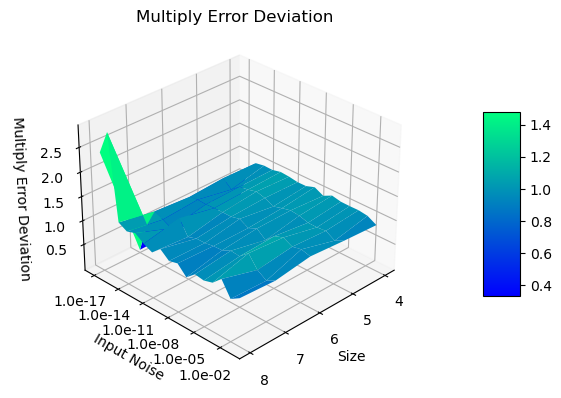
\includegraphics[height=2.5in]{Multiply_Error_vs_Size_Noise.png} 
\captionof{figure}{
The deviation of the first approximation calculation of $|\M|$ vs. input noise precision and matrix size.
}
\label{fig: Multiply_Error_vs_Size_Noise}
\end{figure}

Formula \eqref{eqn: determinant variance approx} gives the first order approximation of Formula \eqref{eqn: determinant variance}, in which $\tilde{x}_{i,j}$ is an imprecise element.
It essentially states that when the input precision is much less than $1$, the determinant $|\M|$ of an imprecise matrix $\M$ can be calculated using Formula \eqref{eqn: determinant} directly.
\begin{equation}
\label{eqn: determinant variance approx}
\delta^2 |\M| \simeq \sum_{i}^{n} \sum_{j}^{n} M_{i,j} (\delta x_{i,j})^2
 = \left( \sum_{[p_1\dots p_n]_n} \$ [p_1\dots p_n]_n \prod_{k=1 \dots n} \tilde{x}_{k,p_{k}} \right)^2 - |\M|^2;
\end{equation}
Figure \ref{fig: Multiply_Error_vs_Size_Noise} contains the result of applying Formula \eqref{eqn: determinant variance approx}.
It is very similar to Figure \ref{fig: Adjugate_Error_vs_Size_Noise}, validating Formula \eqref{eqn: determinant variance approx}.






\clearpage
\section{Moving-Window Linear Regression}
\label{sec: Moving-Window Linear Regression}

\subsection{Moving-Window Linear Regression Algorithm}

\begin{figure}
\centering
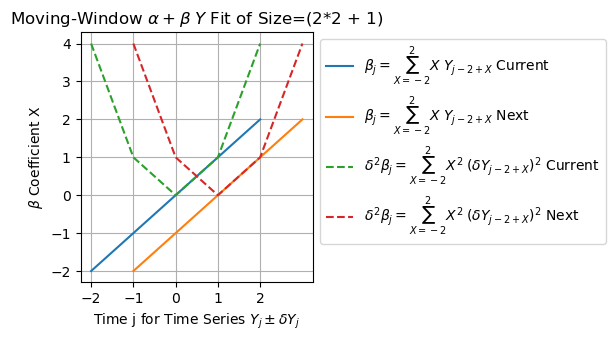
\includegraphics[height=1.75in]{Moving_Linear_Fit_Coeff.png} 
\captionof{figure}{ 
Coefficients of X in Formula \eqref{eqn: time-series linear regression 1} and \eqref{eqn: moving-window linear regression variance 1} at a current and the next position in a time series of the $\alpha + \beta\; Y$ fit. 
It shows that the $\beta_{j+1}$ in Formula \eqref{eqn: time-series linear regression 1} can be calculated progressively from $\beta_j$, as Formula \eqref{eqn: moving-window linear regression 1} and {eqn: moving-window linear regression 0} in order.
It also shows that the $\delta^2 \beta_{j+1}$ in Formula \eqref{eqn: moving-window linear regression variance 1} can not be calculated easily from $\delta^2 \beta_{j}$.
}
\label{fig: Moving_Linear_Fit_Coeff}
\end{figure}

\begin{figure}[p]
\centering
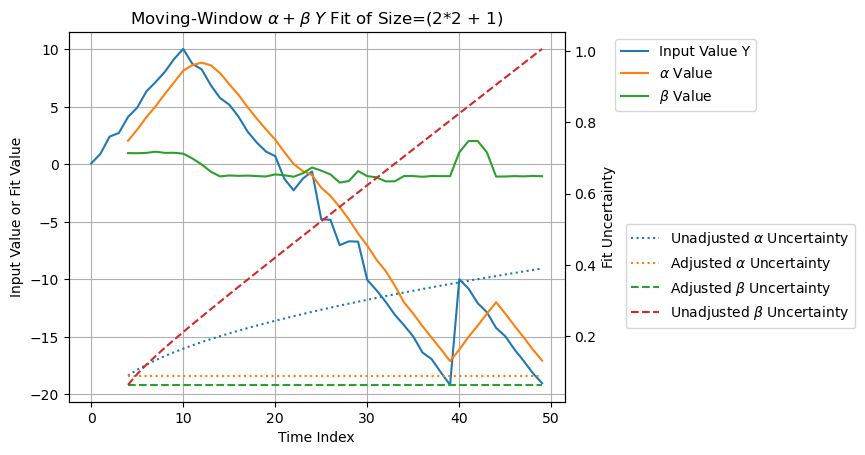
\includegraphics[height=2.5in]{Moving_Linear_Fit_Value.png} 
\captionof{figure}{ 
The input values, fit values, and fit uncertainties of the $\alpha + \beta\; Y$ fit vs time index. 
The x-axis marks the time index.
The y-axis on the left marks the value, while The y-axis on the left marks the uncertainty.
The legend marks different curves.
}
\label{fig: Moving_Linear_Fit_Value}
\end{figure}

\begin{figure}[p]
\centering
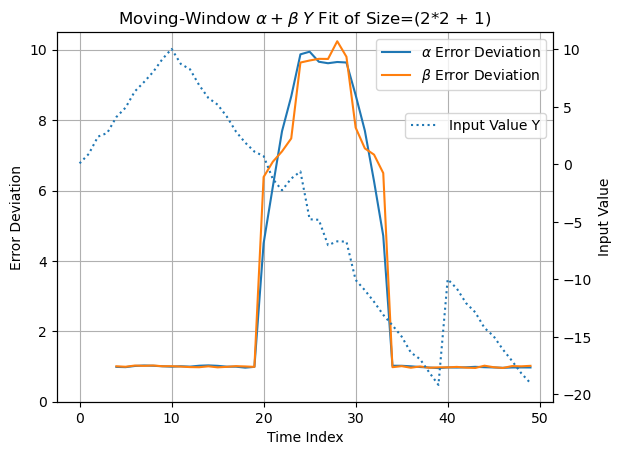
\includegraphics[height=2.5in]{Moving_Linear_Fit_Error.png} 
\captionof{figure}{ 
The error deviations of the $\alpha + \beta\; Y$ fit vs time index. 
The x-axis marks the time index.
The y-axis on the left marks the error deviation.
The legend marks different curves.
}
\label{fig: Moving_Linear_Fit_Error}
\end{figure}



Formula \eqref{eqn: linear regression 0} and \eqref{eqn: linear regression 1} give the result of the least-square line-fit of $Y = \alpha + \beta X$ between two set of data ${Y_j}$ and ${X_j}$, in which $j$ is an integer index to identify $(X, Y)$ pairs in the sets \cite{Numerical_Recipes}.
\begin{align}
\label{eqn: linear regression 0}
\alpha &= \frac{\sum_{j} Y_{j} }{\sum_{j} 1}; \\
\label{eqn: linear regression 1}
\beta &= \frac{\sum_{j} X_{j} Y_{j} \; \sum_{j} 1 - \sum_{j} X_{j} \; \sum_{j} Y_{j}}
    {\sum_{j} X_{j} X_{j} \; \sum_{j} 1 - \sum_{j} X_{j} \; \sum_{j} X_{j} };
\end{align}

In many applications data set ${Y_j}$ is an input data stream collected with fixed rate in time, such as a data stream collected by an ADC (Analogue-to-Digital Converter) \cite{Electronics}.  ${Y_j}$ is called a time-series input, in which $j$ indicates time.  A moving window algorithm \cite{Numerical_Recipes} is performed in a small time-window around each $j$.  For each window of calculation, ${X_j}$ can be chosen to be integers in the range of $[-H, +H]$ in which $H$ is an integer constant specifying window’s half width so that $\sum_{j} X_{j} = 0$, to reduce Formula \eqref{eqn: linear regression 0} and \eqref{eqn: linear regression 1} into Formula \eqref{eqn: time-series linear regression 0} and \eqref{eqn: time-series linear regression 1}, respectively:
\begin{align}
\label{eqn: time-series linear regression 0}
\alpha _{j} &= \alpha \; 2 H = \sum_{X=-H+1}^{H} Y_{j-H+X}; \\
\label{eqn: time-series linear regression 1}
\beta _{j} &= \beta \; \frac{H (H+1)(2H+1)}{3} = \sum_{X=-H}^{H} X Y_{j-H+X}; 
\end{align}
According to Figure \ref{fig: Moving_Linear_Fit_Coeff}, in which $H$ takes an example value of 4, the calculation of $(\alpha _{j}, \beta _{j})$ can be obtained from the previous values of $(\alpha _{j-1}, \beta _{j-1})$, to reduce the calculation of Formula \eqref{eqn: time-series linear regression 0} and \eqref{eqn: time-series linear regression 1} into a progressive moving-window calculation of Formula \eqref{eqn: moving-window linear regression 0} and \eqref{eqn: moving-window linear regression 1}, respectively:
\begin{align}
\label{eqn: moving-window linear regression 0}
\beta _{j} &= \beta _{j-1} - \alpha _{j-1} + H \left(Y_{j-2H-1} + Y_{j} \right); \\
\label{eqn: moving-window linear regression 1}
\alpha_{j} &= \alpha _{j-1} - Y_{j-2H-1} + Y_{j};
\end{align}


\subsection{Variance Adjustment} 

When the time series contain uncertainty, the direct application of Formula \eqref{eqn: moving-window linear regression 0} and \eqref{eqn: moving-window linear regression 1} will result in loss of precision, because both formulas use an same input multiple times and accumulate the variance of the input each time.
In fact, Formula \eqref{eqn: time-series linear regression 1} is better than Formula \eqref{eqn: linear regression 1} because $Y_j$ appears only once in  Formula \eqref{eqn: time-series linear regression 1}.
The value of $\beta_j$ and $\alpha_j$ are given by Formula \eqref{eqn: moving-window linear regression 1} and \eqref{eqn: moving-window linear regression 0}, respectively, while the variance are given by Formula \eqref{eqn: moving-window linear regression variance 0} and \eqref{eqn: moving-window linear regression variance 1}, respectively.
Only Formula \eqref{eqn: moving-window linear regression variance 0} can easily be calculated progressively.
\begin{align}
\label{eqn: moving-window linear regression variance 0}
\delta^2 \alpha_{j} &= \sum_{X=-H+1}^{H} (\delta Y_{j-H+X})^2 = \delta^2 \alpha_{j-1} + (\delta Y_{j})^2 - (\delta Y_{j-2H})^2; \\
\label{eqn: moving-window linear regression variance 1}
\delta^2 \beta_{j} &= \sum_{X=-H+1}^{H} X^2 (\delta Y_{j-H+X})^2;
\end{align}

Figure \ref{fig: Moving_Linear_Fit_Value} shows the input values, fit values, and fit uncertainties of the $\alpha + \beta\; Y$ fit vs time index $j$.
In Figure \ref{fig: Moving_Linear_Fit_Value}, the input signal $Y_j$ is:
\begin{enumerate}
\item An increasing slope for $j = 0 \dots 9$.

\item A decreasing slope for $j = 1 \dots 39$.

\item A sudden jump with an intensity of $+10$ at $j=40$

\item A decreasing slope for $j = 41 \dots 49$.
\end{enumerate}
For each increase of $j$, the increasing rate and the decreasing rate are $+1$ and $-1$, respectively.
The result $\alpha$ and $\beta$ behave correctly with the expected delay in $j$.

Normal noises of $0.2$ intensity are added to the slopes, except Normal noises of $2$ intensity are added to the slope for $j = 10 \dots 19$.
The input uncertainty is always $0.2$.
With the window half size as $H=2$ and the input uncertainty $\delta Y=0.2$, the result uncertainty of $\alpha$ is $\sqrt{\frac{1}{2H+1}} \delta Y$, and the  result uncertainty of $\beta$ is $\sqrt{\frac{3}{H (H+1)(2H+1)}} \delta Y$, both of which are less than the input uncertainty $\delta Y$, due to the averaging effect of the moving window.
Figure \ref{fig: Moving_Linear_Fit_Value} shows that without the variance adjustment, the result uncertainties of $\alpha$ and $\beta$ both increase exponentially with the index time $j$.


\subsection{Unspecified Input Error}

Figure \ref{fig: Moving_Linear_Fit_Error} shows the corresponding error deviation vs index time $j$, which are $1$ except near $10$ for $j = 10 \dots 19$ when the actual noise is $10$-fold of the specified one.
It demonstrates that a larger than $1$ error deviation may probably indicate unspecified additional input errors other than rounding errors, such as the numerical errors from math libraries.




  


\clearpage
\section{Regressive Generation of Sin/Cos}
\label{sec: recursion}

\begin{figure}
\centering
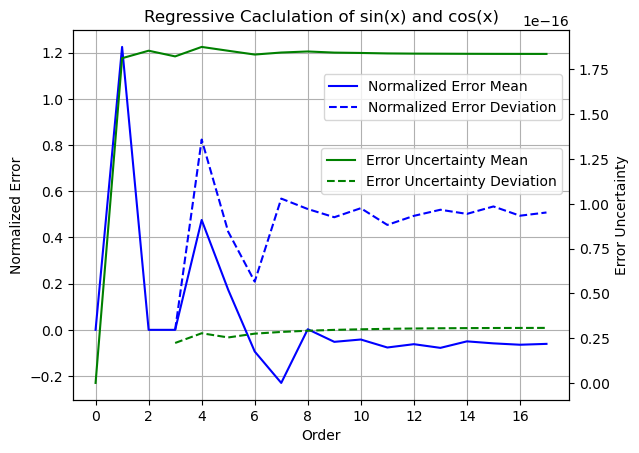
\includegraphics[height=2.5in]{Uncertain_Sin.png}
\captionof{figure}{
The error deviations and uncertainty means for $\sin(x)^2 + \cos(x)^2 - 1, x \in [0, \pi/4]$, for different regression order as shown in the legend.
}
\label{fig: Uncertain_Sin}
\end{figure}

Starting from Formula \eqref{eqn: phase boundary}, Formula \eqref{eqn: phase sin} and Formula \eqref{eqn: phase cos} can be used recursively to calculate the $\sin$ library function.  
\begin{align}
\label{eqn: phase boundary}
& \sin(0) = \cos(\frac{\pi}{2}) = 0; & \sin(\frac{\pi}{2}) = \cos(0) = 1; \\
\label{eqn: phase sin}
& \sin \left(\frac{\alpha + \beta}{2} \right) = \sqrt{\frac{1 - \cos \left(\alpha + \beta \right)}{2}} = & \sqrt{\frac{1 - \cos(\alpha) \cos \left(\beta) + \sin(\alpha \right) \sin(\beta)}{2}}; \\
\label{eqn: phase cos}
& \cos \left(\frac{\alpha + \beta}{2} \right) = \sqrt{\frac{1 + \cos \left(\alpha + \beta \right)}{2}} = & \sqrt{\frac{1 + \cos(\alpha) \cos(\beta) - \sin(\alpha) \sin(\beta)}{2}};
\end{align}
The number of regression is defined as the order.
For each order $n$, $2^n$ $\sin(\frac{\pi}{2} \frac{i}{2^n})$ and $\cos(\frac{\pi}{2} \frac{i}{2^n})$ values are obtained, so that the result is more statistically stable with increasing $n$.

The errors of the generated $\sin(x)$ and $\cos(x)$ are checked by $\sin(x)^2 + \cos(x)^2 - 1$.
The resulted value errors are comparable with but not identical to the value errors using floating-point library $\sin(x)$ and $\cos(x)$.
Figure \ref{fig: Uncertain_Sin} shows that the result uncertainties remain almost a constant of about $1.2 \time 10^{-16}$, which is consist with uniformly distributed least significant values within the least significant bit of the significand.
It also shows that the error deviations is close to $0.5$, which is comparable to the value of $0.535$ for the library $\sin(x)$ and $\cos(x)$ functions.
variance arithmetic is thus effective for this regressive generation algorithm.

Using either Taylor expansion or regressive generation of $\sin(x)$ and $\cos(x)$ are equivalent precision-wise for conventional floating-point calculations.
In contrast, in variance arithmetic, when $x \rightarrow 0$, Formula \eqref{eqn: phase sin} has very coarse precision for Formula \ref{eqn: square root precision}, which result in very coarse precision for $\sin(x)$. 
Thus, variance arithmetic rejects this regressive generation algorithm for $\sin(x)$ and $\cos(x)$.




\clearpage
\section{Math Library Functions}
\label{sec: Math Library}

\begin{figure}[p]
\centering
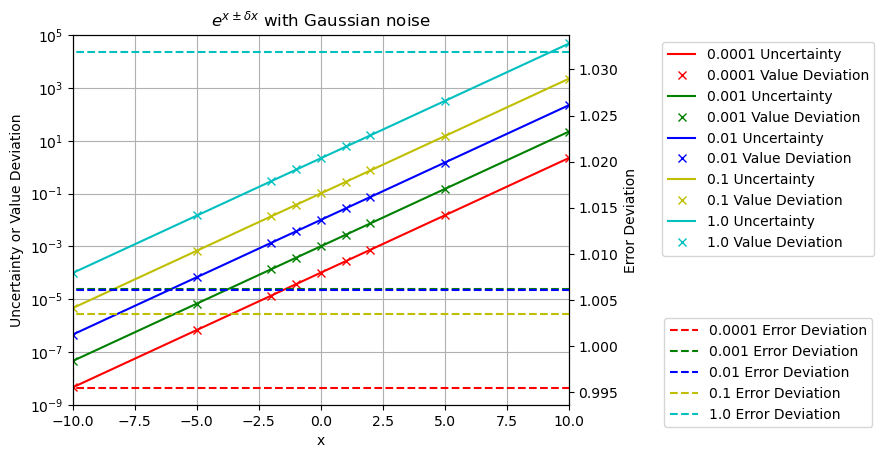
\includegraphics[height=2in]{Exp_Dev.png} 
\captionof{figure}{
The calculated uncertainties vs the measured value deviations and the measured error deviations for $e^{x \pm \delta x}$, for different $\delta x$ as shown in the legend.
The uncertainties and the value deviations are drawn using the logarithmic y scales on the left side, while the error deviations are drawn using the linear y scales on the right side. 
Each color represent a $\delta x$.
Gaussian noises are used to produce the input noise $\delta x$.
}
\label{fig: Exp_Dev}
\end{figure}

\begin{figure}[p]
\centering
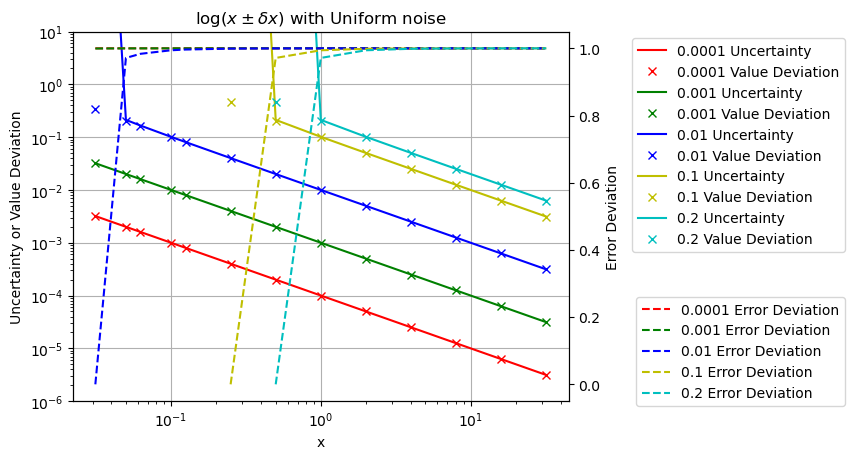
\includegraphics[height=2.5in]{Log_Dev.png} 
\captionof{figure}{
The calculated uncertainties vs the measured value deviations and the measured error deviations for $\log(x \pm \delta x)$, for different $\delta x$ as shown in the legend.
The uncertainties and the value deviations are drawn using the logarithmic y scales on the left side, while the error deviations are drawn using the linear y scales on the right side. 
Each color represent a $\delta x$.
Gaussian noises are used to produce the input noise $\delta x$.
}
\label{fig: Log_Dev}
\end{figure}

\begin{figure}[p]
\centering
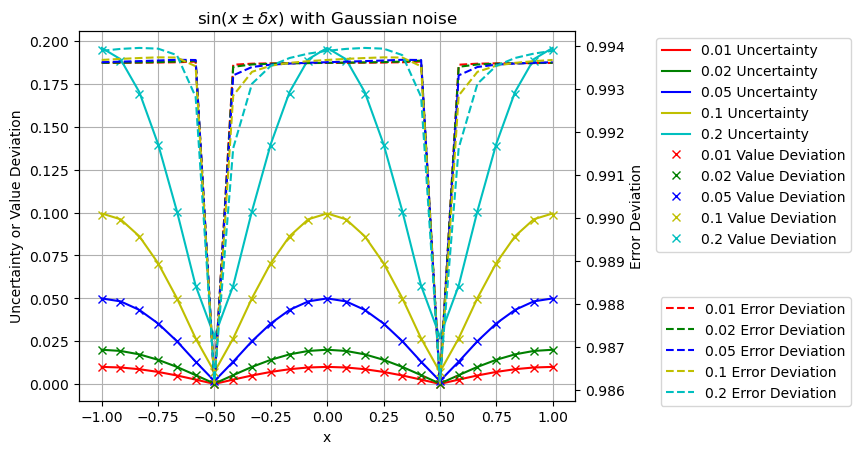
\includegraphics[height=2.5in]{Sin_Dev.png} 
\captionof{figure}{
The calculated uncertainties vs the measured value deviations and the measured error deviations for $\sin(x \pm \delta x)$, for different $\delta x$ as shown in the legend.
The uncertainties and the value deviations are drawn using the logarithmic y scales on the left side, while the error deviations are drawn using the linear y scales on the right side. 
Each color represent a $\delta x$.
Gaussian noises are used to produce the input noise $\delta x$.
}
\label{fig: Sin_Dev}
\end{figure}

\begin{figure}[p]
\centering
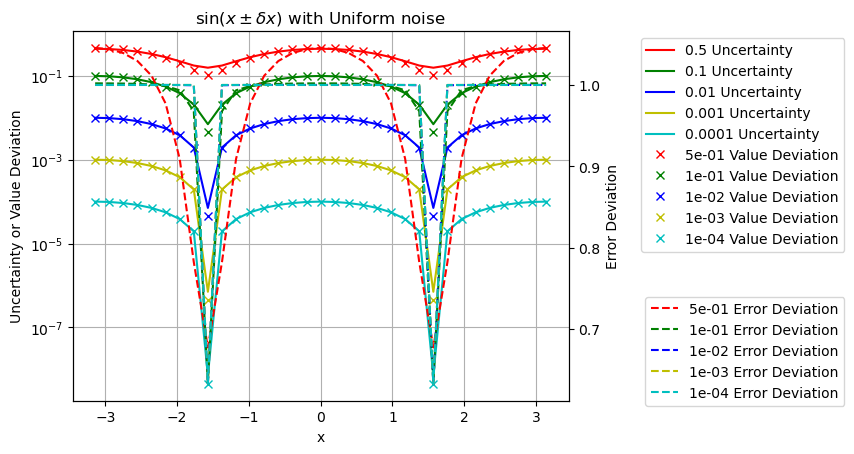
\includegraphics[height=2.5in]{Sin_Dev_Uniform.png} 
\captionof{figure}{
The calculated uncertainties vs the measured value deviations and the measured error deviations for $\sin(x \pm \delta x)$, for different $\delta x$ as shown in the legend.
The uncertainties and the value deviations are drawn using the logarithmic y scales on the left side, while the error deviations are drawn using the linear y scales on the right side. 
Each color represent a $\delta x$.
Uniform noises are used to produce the input noise $\delta x$.
}
\label{fig: Sin_Dev_Uniform}
\end{figure}

\begin{figure}[p]
\centering
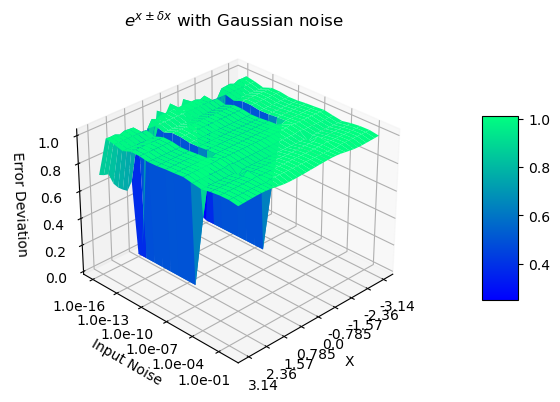
\includegraphics[height=2.5in]{Sin_X_Dev.png} 
\captionof{figure}{
The error deviation for $\sin(x \pm \delta x)$, for $x$ and $\delta$.
The x-axis is $x$ between $-\pi$ and $+\pi$.
The y-axis is $\delta$ between $-10^{-16}$ and $1$.
The z-axis is the error deviation. 
Gaussian noises are used to produce the input noise $\delta x$.
}
\label{fig: Sin_X_Dev}
\end{figure}

\begin{figure}[p]
\centering
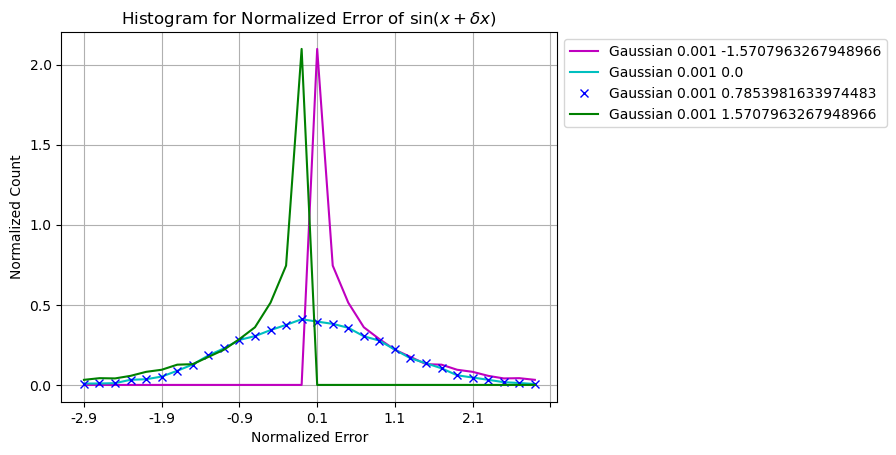
\includegraphics[height=2.5in]{Sin_Histo.png} 
\captionof{figure}{
The histogram of the error deviation for $\sin(x \pm \delta x)$, for $x=-\pi/2, -\pi/4, 0, +\pi/4, +\pi/2$ and $\delta x = 10^{-1}, 10^{-16}$ as shown in the legend.
The y-axis is the normalized count. 
Each color represents a different $x$, while each line pattern represents a different $\delta x$.
Uniform noises are used to produce the input noise $\delta x$.
}
\label{fig: Sin_Histo}
\end{figure}

\begin{figure}[p]
\centering
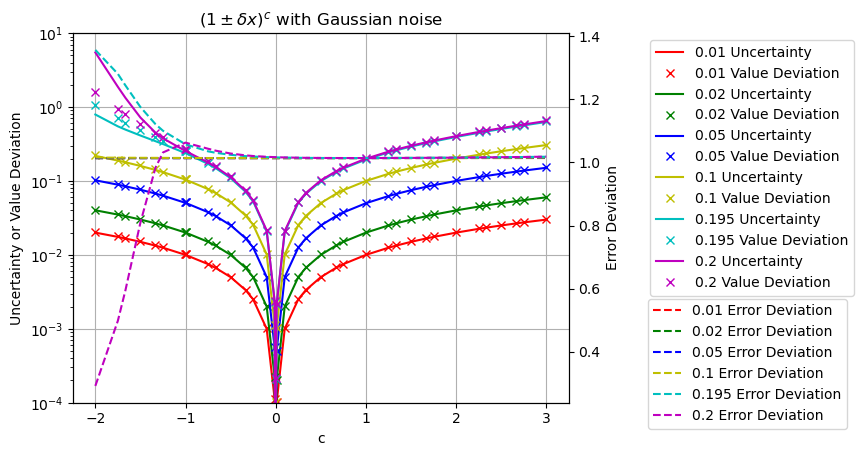
\includegraphics[height=2.5in]{Pow_Dev.png} 
\captionof{figure}{
The calculated uncertainties vs the measured value deviations and the measured error deviations for $(1 \pm \delta x)^c$, for different $\delta x$ as shown in the legend.
The uncertainties and the value deviations are drawn using the logarithmic y scales on the left side, while the error deviations are drawn using the linear y scales on the right side. 
Each color represent a $\delta x$.
}
\label{fig: Pow_Dev}
\end{figure}

\begin{figure}[p]
\centering
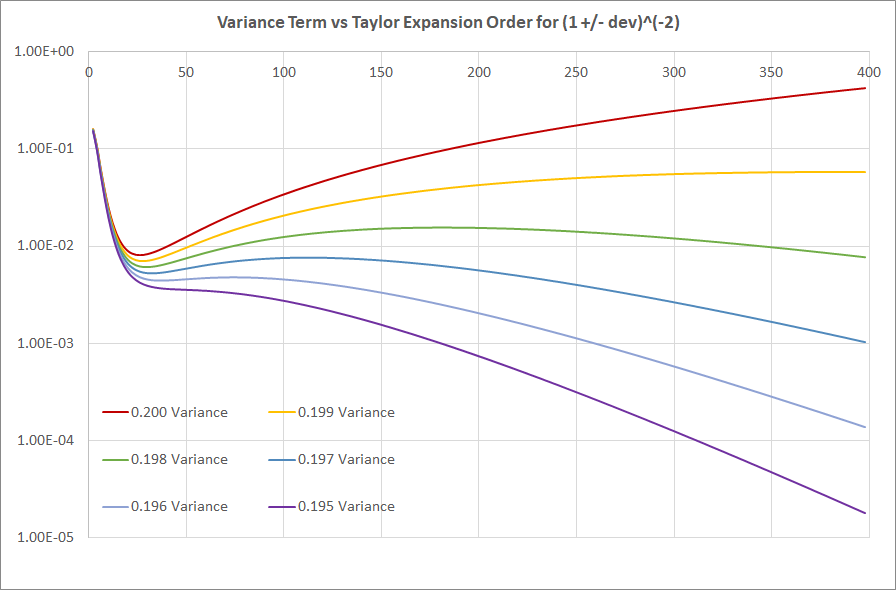
\includegraphics[height=2.5in]{Pow_Converge.png} 
\captionof{figure}{
The individual variance term of $(1 \pm \delta x)^c$ vs the different Taylor expansion order $2n$, for different $c$ and $\delta x$ as shown in the legend. 
The $x$-axis is Taylor expansion order $2n$ from 1 to 400 in Formula \eqref{eqn: Taylor 1d variance}.
The $y$-axis is the contribution to $(1 \pm \delta x)^c$ at each Taylor expansion order $2n$ according to Formula \eqref{eqn: power precision}.
It shows that $(1 \pm 0.2)^{-2}$ and $(1 \pm 0.2)^{-1.5}$ clearly diverge, $(1 \pm 0.2)^{-1}$ seems diverges, and other cases clearly converge.
}
\label{fig: Pow_Converge}
\end{figure}

\begin{figure}[p]
\centering
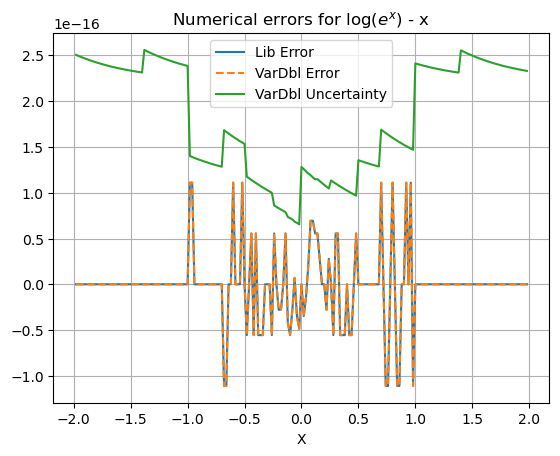
\includegraphics[height=2.5in]{ExpLog_Error.png} 
\captionof{figure}{
The values and uncertainties of $\log(e^x) - x$ vs $x$, as \textit{VarDbl Error} and \textit{VarDbl Uncertainty} in the legend.
The result of the same calculation using conventional floating-point library functions is shown as \textit{Lib Error} in the legend.
}
\label{fig: ExpLog_Error}
\end{figure}

\begin{figure}[p]
\centering
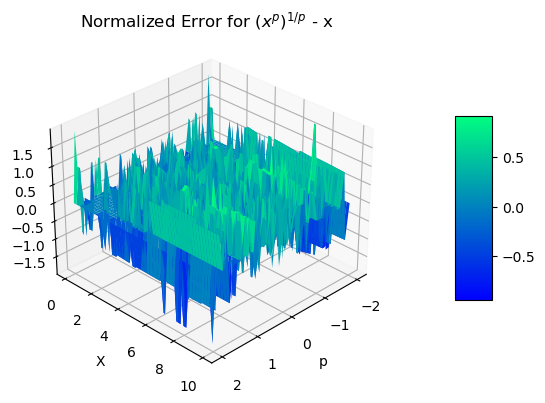
\includegraphics[height=2.5in]{Power_Error.png} 
\captionof{figure}{
The normalized errors of $(x^p)^{\frac{1}{p}} - x$ vs $x$ and $p$.
}
\label{fig: Power_Error}
\end{figure}


Formula \eqref{eqn: exp precision}, \eqref{eqn: log precision}, \eqref{eqn: sin precision}, and \eqref{eqn: power precision} are tested by the corresponding math library functions \textit{exp}, \textit{log}, \textit{sin}, and \textit{pow}, respectively.

At each point $x$ for an input uncertainty $\delta x$, the result uncertainty is calculated by variance arithmetic.
The corresponding value deviation is obtained by:
\begin{enumerate}

\item Take $10000$ samples from either Gaussian noise or uniform distribution with $\delta x$ as the deviation, and construct $\tilde{x}$ which is $x$ plus the sampled noise.  

\item For each $\tilde{x}$, use the corresponding library function to calculate the value error as the difference between using $\tilde{x}$ and using $x$ as the input.

\item The value error is divided by the result uncertainty, as the normalized error.

\item The standard deviation of the $10000$ normalized errors is the error deviation.

\item In addition, for each of these tests, all value errors follow a same underlying distribution.
The deviation of the value errors is defined as the \emph{value deviation}, which the uncertainty should match.

\end{enumerate}

\subsection{Exponential}

Figure \ref{fig: Exp_Dev} shows that the calculated uncertainties using Formula \eqref{eqn: exp precision} agree very well with the measured value deviations for $e^{x + \delta x}$.
As a result, the error deviations are very close to $1$, even both the uncertainties and the value error deviations increase exponentially with $x$ and $\delta x$.
Such strong tracking power holds for all $x$ of $e^{x + \delta x}$. 

\subsection{Logarithm}

Figure \ref{fig: Log_Dev} shows that the calculated uncertainties using Formula \eqref{eqn: log precision} agree very well with the measured value deviations for $\log(x + \delta x)$, so that the result error deviations are very close to $1$, until the uncertainties suddenly diverge when the input precision is coarser than $1/5$ which is the estimated application precision threshold.
After the result uncertainties diverge, the corresponding value deviations still continue on the same trends until the input data to the $\log$ function start to have negative values whenthe input noises are uniformly distributed.
If Gaussian noises are used instead, the cutoffs for both value errors and error deviations are strictly at $1/5$.
The result probability density function for $\log(x)$ has a pole at $x=0$.

Such divergences of the result uncertainties are expected when the input precision is coarser than the estimated applicable precision threshold of $1/\sigma$, in which $\sigma=5$ is the bonding factor of variance arithmetic.
If $\sigma$ is reduced from $5$ to $4$, the measured applicable precision thresholds increase from $1/5$ to $1/4$, allowing more result uncertainties to be valid.
The reduction of $\sigma$ increases the bounding leakage $\epsilon$ from $5.7 \times 10^{-7}$ to $6.3 \times 10^{-5}$ according to Formula \eqref{eqn: bounding leakage}.
A large leakage $\epsilon$ raises the logic questions on the validity of the result, because the leakage may mean $x \leq 0$ for $\log(x)$ in this case.
In an extreme approach, in another variance arithmetic representation:
\begin{enumerate}

\item Each imprecise value carries its own $\sigma$ or $\epsilon$ to indicate the statistical significance of its value to its uncertainty.

\item The result $\sigma$ or $\epsilon$ involving two imprecise values can be found statistically.

\item The result of an analytic function always converges but at the expense of $\epsilon$, such that  when $x \rightarrow 0$, $\epsilon \rightarrow 1$ for $\log(x + \delta x)$. 

\item A calculation may branch based on the probability $\epsilon$.

\end{enumerate}
For the discussion simplicity, the cases of the bounding factor $\sigma$ other than constant $5$ are avoided in this paper.




\subsection{Sine}

Figure \ref{fig: Sin_Dev} shows that the calculated uncertainties using Formula \eqref{eqn: sin precision} agree very well with the measured value deviations for $\sin(x + \delta x)$.
Figure \ref{fig: Sin_Dev} also shows that $\delta^2 \sin(x)$ has the same periodicity as $\sin(x)$:
\begin{itemize}
\item When $x=0$, $\sin(x) \simeq x$, so that $\delta^2 \sin(x) \simeq (\delta x)^2$.
\item When $x=\pi/2$, $\sin(x) \simeq 1$, so that $\delta^2 \sin(x) \simeq 0$.
\end{itemize}

In Figure \ref{fig: Sin_Dev}, Gaussian noises are used, while in Figure \ref{fig: Sin_Dev_Uniform}, ideal white noises are added for then given sample size of $10000$.
The difference of Figure \ref{fig: Sin_Dev} and \ref{fig: Sin_Dev_Uniform} shows that the Gaussian noise is more desirable, because of its tail effect, e.g., the error deviation is much closer to $1$ for $\sin(\pm \pi/2 + \delta x)$.
So only Gaussian noises will be used for other analysis by default.

Figure \ref{fig: Sin_X_Dev} shows that the error deviation for $\sin(x + \delta x)$ is $1$ except when $x=\pm \pi/4$ and $\delta x < 10^{-12}$, at where the probability density function has a zero.
Figure \ref{fig: Sin_Histo} shows the histogram of the error deviation for $\sin(x + \delta x)$ when Gaussian noises are used to produce the input noise $\delta x$:
\begin{itemize}
\item When $\delta x=10^{-16}$, the noise is comparable to the numerical calculation error of $\sin(x)$.
The histogram is highly structured, with peaks near $0$, $\pm 1$, and $\pm 2$, suggesting that the value errors are integer-folds of the least significant value.

\item When $\delta x=10^{-1}$, the noise is much large than the numerical calculation error of $\sin(x)$, so that ideal coverage is achieved.
When $x=\pm \pi/2$, $\sin(x)^{(1)}_{x} = 0$, so that the result probability density function has a zero.
The corresponding histogram is distorted from Gaussian, with the peak at $x=\pm \pi/2$, and all other values on one side of the peak only.
Such distortion of the histogram results in $0$ error deviations at $x=\pm \pi/2$ in Figure \ref{fig: Sin_X_Dev}.
\end{itemize}


\subsection{Power}

Figure \ref{fig: Pow_Dev} shows that the calculated uncertainties of $(1 \pm \delta x)^c$ using Formula \eqref{eqn: power precision} agree very well with the measured value deviations for $(1 + \delta x)^c$ except when $\delta x =0.2$ and $c < -1$.
The reason why Formula \eqref{eqn: power precision} is not applicable exactly at the estimated applicable precision threshold $1/\sigma$ needs further discussion.
Figure \ref{fig: Pow_Converge} shows the individual variance term of $(1 \pm \delta x)^c$ for the different Taylor expansion order $2n$, for different $c$ and $\delta x$.
\begin{itemize}

\item Formula \eqref{eqn: inversion precision} and \eqref{eqn: inversion square precision} show that $(1 \pm 0.2)^{-2}$ diverges faster than $(1 \pm 0.2)^{-1}$, which is confirmed by both Figure \ref{fig: Pow_Dev} and \ref{fig: Pow_Converge}.

\item 
When the deviation is reduced slightly to below $1/\sigma$ from $0.2$ to $0.195$, Figure \ref{fig: Pow_Dev} shows that the error deviations become much closer to $1$.  
As the confirmation, Figure \ref{fig: Pow_Converge} shows reducing $\delta x$ increases the convergence, e.g., $(1 \pm 0.2)^{-1.5}$ diverges while $(1 \pm 0.195)^{-2}$ converges.

\item Figure \ref{fig: Pow_Dev} and \ref{fig: Pow_Converge} shows that the convergence is more sensitive to $\delta x$ than $c$, so that the applicable precision threshold is relatively hard, which is estimated as $\delta x = 0.196$ for $c=-2$.

\end{itemize}
Figure \ref{fig: Pow_Converge} shows that the convergence of an analytic function at each input can be judged numerically and automatically for the given maximum Taylor expansion orders.



\subsection{Numerical Errors for Library Functions}

The combined numerical error of the library function $e^x$ and $\log(x)$ is calculated as $\log(e^x) - x$ vs $x$.
Figure \ref{fig: ExpLog_Error} shows that using either variance arithmetic or the conventional floating-point library functions results in the same value errors.  
In both cases, the value errors are $0$ when $1 < |x|$.
The uncertainties of variance arithmetic bounds the value errors effectively, resulting in an error deviation about $0.409$ when $|x| \leq 1$.

The numerical error of the library function $x^p$ is calculated as $(x^p)^{1/p} - x$ vs $x$.
Figure \ref{fig: Power_Error} shows that the normalized errors is not specific to either $x$ or $p$, resulting in an error deviation about $0.548$.

When no input noise is added, the error deviation of $\sin(x)^2 + \cos(x)^2 - 1$ is about $0.535$


\subsection{Summary}

Formula \eqref{eqn: exp precision}, \eqref{eqn: log precision}, \eqref{eqn: sin precision}, and \eqref{eqn: power precision} gives effective uncertainties for the corresponding library functions.
Generally, when the input precision is above $10^{-15}$, the input uncertainty achieves ideal coverage.

In ideal coverage cases, the error deviation is very close to $1$ except it is $0$ at where:
\begin{itemize}
\item when the result probability density function is zero, and $\delta x$ is small enough, the uncertainty mean is finite.

\item when the result probability density function is pole, and $\delta x$ is large enough, the uncertainty mean is infinite.
\end{itemize}
In non ideal coverage cases, the error deviation is about $0.5$ so that proper coverage is achieved.

The convergence of the result variance calculation can be judged numerically.



\clearpage
\section{Fast Fourier Transformation}
\label{sec: FFT}


\subsection{Unfaithful Frequency Response of Discrete Fourier Transformation \cite{Prev_Precision_Arithmetic}}

\iffalse

The Fourier transformation of a linear signal $h[n] = n$. 
Let $y \equiv i 2\pi n /N$:
\begin{align*}
& G(y) = \sum_{k=0}^{N-1}  e^{y k} = \sum_{k=0}^{N-1}  (e^y)^k = \frac{e^{N y} - 1}{e^y - 1}
 = \begin{cases} y = 0: \eqspace N \\ y \neq 0: \eqspace 0 \end{cases}; \\
H[n] &= \sum_{k=0}^{N-1} k e^{\frac{i 2\pi n}{N} k} = \sum_{k=0}^{N-1} k e^{y k} 
 = \frac{d G}{y} = \frac{N e^{N y}}{e^y - 1} - \frac{e^{N y} - 1}{(e^y - 1)^2} e^y = \frac{N}{e^y - 1} \\
 &= \frac{N}{\cos(y) - 1 + i \sin(y)} = \frac{N}{2} \frac{\cos(y) - 1 -  i \sin(y)}{1 - \cos(y)} 
  = - \frac{N}{2}(1 + i \frac{2 \sin(\frac{y}{2}) \cos(\frac{y}{2})}{2 \sin^2(\frac{y}{2})}) \\
 &= \begin{cases} y = 0: \eqspace \frac{N^2}{2} \\ y \neq 0: \eqspace - \frac{N}{2}(1 + i \frac{1}{\tan(\frac{n}{N} \pi)}) \end{cases};
\end{align*}

\fi


Each testing algorithm needs to come under careful scrutiny.  
One important issue is whether the digital implementation of the algorithm is faithful for the original analytic algorithm.  
For example, the discrete Fourier transformation is only faithful for Fourier transformation at certain frequencies, and it has a different degree of faithfulness for other frequencies.  
This is called the \emph{unfaithful frequency response} of the discrete Fourier transformation.

For each signal sequence $h[k], k = 0, 1 \dots  N-1$, in which $N$ is a positive integer, the discrete Fourier transformation $H[n], n = 0, 1 \dots  N-1$ and its reverse transformation is given by Formula \eqref{eqn: Fourier forward} and \eqref{eqn: Fourier reverse}, respectively  \cite{Numerical_Recipes}, in which $j$ is the \emph{index time} and $n$ is the \emph{index frequency} for the discrete Fourier transformation
\footnote{The index frequency and index time are not necessarily related to time unit.  
The naming is just a convenient way to distinguish the two opposite domains in the Fourier transformation: the waveform domain vs the frequency domain.}
\begin{align}
\label{eqn: Fourier forward}
& H[n]=\sum_{k=0}^{N-1} h[k] \; e^{i 2\pi k n/N}; \\
\label{eqn: Fourier reverse}
& h[k]=\frac{1}{N} \sum_{n=0}^{N-1} H[n] \; e^{-i 2\pi n k/N};
\end{align}

Formula \eqref{eqn: sin Fourier} is the discrete forward transformation $H[n]$ of a pure sine signal $h[k] = \sin(2\pi k f/N)$ in which $f$ is the index frequency.
The continuous forward transformation of the $h[k]$ is a delta function at $n = \pm f$ with phase $\pi/2$.
$H[n]$ is delta-like function at $n = \pm f$ with phase $\pi/2$ only if $f$ is an integer.
In other cases, how much the result of discrete Fourier transformation deviates from continuous Fourier transformation depends on how much $f$ deviates from an integer, e.g., when $f$ is exactly between two integers, the phase of the transformation is that of cosine instead of sine according to Formula \eqref{eqn: sin Fourier}.
Examples of unfaithful representations of fractional frequency by the discrete Fourier transformation are shown in Figure \ref{fig: FFT_Unfaithful}. 
The data for Figure \ref{fig: FFT_Unfaithful} is generated using \textit{SciPy}, which are very reproducible using any other math libraries, including \textit{MathLab} and \textit{Mathematica}.
\begin{align}
\centering
H[n] &=\sum_{k=0}^{N-1} \sin(2\pi n k/N) \; e^{i 2\pi n k/N} =
  \frac{1}{2 i} \left( \sum_{k=0}^{N-1} e^{i 2\pi (n+f)\frac{k}{N}}  - \sum_{k=0}^{N-1} e^{i 2\pi (n-f)\frac{k}{N}} \right) \nonumber \\
\label{eqn: sin Fourier}
&= \begin{cases}
  i N/2, & f \text{ is integer} \\
  N/\pi, & f \text{ is integer} + 1/2 \\
  \frac{1}{2} \frac{\sin(2\pi f - 2\pi \frac{f}{N}) + \sin(2\pi \frac{f}{N})-\sin(2\pi f) e^{-i 2\pi \frac{n}{N}}}{\cos(2\pi \frac{n}{N})-\cos(2\pi \frac{f}{N})} & \text{otherwise}
\end{cases}
\end{align}

\begin{figure}
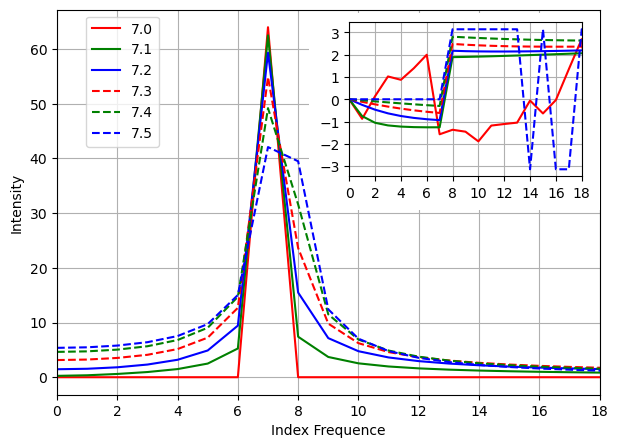
\includegraphics[height=2.5in]{FFT_Unfaithful.png} 
\captionof{figure}{An unfaithful Discrete Fourier transformation is demonstrated by the spectra of a few sine signals having amplitude of 1 and slightly different frequencies as shown in legends.
The x-axis shows the scale for the index frequency.  
The y-axis shows the scale for the intensity, while the y-axis of the embedded picture shows the scale for the phase.
This figure is a practical reproduction of a previous theoretical figure \cite{Prev_Precision_Arithmetic}.
}
\label{fig: FFT_Unfaithful}
\end{figure}

Due to its width, a frequency component in an unfaithful transformation may interact with other frequency components of the Discrete Fourier spectrum, thus sabotaging the whole idea of using the Fourier Transformation to decompose a signal into independent frequency components.  
Because the reverse discrete Fourier transformation mathematically restores the original $\{h[k]\}$ for any $\{H[n]\}$, it exaggerates and narrows all unfaithful signal components correspondingly.  
This means that the common method of signal processing in the Fourier space \cite{Numerical_Recipes}\cite{Stochastic_Arithmetic}\cite{Floating-point_Digital_Filters} may generate artifacts due to its uniform treatment of faithful and unfaithful signal components, which probably coexist in reality.  
Unlike aliasing \cite{Electronics}\cite{Numerical_Recipes}\cite{Floating-point_Digital_Filters}, unfaithful representation of the discrete Fourier transformation has an equal presence in the whole frequency range so that it cannot be avoided by sampling the original signal differently.

An unfaithful representation arises from the implied assumption of the discrete Fourier transformation.  
The continuous Fourier transformation has an infinitive signal range so that:
\begin{equation}
\label{eqn: Fourier continuous shift}
h(t) \Leftrightarrow H(s): \eqspace h(t - \tau) \Leftrightarrow H(s) e^{i 2\pi s \tau};
\end{equation}
As an analog, the discrete Fourier transformation $G[n]$ of the signal $h[k], k = 1 \dots N$ can be calculated mathematically from the discrete Fourier transformation $H[n]$ of $h[k], k = 0\dots N-1$:
\begin{equation}
\label{eqn: Fourier discrete shift}
G[n] = (H[n] + h[N] - h[0]) e^{i 2\pi n/N};
\end{equation}
Applying Formula \eqref{eqn: Fourier continuous shift} to Formula \eqref{eqn: Fourier discrete shift} results in Formula \eqref{eqn: Fourier discrete assumption}.
\begin{equation}
\label{eqn: Fourier discrete assumption}
h[N] = h[0];
\end{equation}
Thus, the discrete Fourier transformation has an implied assumption that the signal $h[k]$ repeats itself outside the region of $[0, N-1]$ \cite{Numerical_DFT}.  
For an unfaithful frequency, $h[N-1]$ and $h[N]$ are discontinuous in regard to signal periodicity, resulting in larger peak width, lower peak height, and the wrong phase.  

The unfaithfulness of the discrete Fourier transformation to the Fourier transformation is a very serious example of modeling errors, but this problem has not be addressed seriously enough previously.
Because the discrete Fourier transformation has widest applications in science and engineering, this problem need some serious attention.


\subsection{FFT (Fast Fourier Transformation)}

\iffalse

Forward:
\begin{align*}
L = 1:\;& o=0: & [0, 1]; \\
 & o = 1: & F = [0 + 1, 0 - 1]; \\
L = 2:\;& o=0: & [0, 2, 1, 3]; \\
 & o = 1: & [0 + 2, 0 - 2, 1 + 3, 1 - 3]; \\
 & o = 2: & [0 + 1 + 2 + 3, 0 + i 1 - 2 - i 3 , 0 - 1 + 2 - 3, 0 - i 1 - 2 + i 3; \\
 & [0, 1, 0, -1]:& [0, i 2, 0, - i 2]; \\
 & [1, 0, -1, 0]:& [0, 2, 0, 2];
\end{align*}

Reverse:
\begin{align*}
L = 1:\;& o=0: & [0, 1]; \\
 & o = 1: & F = [0 + 1, 0 - 1]; \\
L = 2:\;& o=0: & [0, 2, 1, 3]; \\
 & o = 1: & [0 + 2, 0 - 2, 1 + 3, 1 - 3]; \\
 & o = 2: & [0 + 1 + 2 + 3, 0 - i 1 - 2 + i 3 , 0 - 1 + 2 - 3, 0 + i 1 - 2 - i 3; \\
 & [0, i 2, 0, - i 2]:& [0, 4, 0, -4]; \\
 & [0, 2, 0, 2]:& [4, 0, -4, 0];
\end{align*}

\fi

When $N = 2^{L}$, in which $L$ is a positive integer, the generalized Danielson-Lanczos lemma \cite{Numerical_Recipes} can be applied to the discrete Fourier transformation as FFT \cite{Numerical_Recipes}. 
\begin{itemize}

\item For each output, each input is only used once, so there is no dependency problem when using Formula \eqref{eqn: addition and subtraction} and \eqref{eqn: multiplication} as arithmetic operations.
This simplicity avoids introducing numerical errors from Formula \eqref{eqn: Taylor 1d variance}, because $f^{(j)}_x$ may contain numerical errors, while $(\delta x)^{2n}$ may contain rounding errors.

\item When $L$ is large, the large amount of input and output data enables high quality statistical analysis.

\item The amount of calculation is $L$, because for each output, increasing $L$ by 1 results in one additional step of sum of multiplication.

\item Each step in the forward transformation thus increase the variance by $2$-fold, so that the result uncertainty means increase with the FFT order $L$ as $\sqrt{2}^L$.
Because the reverse transformation divides the result by $2^L$, the result uncertainty means decrease with the FFT order $L$ as $\sqrt{1/2}^L$.
The result uncertainty means for the roundtrip transformations is thus: $\sqrt{2}^L \times \sqrt{1/2}^L = 1$.

\item The forward and reverse transformations are identical except a sign, so they are essentially the same algorithm, and their difference is purely due to input data.  

\end{itemize}

A major question for variance arithmetic is that whether the uncertainties can track the the corresponding value errors effectively or not.
FFT transformations provide an ideal test for this statistical property: To test if the error deviations can be close to 1 with the increasing FFT order:
\begin{itemize}
\item The forward transformation cancels real imprecise data of a Sin/Cos signal into a spectrum of mostly $0$ values, so that both its value errors and its result uncertainties are expected to grow faster. 

\item In contrast, the reverse transformation spread the spectrum of precise $0$ values except at two peaks to data of a Sin/Cos signal, so that both its value errors and its result uncertainties are expected to grow slower. 
\end{itemize}




\subsection{Testing Signals}

Only Formula \eqref{eqn: Fourier forward} and \eqref{eqn: Fourier reverse} with integer $n$ and $k$ will be used.

The following signals are used for testing:
\begin{itemize}
\item \emph{Sin}: $h[k] = \sin(2\pi k f/N), f = 1, 2, ... N/2 -1$.

\item \emph{Cos}: $h[k] = \cos(2\pi k f/N), f = 1, 2, ... N/2 -1$.

\item \emph{Linear}: $h[k] = k$, whose discrete Fourier transformation is Formula \eqref{eqn: Fourier spec for linear}.
\begin{align}
& y \equiv i 2\pi \frac{n}{N}: \eqspace G(y) = \sum_{k=0}^{N-1}  e^{y k} = \frac{e^{N y} - 1}{e^y - 1}
 = \begin{cases} y = 0: \eqspace N \\ y \neq 0: \eqspace 0 \end{cases}; \nonumber \\
\label{eqn: Fourier spec for linear}
H[n] &= \frac{d G}{d y} = \begin{cases} n = 0: \eqspace \frac{N (N-1)}{2} \\ n \neq 0: \eqspace - \frac{N}{2}(1 + i /\tan(n \frac{\pi}{N})) \end{cases};
\end{align}

\end{itemize}

Empirically, using the indexed sine functions:
\begin{itemize}
\item The results from Sin and Cos signals are statistically indistinguishable from each other.

\item The results from Sin signals at different frequencies are statistically indistinguishable from each other.
\end{itemize}
So the results for Sin and Cos signals at all frequencies are pooled together for the statistical analysis, as the \emph{Sin/Cos} signals.


\subsection{Library Errors}

\begin{figure}[p]
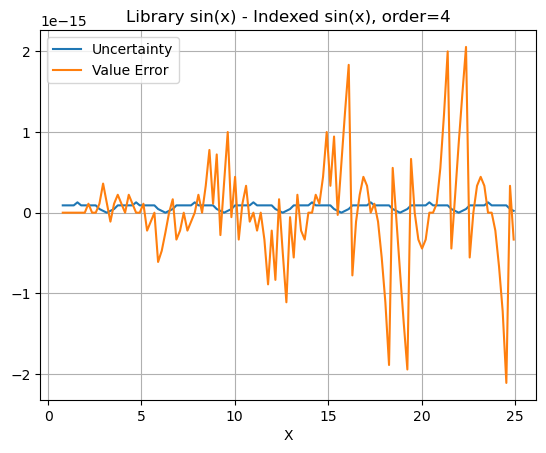
\includegraphics[height=2.75in]{Sin_Diff.png} 
\captionof{figure}{
The difference between the library $\sin(x)$ and the indexed $\sin(x)$, for all integer input to the indexed sine functions used in the FFT transformations of FFT order $4$.
The uncertainty of the $\sin(x)$ values are also displayed, to mark the periodicity of $\pi$.
}
\label{fig: Sin_Diff}
\end{figure}

\begin{figure}[p]
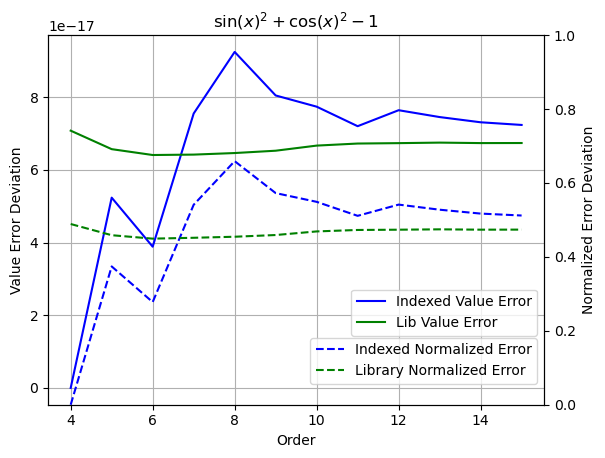
\includegraphics[height=2.75in]{Sin_Error.png} 
\captionof{figure}{
The difference between the library $\sin(x)$ and $\sin(j 2\pi 2^4/2^6)$.   
$\sin(j 2\pi 2^4/2^6)$ has precise values $[0,1,0,-1,\dots]$, so that the corresponding least significant values are $[\;0,2.2 \; 10^{-16},\;0,2.2 \; 10^{-16},\dots]$.
}
\label{fig: Sin_Error}
\end{figure}

\begin{figure}[p]
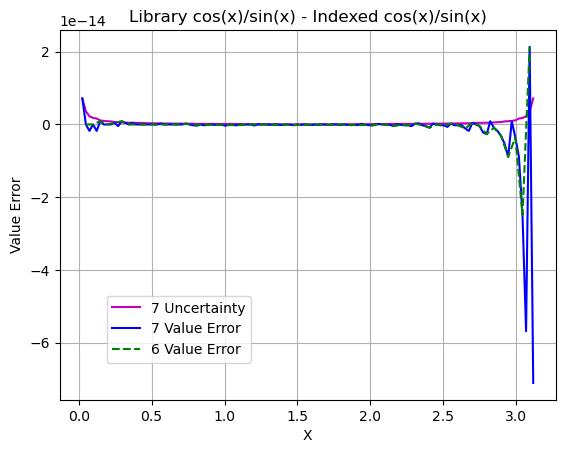
\includegraphics[height=2.75in]{Cot_Diff.png} 
\captionof{figure}{
The difference between the library $\cos(x)/\sin(x)$ and the indexed $\cos(x)/\sin(x)$, for $x \in (0, \pi)$.
}
\label{fig: Cot_Diff}
\end{figure}

\begin{figure}
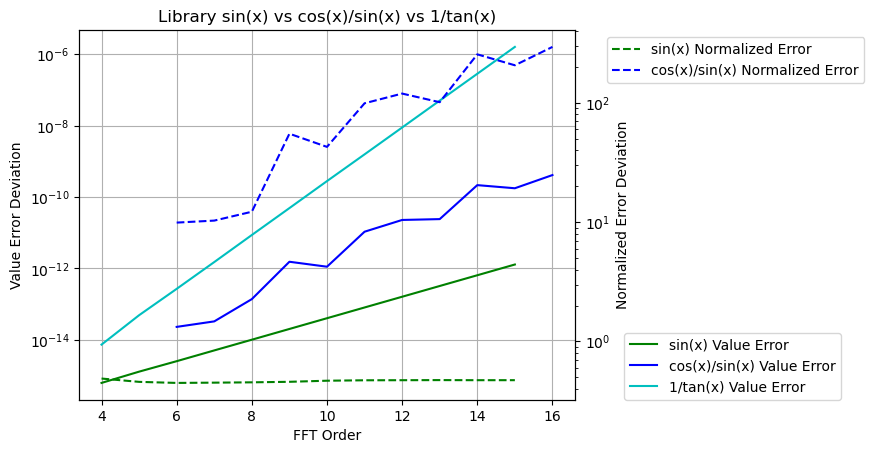
\includegraphics[height=2.75in]{Sin_Cot_Diff.png} 
\captionof{figure}{
Comparing the indexed sine functions and the library sine functions for different FFT orders.
The dashed line is the error deviations of $\sin(x)^2 + \cos(x)^2 - 1$ for the indexed sine functions.
Its y-axis is on the left.
The two solid lines are the maximal absolute value errors of the library $\sin(x)$ and $\cos(x)/\sin(x)$ when compared with the indexed $\sin(x)$ and $\cos(x)/\sin(x)$.  
Their y-axis is on the right.
}
\label{fig: Sin_Cot_Diff}
\end{figure}


Formula \eqref{eqn: Fourier forward} and \eqref{eqn: Fourier reverse} limit the use of $\sin(x)$ and $\cos(x)$ to $x = 2\pi j/N$.
To minimize the numerical errors of $\sin(x)$ and $\cos(x)$, \emph{indexed sine functions} can be used instead of the library sine functions:
\begin{enumerate}
\item Instead of a floating-point value $x$ for $\sin(x)$ and $\cos(x)$, the integer $j$ is used to specify the input to $\sin(x)$ and $\cos(x)$, as $\sin(2\pi j/N)$ and $\cos(2\pi j/N)$, to avoid the floating-point rounding error of $x$.

\item The values of the indexed sine functions is extended from $j = 0,1,\dots N/8$ to the whole integer region using the periodicity of $\sin(2\pi j/N)$ and $\cos(2\pi j/N)$.

\end{enumerate}

Figure \ref{fig: Sin_Diff} shows that the value errors between the library $\sin(x)$ and the indexed $\sin(x)$ increases with increasing $x$ for FFT order $4$.
To confirm Figure \ref{fig: Sin_Diff}, Figure \ref{fig: Sin_Error} shows that the value errors of the library $\sin(x)$ for $\sin(j 2\pi 2^4/2^6)$ increases with increasing $j$. 
The $x$ range in Figure \ref{fig: Sin_Diff} covers all the input used in the FFT transformations of FFT order $4$.
The errors are also periodic in $x$ by $\pi$, which may be amplified in the FFT calculations.

Figure \ref{fig: Cot_Diff} shows the value errors between the library $1/\tan(x)$ and the indexed $1/\tan(x)$ for $x \in (0, \pi)$.
It covers all the integer inputs to the indexed cotan functions used for the Linear signal of FFT order $6$ and $7$.
The value errors near $x = \pi$ increase with the FFT order.

Using the maximal absolute value errors, Figure \ref{fig: Sin_Cot_Diff} compares the value error strengths of the library $\sin(x)$ and $1/\tan(x)$ for increasing FFT orders.
Figure \ref{fig: Sin_Cot_Diff} also shows that when checked by $\sin(x)^2 + \cos(x)^2 - 1$, the obtained indexed sine functions have proper coverage.
In contrast, Figure \ref{fig: Sin_Diff}, \ref{fig: Sin_Error}, and \ref{fig: Cot_Diff} all show that the library $\sin(x)$ and $1/\tan(x)$ do not have proper coverage.

It is clear that the indexed sine functions are much better than the library sine functions.
Sadly, in reality, the library sine functions are used ubiquitously, so that both needs to be evaluated.

\subsection{Using the Indexed Sine Functions for Sin/Cos Signals}

\begin{figure}[p]
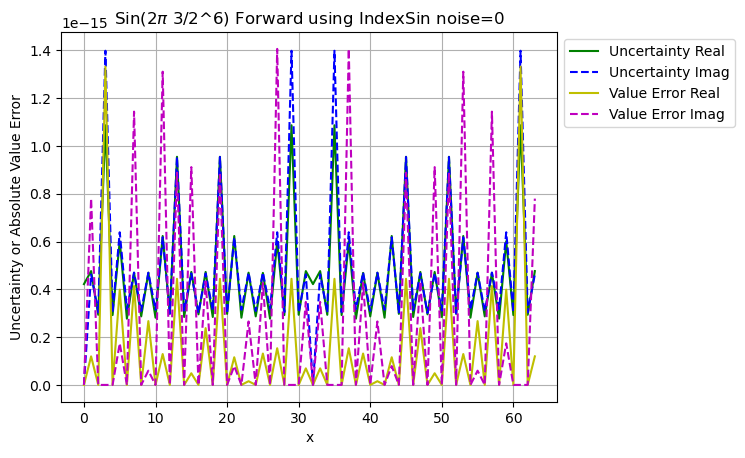
\includegraphics[height=2.75in]{FFT_Sin_Clean_6_3_Spec_Indexed.png} 
\captionof{figure}{
The FFT spectrum of $\sin(j 3/2^6 \pi)$ using the indexed sine functions after the forward transformation calculated by variance arithmetic, with the uncertainty and the value errors shown in the legend.
The x-axis shows the scale for index frequency.
The y-axis shows the scale for uncertainty and absolute value errors.
}
\label{fig: FFT_Sin_Clean_6_3_Spec_Indexed}
\end{figure}

\begin{figure}[p]
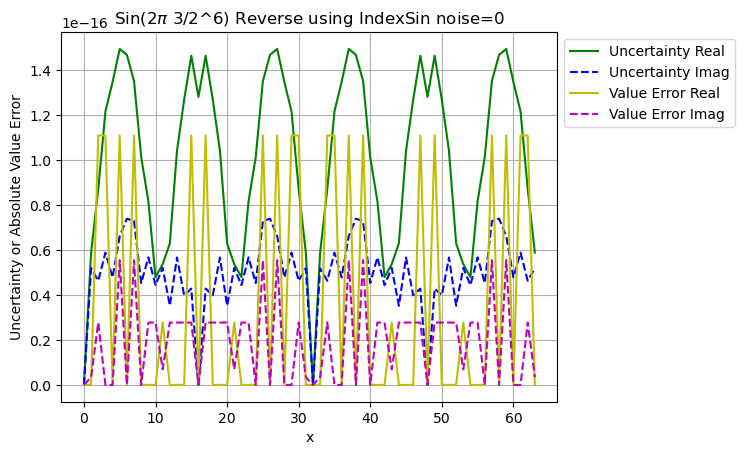
\includegraphics[height=2.75in]{FFT_Sin_Clean_6_3_Wave_Indexed.png} 
\captionof{figure}{
The FFT waveform of $\sin(j 3/2^6 \pi)$ using the indexed sine functions after the reverse transformation calculated by variance arithmetic, with the uncertainty and the value errors shown in the legend.
The x-axis shows the scale for index time.
The y-axis shows the scale for uncertainty and absolute value errors.
}
\label{fig: FFT_Sin_Clean_6_3_Wave_Indexed}
\end{figure}

\begin{figure}[p]
\centering
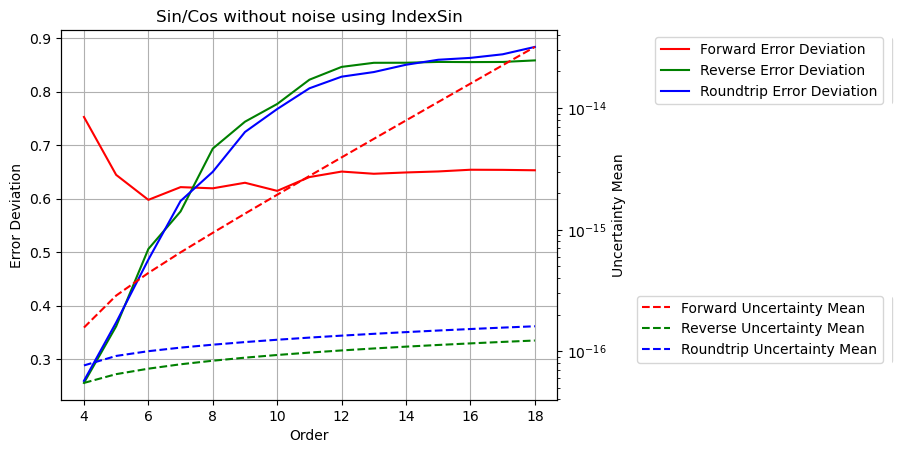
\includegraphics[height=2.5in]{FFT_SinCos_Clean_vs_Order_Indexed.png} 
\captionof{figure}{
The result error deviations and uncertainty means of Sin/Cos signals vs. FFT order using the indexed sine functions for forward, reverse and roundtrip FFT transformations, as shown in the legend.
The error deviations are scaled to the linear y-axis on the left, while the uncertainty means are scaled to the logarithmic log y-axis on the right.
}
\label{fig: FFT_SinCos_Clean_vs_Order_Indexed}
\end{figure}


\begin{figure}[p]
\centering
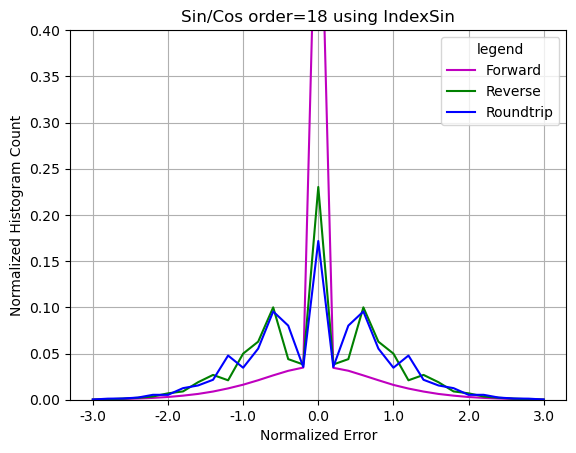
\includegraphics[height=2.5in]{FFT_SinCos_Clean_Histo_Indexed.png} 
\captionof{figure}{
The histograms of the normalized errors of Sin/Cos signals without input noises using the indexed sine functions for forward, reverse and roundtrip FFT transformations, as shown in the legend.
The FFT order is $18$.
}
\label{fig: FFT_SinCos_Clean_Histo_Indexed}
\end{figure}

Using the indexed sine functions, for the waveform of $\sin(2\pi k 3/2^6)$ in which $k$ is the index time:
\begin{itemize}
\item Figure \ref{fig: FFT_Sin_Clean_6_3_Spec_Indexed} shows that for the forward transformation,  the result value errors are comparable to the result uncertainties, with an error deviation of $0.37$ for the real part, and $0.93$ for the imaginary part.

\item Figure \ref{fig: FFT_Sin_Clean_6_3_Wave_Indexed} shows that for the reverse transformation, the result value errors are comparable to the result uncertainties, with an error deviation of $0.54$ for the real part, and $0.52$ for the imaginary part.

\end{itemize}

Figure \ref{fig: FFT_SinCos_Clean_vs_Order_Indexed} shows both the result uncertainty means and the error deviations vs. FFT order of FFT transformations of Sin/Cos signals using the indexed sine functions.
Figure \ref{fig: FFT_SinCos_Clean_Histo_Indexed} shows the corresponding histograms at FFT order $17$.
\begin{itemize}
\item As expected, the uncertainties grow much faster with the increasing FFT order for the forward transformation than those for the reverse transformation.
Both are faster enough to achieve proper coverage. 

\item The faster growth of the uncertainties of the forward transformation in Figure \ref{fig: FFT_SinCos_Clean_vs_Order_Indexed} results in almost Gaussian distribution of the normalized errors for FFT order $18$ in Figure \ref{fig: FFT_SinCos_Clean_Histo_Indexed}.
Thus, the forward transformation is expected to reach ideal coverage quicker with any added noise, and it is less sensitive to numerical calculation errors.

\item The slower growth of the uncertainties of the reverse transformation in Figure \ref{fig: FFT_SinCos_Clean_vs_Order_Indexed} results in structured distribution on top of a Gaussian distribution of the normalized errors for FFT order $18$ in Figure \ref{fig: FFT_SinCos_Clean_Histo_Indexed}.
Thus, the reverse transformation is expected to reach ideal coverage slower with added input noises, and it is more sensitive to numerical calculation errors.

\item With the increasing FFT order, all histograms become more Gaussian like, and the error deviations for the real and the imaginary parts become more equal in value.
The error deviations for the forward transformation are relatively stable.
The error deviations for the reverse transformation increase with the increasing FFT orders until become stable when FFT orders is $12$ or more.
When the FFT order is about $12$, statistical stability is reach.
 
\end{itemize}

Thus, proper coverage is achieved using the indexed sine functions for Sin/Cos signals.


\subsection{Using the Library Sine Functions for Sin/Cos Signals}

\begin{figure}[p]
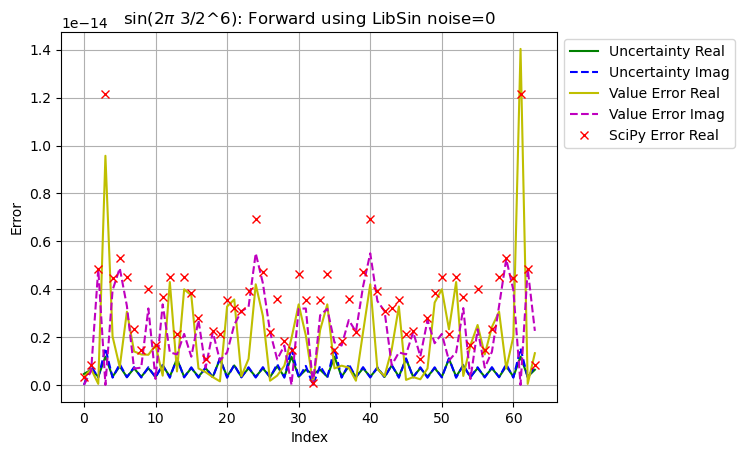
\includegraphics[height=2.5in]{FFT_Sin_Clean_6_3_Spec_Lib.png} 
\captionof{figure}{
The FFT spectrum of $\sin(j 3/2^6 \pi)$ using the library sine functions after the forward transformation calculated by variance arithmetic, with the uncertainties and the value errors shown in the legend.
Also included is the corresponding result errors using \textit{SciPy}.
The x-axis shows the scale for index frequency.
The y-axis shows uncertainties or absolute value errors.
}
\label{fig: FFT_Sin_Clean_6_3_Spec_Lib}
\end{figure}

\begin{figure}[p]
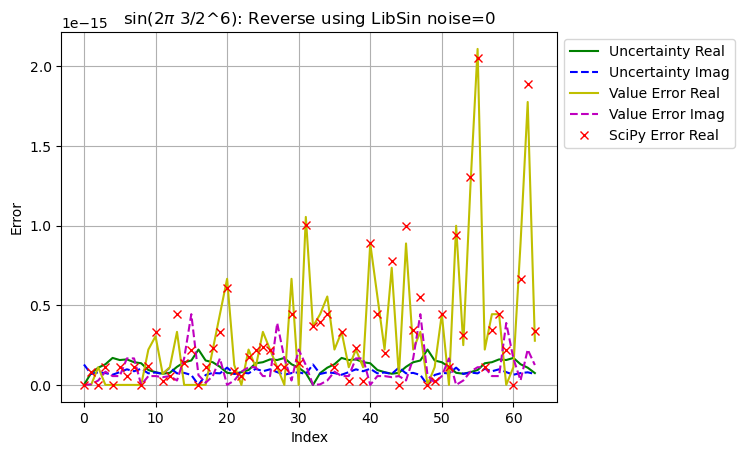
\includegraphics[height=2.5in]{FFT_Sin_Clean_6_3_Wave_Lib.png} 
\captionof{figure}{
The FFT waveform of $\sin(j 3/2^6 \pi)$ using the indexed sine functions after the reverse transformation calculated by variance arithmetic, with the uncertainties and the value errors shown in the legend.
Also included is the corresponding result errors using \textit{SciPy}.
The x-axis shows the scale for index time.
The y-axis shows the uncertainties or absolute value errors.
No input noise is added to the Sin signal.
}
\label{fig: FFT_Sin_Clean_6_3_Wave_Lib}
\end{figure}

\begin{figure}[p]
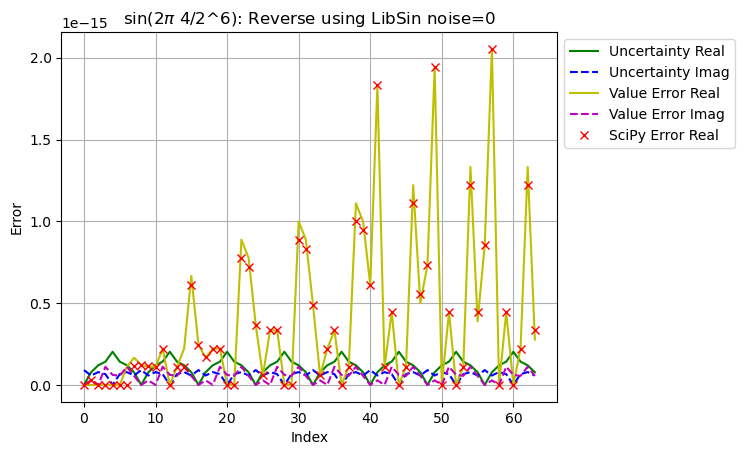
\includegraphics[height=2.5in]{FFT_Sin_Clean_6_4_Wave_Lib.png} 
\captionof{figure}{
The FFT waveform of $\sin(j 4/2^6 \pi)$ using the indexed sine functions after the reverse transformation calculated by variance arithmetic, with the uncertainties and the value errors shown in the legend.
Also included is the corresponding result errors using \textit{SciPy}.
The x-axis shows the scale for index time.
The y-axis shows the uncertainties or absolute value errors.
No input noise is added to the Sin signal.
}
\label{fig: FFT_Sin_Clean_6_4_Wave_Lib}
\end{figure}

\begin{figure}[p]
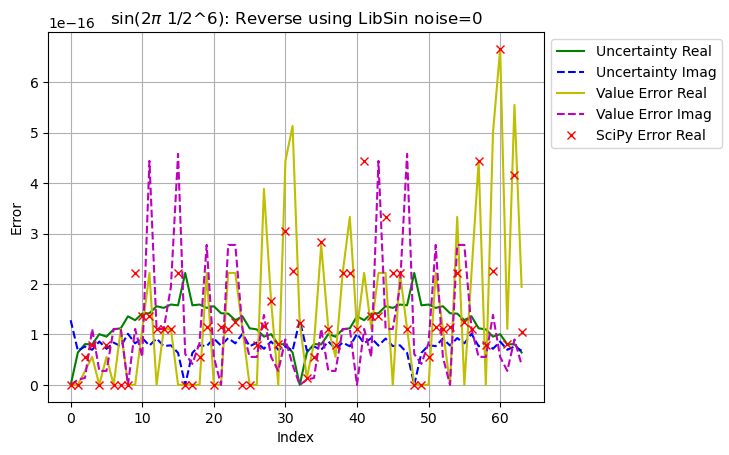
\includegraphics[height=2.5in]{FFT_Sin_Clean_6_1_Wave_Lib.png} 
\captionof{figure}{
The FFT waveform of $\sin(j 1/2^6 \pi)$ using the indexed sine functions after the reverse transformation calculated by variance arithmetic, with the uncertainties and the value errors shown in the legend.
Also included is the corresponding result errors using \textit{SciPy}.
The x-axis shows the scale for index time.
The y-axis shows the uncertainties or absolute value errors.
No input noise is added to the Sin signal.
}
\label{fig: FFT_Sin_Clean_6_1_Wave_Lib}
\end{figure}

\begin{figure}[p]
\centering
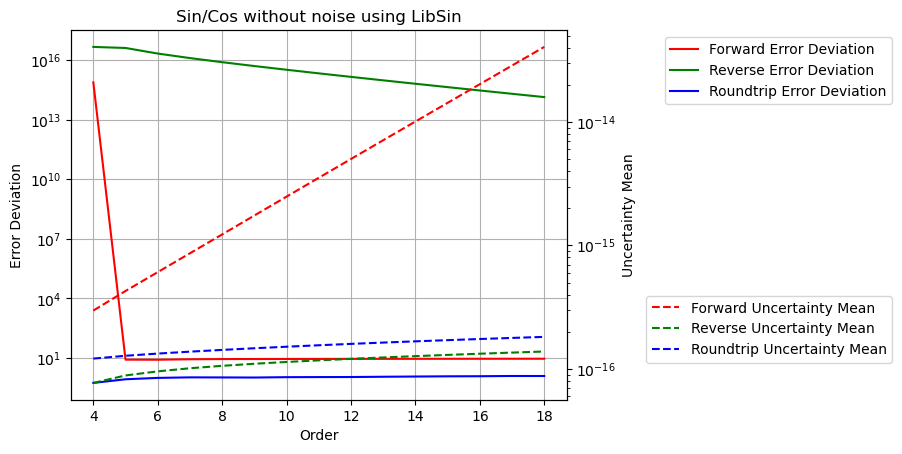
\includegraphics[height=2.5in]{FFT_SinCos_Clean_vs_Order_Lib.png} 
\captionof{figure}{
The result error deviations and uncertainty means of Sin/Cos signals vs. FFT order using the library sine functions for forward, reverse and roundtrip FFT transformations, as shown in the legend.
The error deviations are scaled to the linear y-axis on the left, while the uncertainty means are scaled to the logarithmic log y-axis on the right.
No input noise is added to the Sin signal.
}
\label{fig: FFT_SinCos_Clean_vs_Order_Lib}
\end{figure}

\begin{figure}[p]
\centering
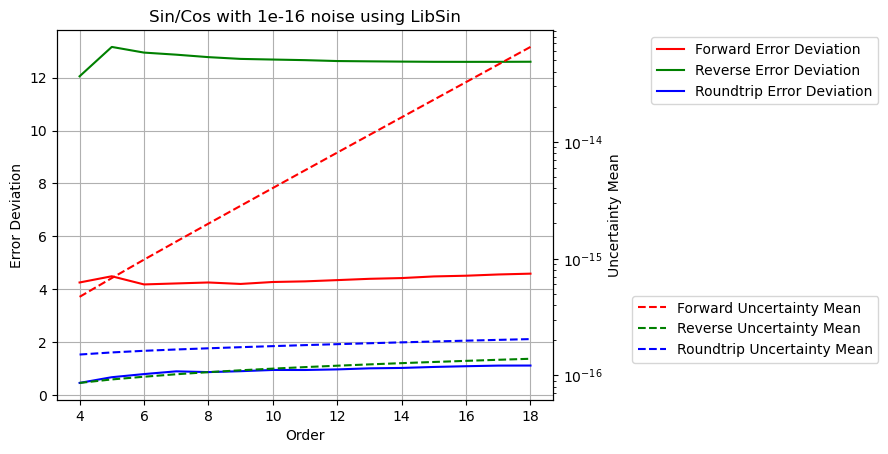
\includegraphics[height=2.5in]{FFT_SinCos_1e-16_vs_Order_Lib.png} 
\captionof{figure}{
The result error deviations and uncertainty means of Sin/Cos signals vs. FFT order using the library sine functions for forward, reverse and roundtrip FFT transformations, as shown in the legend.
The error deviations are scaled to the linear y-axis on the left, while the uncertainty means are scaled to the logarithmic log y-axis on the right.
$10^{-16}$ input noises are added to the Sin/Cos signals.
}
\label{fig: FFT_SinCos_1e-16_vs_Order_Lib}
\end{figure}



Because the least significant values are the only source of input uncertainties for variance arithmetic, the result uncertainties using either sine functions are almost identical.

The library sine functions contributes to the numerical calculation errors which is not specified by the input uncertainties of variance arithmetic.
The question is whether variance arithmetic can track this large amount of numerical errors effectively or not.

Using the library sine functions, for the waveform of $\sin(2\pi k 3/2^6)$ in which $k$ is the index time:
\begin{itemize}
\item Figure \ref{fig: FFT_Sin_Clean_6_3_Spec_Lib} shows that for the forward transformation, the result value errors are noticeably larger than the result uncertainties, with an error deviation of $7.0$ for the real part, and $5.6$ for the imaginary part.
As expected, the error deviations are noticeably larger than their counterparts in Figure \ref{fig: FFT_Sin_Clean_6_3_Spec_Indexed}.

\item Figure \ref{fig: FFT_Sin_Clean_6_3_Wave_Lib} shows that for the reverse transformation, the result value errors are noticeably larger than the result uncertainties, with an error deviation of $5.7$ for the real part, and $	0.83 \; 10^{15}$ for the imaginary part. 
The surprisingly large imaginary error deviation is caused by the small uncertainty at the index time where the value error is at a local maximum.

\item As the result of of the huge error deviation, Figure \ref{fig: FFT_SinCos_Clean_vs_Order_Lib} shows that the result of the reverse transformation no longer has proper coverage for all FFT orders.
When a small noise with deviation of $10^{16}$ is added to the input, the result uncertainty of the reverse transformation at the index time of $8$ is no longer near $0$, so that the result error deviations achieve proper coverage again, as show in Figure \ref{fig: FFT_SinCos_1e-16_vs_Order_Lib}.

\end{itemize}

To validate the FFT implementation in variance arithmetic, the results are compared with the corresponding calculations using the python numerical library \textit{SciPy} in Figure \ref{fig: FFT_Sin_Clean_6_3_Spec_Lib} and \ref{fig: FFT_Sin_Clean_6_3_Wave_Lib}.
The results are quite comparable, except that in \textit{SciPy}, the data waveform is always real rather than complex.
In Figure \ref{fig: FFT_Sin_Clean_6_3_Spec_Lib}, the \textit{SciPy} results have been made identical for the frequency indexes $f$ and $-f$, and the matching to the corresponding results of variance arithmetic is indicative.
In Figure \ref{fig: FFT_Sin_Clean_6_3_Wave_Lib}, the \textit{SciPy} results matches the corresponding results of variance arithmetic well.

In Figure \ref{fig: FFT_Sin_Clean_6_3_Wave_Lib}, the value errors tend to increase with the indexes, which is due to the periodic increase of the numerical errors of $\sin(x)$ with $x$ as shown in Figure \ref{fig: Sin_Diff}.
When the signal frequency increases, the increase of the value errors with the index frequency in the reverse transformation becomes stronger, as shown in Figure \ref{fig: FFT_Sin_Clean_6_1_Wave_Lib}, \ref{fig: FFT_Sin_Clean_6_3_Wave_Lib}, and \ref{fig: FFT_Sin_Clean_6_4_Wave_Lib}.
On the other hand, Figure \ref{fig: FFT_Sin_Clean_6_3_Wave_Indexed} show no such increase, because it contains no library errors as described in Figure \ref{fig: Sin_Diff}.

variance arithmetic reveals the reason why to add small noises to the numerically generated input data, which is already a common practice \cite{Numerical_Recipes}.
How much noises to add to input to achieve proper coverage remains an art.
When the proper tracking of variance arithmetic is not achieved, the result may contain large amount of errors.


\subsection{Linear Signal}

\begin{figure}[p]
\centering
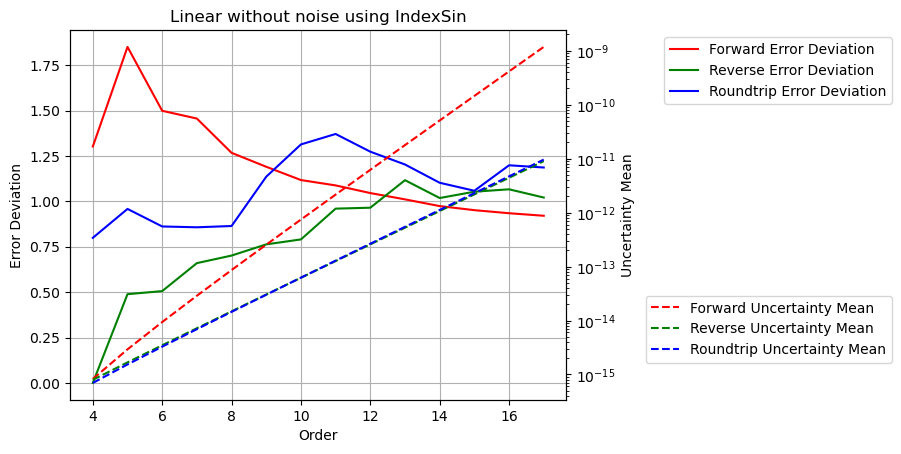
\includegraphics[height=2.5in]{FFT_Linear_Clean_vs_Order_Indexed.png} 
\captionof{figure}{
The result error deviations and uncertainty means of Linear signal vs. FFT order using the library sine functions for forward, reverse and roundtrip FFT transformations, as shown in the legend.
The error deviations are scaled to the linear y-axis on the left, while the uncertainty means are scaled to the logarithmic log y-axis on the right.
No input noise is added to the Linear signal.
}
\label{fig: FFT_SinCos_Linear_vs_Order_Indexed}
\end{figure}

\begin{figure}[p]
\centering
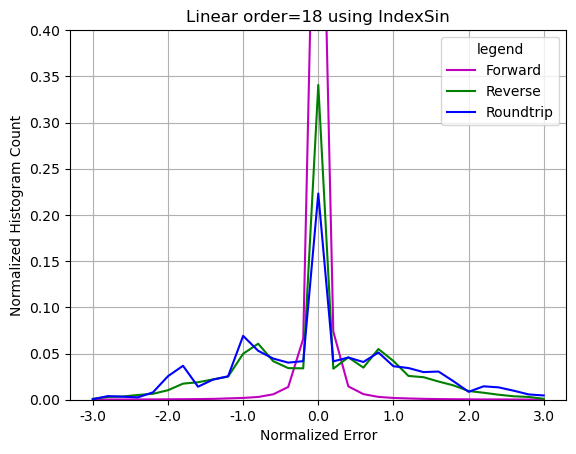
\includegraphics[height=2.5in]{FFT_Linear_Clean_Histo_Indexed.png} 
\captionof{figure}{
The histograms of the normalized errors of Sin/Cos signals without input noises using the indexed sine functions for forward, reverse and roundtrip FFT transformations, as shown in the legend.
No input noise is added to the Linear signal.
}
\label{fig: FFT_Linear_Clean_Histo_Indexed}
\end{figure}

\begin{figure}[p]
\centering
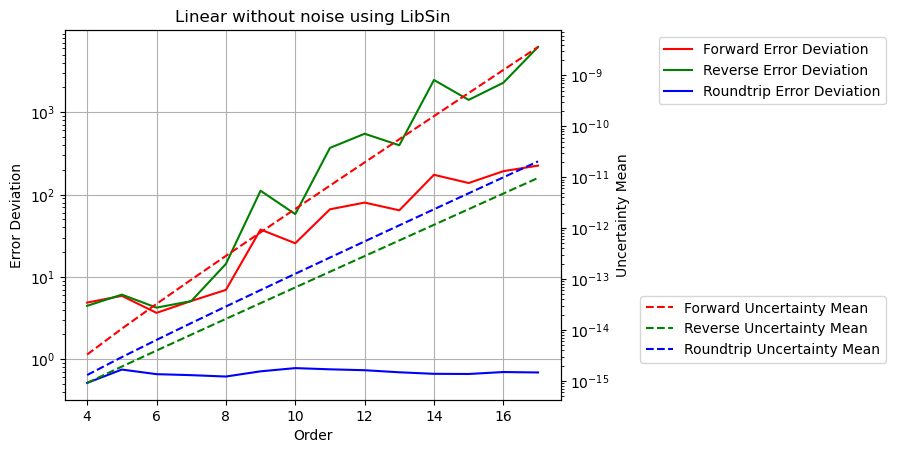
\includegraphics[height=2.5in]{FFT_Linear_Clean_vs_Order_Lib.png} 
\captionof{figure}{
The result error deviations and uncertainty means of Linear signal vs. FFT order using the library sine functions for forward, reverse and roundtrip FFT transformations, as shown in the legend.
The error deviations are scaled to the linear y-axis on the left, while the uncertainty means are scaled to the logarithmic log y-axis on the right.
No input noise is added to the Linear signal.
}
\label{fig: FFT_SinCos_Linear_vs_Order_Lib}
\end{figure}

\begin{figure}[p]
\centering
\includegraphics[height=2.5in]{FFT_Linear_Clean_Histo_Lib.png} 
\captionof{figure}{
The histograms of the normalized errors of Sin/Cos signals without input noises using the indexed sine functions for forward, reverse and roundtrip FFT transformations, as shown in the legend.
No input noise is added to the Linear signal.
}
\label{fig: FFT_Linear_Clean_Histo_Lib}
\end{figure}

In addition to the  numerical errors of $\sin(\pi j /2^L), j = 0, 1, 2 ... 2^{L-1}$, Linear signals introduce the numerical errors of $1/\tan(\pi (j - 1) /2^L), j = 1, 2 ... 2^{L-1}$ to the result.
The question is whether variance arithmetic can track this additional numerical errors or not.

Using the indexed sine functions:
\begin{itemize}
\item Figure \ref{fig: FFT_SinCos_Linear_vs_Order_Indexed} shows that proper coverage can be achieved for all the FFT transformations for all FFT orders.

\item Figure \ref{fig: FFT_Linear_Clean_Histo_Indexed} shows that for each transformation, the histogram of the Linear signal are quite quite similar to the counterpart of the Sin/Cos signals in Figure \ref{fig: FFT_SinCos_Clean_Histo_Indexed}. 

\end{itemize}
 
Using the library sine functions:
\begin{itemize}
\item Figure \ref{fig: FFT_SinCos_Linear_vs_Order_Lib} shows that proper coverage can not be achieved any FFT transformation for all FFT orders, because the value errors outpace the uncertainties with the increasing FFT order.
Because of this, adding noise to the input can not achieve proper coverage.

\item Figure \ref{fig: FFT_Linear_Clean_Histo_Lib} shows that the reverse histogram contains additional peaks in addition to its counterpart in Figure \ref{fig: FFT_SinCos_Linear_vs_Order_Lib}.
The additional peaks extend beyond the range of $[-3, +3]$

\end{itemize}

When too much numerical errors are not specified by the input uncertainties, proper coverage can not be achieved, which is the case when the $\sin(x)$ numerical errors in Figure \ref{fig: Sin_Diff} is combined with the $1/\tan(x)$ numerical errors in Figure \ref{fig: Cot_Diff}.
The only solution seems to create a new sin library using variance arithmetic so that all numerical calculation errors are accounted for.



\subsection{Ideal Coverage}

\begin{figure}[p]
\centering
\includegraphics[height=2.5in]{FFT_SinCos_vs_Noise_Indexed.png} 
\captionof{figure}{
The result error deviations and uncertainty means for Sin/Cos signals of order 16 using indexed sin/cos functions vs. input uncertainties for forward, reverse and roundtrip transformations for FFT order $18$.
The error deviations are scaled to the linear y-axis on the right, while the uncertainty means are scaled to the logarithmic log y-axis on the right.
}
\label{fig: FFT_SinCos_vs_Noise_Indexed}
\end{figure}

\begin{figure}[p]
\centering
\includegraphics[height=2.5in]{FFT_SinCos_vs_Noise_Lib.png} 
\captionof{figure}{
The result error deviations and uncertainty means for Sin/Cos signals of order 16 using library sin/cos functions vs. input uncertainties for forward, reverse and roundtrip transformations for FFT order $18$.
The error deviations are scaled to the linear y-axis on the right, while the uncertainty means are scaled to the logarithmic log y-axis on the right.
}
\label{fig: FFT_SinCos_vs_Noise_Lib}
\end{figure}

\begin{figure}[p]
\centering
\includegraphics[height=2.5in]{FFT_Linear_vs_Noise_Indexed.png} 
\captionof{figure}{
The result error deviations and uncertainty means using Linear signals of order 18 vs. input uncertainties for forward, reverse and roundtrip  transformations for FFT order $18$.
The error deviations are scaled to the linear y-axis on the right, while the uncertainty means are scaled to the logarithmic log y-axis on the right.
}
\label{fig: FFT_Linear_vs_Noise_Indexed}
\end{figure}

\begin{figure}[p]
\centering
\includegraphics[height=2.5in]{FFT_Linear_vs_Noise_Lib.png} 
\captionof{figure}{
The result error deviations and uncertainty means using Linear signals of order 18 vs. input uncertainties for forward, reverse and roundtrip  transformations for FFT order $18$.
The error deviations are scaled to the linear y-axis on the right, while the uncertainty means are scaled to the logarithmic log y-axis on the right.
}
\label{fig: FFT_Linear_vs_Noise_Lib}
\end{figure}

\begin{figure}[p]
\centering
\includegraphics[height=2.5in]{FFT_Linear_1e-3_Histo_Lib.png} 
\captionof{figure}{
The histograms of the normalized errors of Linear signal without input noises using the library sine functions for forward, reverse and roundtrip FFT transformations, as shown in the legend.
$10^{-3}$ input noises are added to the Sin/Cos signals.
}
\label{fig: FFT_Linear_1e-3_Histo_Lib}
\end{figure}

\begin{figure}[p]
\centering
\includegraphics[height=2.5in]{FFT_Linear_1e-3_vs_Order_Lib.png} 
\captionof{figure}{
The result error deviations and uncertainty means using Linear signal with $10^{-3}$ input noises vs. FFT order for forward, reverse and roundtrip FFT transformations.
The error deviations are scaled to the linear y-axis on the left, while the uncertainty means are scaled to the logarithmic log y-axis on the right.
}
\label{fig: FFT_Linear_1e-3_vs_Order_Lib}
\end{figure}

\begin{figure}[p]
\centering
\includegraphics[height=2.5in]{FFT_Linear_Lib_Forward_ErrorDev_vs_Noise_Order.png} 
\captionof{figure}{
The result error deviations for Linear signals using library sine functions vs. input uncertainties and FFT orders for the forward transformations.
The input uncertainties run from $10^{-16}$ to $10^{-1}$, while the FFT Order runs from $6$ to $18$.
}
\label{fig: FFT_Linear_Lib_Forward_ErrorDev_vs_Noise_Order}
\end{figure}

\begin{figure}[p]
\centering
\includegraphics[height=2.5in]{FFT_Linear_Lib_Reverse_ErrorDev_vs_Noise_Order.png} 
\captionof{figure}{
The result error deviations for Linear signals using library sine functions vs. input uncertainties and FFT orders for the reverse transformations.
The input uncertainties run from $10^{-16}$ to $10^{-1}$, while the FFT Order runs from $6$ to $18$.
}
\label{fig: FFT_Linear_Lib_Reverse_ErrorDev_vs_Noise_Order}
\end{figure}

\begin{figure}[p]
\centering
\includegraphics[height=2.5in]{FFT_Linear_Indexed_Forward_ErrorDev_vs_Noise_Order.png} 
\captionof{figure}{
The result error deviations for Linear signals using indexed sine functions vs. input uncertainties and FFT orders for the forward transformations.
The input uncertainties run from $10^{-16}$ to $10^{-1}$, while the FFT Order runs from $6$ to $18$.
}
\label{fig: FFT_Linear_Indexed_Forward_ErrorDev_vs_Noise_Order}
\end{figure}

\begin{figure}[p]
\centering
\includegraphics[height=2.5in]{FFT_Linear_Indexed_Reverse_ErrorDev_vs_Noise_Order.png} 
\captionof{figure}{
The result error deviations for Linear signals using indexed sine functions vs. input uncertainties and FFT orders for the reverse transformations.
The input uncertainties run from $10^{-16}$ to $10^{-1}$, while the FFT Order runs from $6$ to $18$.
}
\label{fig: FFT_Linear_Indexed_Reverse_ErrorDev_vs_Noise_Order}
\end{figure}

Even when proper coverage can not be achieved, adding enough noise to the input can overpower the numerical calculation errors, to achieve ideal coverage.

Figure \ref{fig: FFT_Linear_1e-3_Histo_Lib} shows that with $10^{-3}$ input noise, the result normalized errors for the forward and reverse transformations are both normal distributed, while the result normalized errors for the roundtrip transformation is delta distributed, regardless of the types of input noises.

Figure \ref{fig:  FFT_Linear_1e-3_vs_Order_Lib} shows the result error deviations and uncertainty means vs. different input uncertainties for Linear signal of order $18$ using the library sin/cos functions.  
When the deviation of the input noise is more than $10^{-3}$, the input uncertainties become ideal coverage:
\begin{itemize}
\item As expected, the result uncertainty means for the forward transformations increase with the FFT order $L$ as $\sqrt{2}^L$.

\item As expected, the result uncertainty means for the reverse transformations decrease with the FFT order $L$ as $\sqrt{1/2}^L$.

\item As expected, the result uncertainty means for the roundtrip transformations always equal the corresponding input uncertainties.

\item As expected, the result uncertainty means for both the forward and the reverse transformations are linear to the input uncertainties, respectively, because FFT transformations are linear.
As expected, the result uncertainty means for the roundtrip transformation recover the corresponding input uncertainties perfectly.

\item As expected, the normalized errors for the forward and the reverse transformations are normal distributed, even when the input noise is no longer Gaussian.
The normalized errors for the roundtrip transformations are delta distributed at $0$, meaning the input uncertainties are perfectly recovered.

\item As expected, the result error deviations for the forward and reverse transformations are constant $1$, while the result error deviations for the roundtrip transformation approaches $0$ exponentially with the increasing FFT order.

\end{itemize}

For Linear signals using the library sine functions, the the added noise vs FFT order regions for the ideal coverage are shown as the regions where the error deviations are $1$, by Figure \ref{fig: FFT_Linear_Lib_Forward_ErrorDev_vs_Noise_Order} and \ref{fig: FFT_Linear_Lib_Reverse_ErrorDev_vs_Noise_Order} for the forward and reverse transformations, respectively.
In other regions, proper coverage is not achievable.
Because the uncertainties grow slower in the reverse transformation than in the forward transformation, the reverse transformations have smaller ideal coverage region than that of the forward transformation.
Because the amount of numerical errors increases with the amount of calculations, the input noise range reduces with the increasing FFT order.
It is possible that ideal coverage is not achievable at all, e.g., visually, when the FFT order is larger than $25$ for the reverse transformation.
As one of the most robust numerical algorithm that is very insensitive to input errors, FFT breaks down when the FFT order is more than $25$ due to the numerical errors in the library sine functions, and such deterioration of the calculation result is not easily detectable using the conventional floating-point calculation.

In contrast, for Linear signals using the indexed sine functions, the the added noise vs FFT order regions for the ideal coverage are shown as the regions where the error deviations are $1$, by Figure \ref{fig: FFT_Linear_Indexed_Forward_ErrorDev_vs_Noise_Order} and \ref{fig: FFT_Linear_Indexed_Reverse_ErrorDev_vs_Noise_Order} for the forward and reverse transformations, respectively.
The ideal regions are much larger.
In other regions, proper coverage are achieved.


\subsection{Summary}

Compared to its counterpart continuous Fourier Transformation (FT), the discrete Fourier transformation (DFT) has large modeling error for its implied assumption that any waveform is periodic outside its defined time range.
This modeling error has not been addressed seriously.

The library sine functions using conventional floating-point arithmetic have been shown to contain numerical errors as large as equivalently  $10^{-3}$ of input accuracy for FFT transformations.
The library $\sin(x)$ errors increase periodically with $x$, causing noticeable increase of the result errors with the increasing index frequency in the reverse transformation.
The dependency of the result numerical errors on the amount of calculation and input data means that a small scale test can not properly qualify the result of a large scale calculation.
The effect of numerical errors inside math library has not been addressed seriously.

variance arithmetic should be used, whose values largely reproduce the corresponding results using conventional floating-point arithmetic, whose uncertainties trace all input errors, and whose result error deviations qualify the calculation quality as either ideal, or proper, or suspicious.
If the library functions also have proper coverage, the calculation result will probably have proper coverage as well.











\clearpage
\section{Conclusion and Discussion}
\label{sec: conclusion and discussion}

\subsection{Summary of Variance Arithmetic}

The starting point of variance arithmetic is the uncorrelated uncertainty assumption, which requires input data to have small enough precision as shown in Figure \ref{fig: Independent_Uncertainty_Assumption}.  In addition, it requires that the systematic errors is not the major source of uncertainty.

Once the uncorrelated uncertainty assumption is satisfied, variance arithmetic quantifies uncertainty as the deviation of the value errors.
It can trace the variable dependency in the intermediate steps using standard statistics.
Taylor expansion can be used to obtain the result mean and uncertainty of analytic functions, as Formula \eqref{eqn: Taylor 1d mean}, \eqref{eqn: Taylor 1d variance}, \eqref{eqn: Taylor 2d mean}, \eqref{eqn: Taylor 2d variance}, and etc.
The convergence requirement of variance arithmetic also reject calculations based on input precision, such as inversion of an input which has a high probability of containing zero. 

The ability of variance arithmetic to trace value errors using calculated uncertainties is shown to be very effective:
\begin{itemize}
\item When zero result is expected, the normalized value errors of variance arithmetic is delta distributed.

\item Due to the uncorrelated uncertainty assumption and central limit theorem, the normalized value errors of variance arithmetic are normal distributed.
In the ideal coverage cases when the input uncertainties precisely quantify the corresponding errors, the deviations of the normalized value errors are shown to be $1$.
The ideal coverage defines the ideal applicable range of variance arithmetic.
It is also the necessary condition for any particular application of variance arithmetic to be correct.

\item The floating-point rounding errors are generated in the process of floating-point calculations, so they are not subjected to central limit theorem.
It has been shown that the deviation of the normalized value errors of variance arithmetic are in the range of $[0.25, 4]$, which fails in the range of proper coverage.

\item Another reason of proper coverage is that the input uncertainties do not precisely specify the input errors.

\item When the input uncertainties are two different from the corresponding value errors which they specify, variance arithmetic will not work properly.
Such situation can be detected by the values of the normalized error deviations outside the range of $[0.1, 10]$.
\end{itemize}

variance arithmetic has been shown to be widely applicable, so as for analytic calculations, progressive calculation, regressive generalization, polynomial expansion, statistical sampling, and transformations.


\subsection{The Need for Recalculating Library Math Functions}

The library math functions need to be calculated using variance arithmetic, so that each output value has its corresponding uncertainty.
Otherwise, the effect of the existing value errors in the library function can have unpredictable and large effects.
For example, this paper shows that the periodic numerical errors in the $\sin$ and $\tan$ library functions causes resonant-like large result value errors for the FFT calculations.



\subsection{The Need for New Numerical Approaches}

To properly account for the result uncertainties, analytic expressions are favored over the corresponding numerical approaches, because the convergence of the result uncertainties are generally slower than those of the result values.

The conventional numerical approaches focus primarily on the result values, and they need to be reexamined or even revamped for the result uncertainties.
The input uncertainties cause large uncertainty biases on the corresponding result values in the case of matrix inversion,  and the result precision is generally much worse than the input precision.
One such example is matrix inversion.

Using Taylor expansion approach, it is generally an order-of-magnitude more complicated to calculate the result uncertainties than the result values.
However, modern software programs for analytic calculation can be great help.
Also, the calculation of the result uncertainty is highly paralleliziable, so that modern parallel computing can be great help. 


\subsection{The Need for Different Floating-Point Representation for Variance}

In variance representation $x \pm \delta x$, $\delta x$ is comparable in value with $x$, but $(\delta x)^2$ is calculated and stored.
This limits the effective range for $x \pm \delta x$ to be much smaller than the full range of the standard 64-bit floating-point representation $\pm\; 2^{52} \; 2^{\pm 1024}$, such as when applying Formula \eqref{eqn: Taylor 1d mean} and \eqref{eqn: Taylor 1d variance} to floating-point rounding errors in Section \ref{sec: polynomial}.
Ideally, $(\delta x)^2$ should be calculated and stored in an different 64-bit floating-point representation with the range at least $2^{51} \; 2^{\pm 4096}$ in which  the sign is no longer needed, and the bit count for the significand needs not more than $52$ because $(\delta x)^2$ does not need to be as accurate as $x$.


\subsection{Hardware Implementation}

Because variance arithmetic has neither execution freedoms nor the associated dependency problems, it can be implemented in hardware in CPU or GPU.



\subsection{Acknowledgements}

As an independent researcher, the author of this paper feels indebted to encouragements and valuable discussions with Dr. Zhong Zhong from Brookhaven National Laboratory, Dr. Anthony Begley from \emph{Physics Reviews B}, the organizers of \emph{AMCS 2005}, with Prof. Hamid R. Arabnia from University of Georgia in particular, and the organizers of \emph{NKS Mathematica Forum 2007}, with Dr. Stephen Wolfram in particular. 
The author of this paper is very grateful for the editors and reviewers of \emph{Reliable Computing} for their tremendous help in shaping and accepting the previous version of this paper from unusual source, with managing editor, Prof. Rolph Baker Kearfott in particular.



\bibliographystyle{unsrt}
\bibliography{PrecisionArithmetic}






\end{document}
